

\chapter{Introduction & Executive Summary}
This report you have opened is not monolithic. You can match its sections
to your needs.

The first section introduces our topic. It starts by describing the landscape
where sensors and journalism combine, and continues on to define necessary
terms for understanding this area of research. Reporters are using
sensors in an era when the rapid development of technology is moving data
into the mainstream of journalism. The increasing ubiquity of sensors, their
increasing capability and accessibility are on the supply side, while investigative
reporters, computer aided reporters and journalist/technologists
are on the demand side. We are including drones in the field of sensing,
partially because of the amount of attention they're currently receiving,
and partially because of their potential to extend human sight far beyond
our bodily bounds. While recent commentaries about journalistic sensing
have focused just on sensors that journalists have built themselves (or commissioned),
our definition also includes journalistic uses of data from sensor
systems that are not controlled by the reporters themselves. We have
excluded opinion polling, information gathered by humans' five senses, and
data produced by monitoring computer processes like bit-torrent networks.
That said, our description should not be used to separate sensor-based journalism
from other reporting processes. The intellectual tools we discuss
may be useful for many data-intensive projects, and sensor reporting needs
to be integrated with traditional forms.

Then, scholar Charles Berret has written a chapter on sensor history, charting
humanity's efforts to extend the reach of our five natural senses. It starts
with the scales unearthed by archeologists, the Neolithic markers like Stonehenge,
and the agricultural tools from the Nile region. Berret notes that,
in the 1500's, the astronomer Tycho Brahe built a data network using the
post, which compiled sensor readings to draw the most accurate and comprehensive
star maps of his time. Cameras and sound sensors came in the
nineteenth century, a moment 'when mechanical sensors were first treated
with greater credibility than the human observer.' The history outlined here
only goes as far as the first half of the twentieth century, but within our time
period it covers early medical sensors in the form of René Laennec's stethoscope
and Willem Einthoven's electrocardiogram, and meteorologists' use
of doppler radar.

The introduction finishes by outlining the characteristics of sensors that
make them useful—or not—and helping readers identify what elements of
the world can be sensed.

The second section, containing case studies, examines seven projects that
used sensors for journalism. Each study includes the story of what happened
and then offers analysis in which we identify its distinctive or noteworthy
elements, as well as the lessons journalists may take from the projects.
The case studies start to show distinct types of sensor uses that suit different
journalistic goals. The first type is when investigative reporters (environmental
reporters in these two examples) design a sensing process to collect
data with the intent of testing a hypothesis. They used relatively mature professional
equipment and consulted with experts. They had justifiable confidence
in their data, even though their processes were quite different from
how scientists work when intending to publish in a peer-reviewed journal,
or when doing work on behalf of regulators.

Another type of sensor use by journalists is accessing data from municipal
sensor systems. The Sun Sentinel won a Pulitzer Prize by using tollgate data
to investigate widespread speeding by off duty Florida police. The Washington
Post published an extensive explanatory feature based on data from a
network of microphones installed by the city law enforcement.

A separate type of journalistic sensing involves DIY hardware development.
At the moment, these projects value participation and informal
science education. At the moment the equipment they use is unlikely to
produce data that can be heavily relied upon in legal or health settings.
However, the makers in this part of the field see great long-term potential,
inspired by open-source software, a phenomenon that has returned great
value to newsrooms.

In case studies, we have also added analysis of the U.S. drone journalism
industry, as it stands right now. At the high end, a small number of organizations
are using footage shot by specialist pilots of professional cinematography
drones. In the middle, enterprising news industry employees are
experimenting with pro-am equipment costing hundreds, not thousands of
dollars. Mainstream media organizations are also sourcing drone footage
shot by hobbyists. All of this activity is proceeding despite a rapidly changing,
highly contested regulatory environment.

For the next section, about laws and ethics for reporting with sensors, we
recruited 12 experts to write a chapter each. They applied their considerable
knowledge and ability from professions in law, technology, ethics, academic
research, and the sciences. In the individual essays, each helps identify and
navigate the key issues that arise when their field intersects with sensors
and journalism.

The authors who address the privacy and surveillance issues write that
these are early days for the field. The courts have thus far dealt with consent
to record, defamation and false light in the context of cameras and
microphones. The potential for journalists to break those laws using different
types of sensors certainly exists, and if legal claims are made courts will likely consider the ethical standards that emerge in these next few years of
sensor reporting. The field is emerging even as relationship between newsrooms
and their audiences transforms. Our authors suggest that journalists
should involve their communities as they negotiate the tricky questions of
who owns and controls personal data from sensors.

Newsroom managers who have staff making or acquiring hardware should
also acquaint themselves with the basics of open-source licensing. Often,
journalists who design their own sensing systems will lean towards sharing
their work under open-source principles, but this may involve legal liability
if hardware goes wrong and causes physical damage. The risks are avoidable,
however, as the article by Diana Cooper makes clear.

Still in the realm of legal issues for hardware makers, this current phase of
rapid, widespread DIY development is moving a lot faster than The Federal
Communications Commission. The FCC requires that any electronic device
that might emit radio interference be tested and approved before marketing.
However, that regime did not consider many conceivable journalistic
uses of custom sensors produced in small batches.

If and when sensing, in particular drone use, becomes a widespread journalistic
practice, human error is likely. Serious mistakes will attract negligence
claims, following in a tradition codified by The Digest of Justinian in
the mid-sixth century. It contained a section on 'Those Who Pour or Throw
Things Out of Buildings'. The laws extended to falling things, as well. Despite
this history, the novelty of drone journalism will make insurance tricky and
expensive until the industry has more data on which to model risk profiles.

The last group within the legal and ethical section concerns truth and accuracy.
Sensors may seduce journalists into thinking their output is objective
and free from the errors inherent in human testimony. That is a risky belief.
We have drawn on the expertise of the EPA to show how reporters might
design a sensor-based data collection process to improve their accuracy.
For journalists, the concept of \'ground-truthing\'—supplementing sensor information with human input—will be valuable. It should help introduce
nuance, guard against mistakes and treat fairly the people at the heart of
our stories.

For the final section, we have distilled this report into a set of recommendations,
including groups of strategic moves, good work practices, and efforts
the industry may collectively consider.

\subsection{Strategic Recommendations}
\begin{itemize}
\item Identify and cultivate sensor sources for the beats you've prioritized.
\item Put a watching brief on open source sensing systems.
\item News nerds should do hardware too.
Work Practice Recommendations
\item Before sensing, articulate your hypothesis.
\item Work with experts on complex stories.
\item Understand the entire pipeline for your story's sensor data.
\item Combine sensing with traditional reporting.
Recommendations for the industry, collectively
\item Journalists have an opportunity and a responsibility to report on
sensor systems.
\item Advocate for access to data from publicly funded sensor systems.
However, even though we have documented significant amounts of journalistic
sensing here, we hope that this report will need updates as newsrooms
keep combining their reporters' ideas with new sensing opportunities.
\end{itemize}

\part{The First Section: A Framework}


\chapter{The Landscape for Sensors and Journalism}
Throughout 2013 and 2014, whenever the Tow Center gathered people
together to work on the topic of sensor journalism, we needed to set the
scene. When it comes to labels, ``sensor journalism'' isn't even as understood
as ``data journalism.'' So, although the last thing journalism needs is a new
term to define a fragment of its practice, we must draw some boundaries
and describe the landscape to bring readers of this report into a common
language. Nonetheless, we reserve the right to retreat or advance from this
ground, or even open the borders, as seems necessary in the rapidly evolving
world of journalism circa 2014.

By erecting a frame of reference for journalistic sensing we hope to help
readers efficiently understand which intellectual tools they can apply to
their own sensing and sensor-based work by others. However, by describing
this field discretely we do not mean to advocate that it be practiced discretely
from other types of reporting; quite the opposite. Indeed, the legal
and ethical sections and most of the case studies that follow demonstrate
the value in combining sensor-based reporting with other journalistic tools,
including personal interviews and shoe-leather reporting, so that the data
can be incorporated with context, narrative and emotion.

\subection{King Data and the Wide Angle for Journalism}
First, we offer some observations about why it might be worth focusing on
sensors in combination with journalism. This is the context for this report;
a suggestion of why there is value in this particular vein of research.
Sensors are a way of collecting information about the world. Journalists
trade in acquiring information, analyzing it, organizing it, and distributing
it. That alone suggests a natural fit.

However, beyond that, journalists are currently paying special attention to
data that can be easily parsed by a computer. Many readers of this report
will be familiar with the impact of data-specialist teams put together by the
top tier of American and international news companies, whether in longestablished
newsrooms like The New York Times, the LA Times, the Guardian,
and the Washington Post, or ambitious newcomers like FiveThirtyEight,
Buzzfeed, and Vox.^{\href{#endnotes-landscape}{1}} Journalism schools have recruited professors who teach
data analytics, principles, and presentations. Hundreds of Master of Science
students entering Columbia University's Graduate School of Journalism
in 2013 took at least three seminars about data practices. Many go on to
learn Python and R programming languages in greater depth. The primary
U.S. conference for data journalism, NICAR, went from a conference of a
few hundred people in 2010 to one with a thousand attendees
in 2014.

The rise of data journalism has coincided with an age in which technology
is becoming cheaper, more capable, and more widespread. Many observers
would suggest a causal relationship: When computers permeated more
homes and schools, more children learned programming skills. More systems and data about the world have been digitized. There are more stories to be found in databases and more journalists working in the profession
with the interest and skills to find them.

\subsection{Sensors Everywhere}
The hardware components of technology, including sensors, are also cheaper
and more ubiquitous. While the following examples of sensors don't encompass
the breadth of technology observed in this report, they can be a useful
illustration. Cellphones include cameras, accelerometers, and GPS sensors,
microphones and radio frequency receivers. Those components now cost
a few dollars at wholesale. Young children (or at least their parents) can
spend \$36 to buy a pair of sneakers that sense movement and trigger small
lights in the soles. Sensors are baked into civic processes like traffic control,
and industrial processes like stock control. A private company called Planet
Labs has put 28 toaster-sized satellites into orbit, designed to operate as a
flock of cameras pointed toward the earth. It's aiming to have an array of
100 craft in space by March of 2015. We are living in a sensed world.

Aside from the sensors incorporated into finished products for consumers,
governments, and private enterprise, sensors comprise a key component
class used by the ``maker movement.'' That ecosystem encompasses electronics
prototyping platforms such as Arduino and Raspberry Pie, DIY electronics
retailers Sparkfun and Adafruit, and, if interpreted widely, also includes
KickStarter's crowd-sourced product development and the consumer-side
of 3D printing. Taken together with the spread in programming skills, it is
fair to say that DIY hardware development is flourishing. In early 2013 the
makers of the popular electronic prototyping platform, Arduino, said there
were 700,000 boards in operation. They estimate that the number doubles
if one includes the clones (which are legal, given their open-source license).

So for journalism, there is a special symmetry of demand and supply.
Behind the computer-aided reporters and data savvy journalists have come
a generation of programmer-journalists. They all compete for fresh data to
include in their stories. Another artifact of the digital-first era is the development
of news apps and interactive news graphics, in which users' ability
to explore data requires that information be available in granular form, not
just as a summary paragraph or a static graphic (although those are also
both perfectly justifiable outcomes of a data-reporting process). As the case
studies in this report explore, sensors can produce the data demanded by
computer-aided journalistic processes.

However, beyond simply satisfying the existing demand for data, particular
characteristics of modern sensors and their accompanying technologies
produce opportunities for new reporting processes. The low cost of some
sensor types enables experimentation and new modes of use. In the case
studies that follow, we see examples of cameras being practically disposable,
or at least sacrificial. Environmental sensors might be widely deployed and
left always-on. Cameras can be used, not for the scenes they depict, but as a
source for a pixel-by-pixel computational analysis. The sound waves picked
up by a microphone have been parsed for the characteristic signature of a
newsworthy event.

\subsection{Why Would Journalists Want to Sense?}
When the Tow Center ran a workshop (in June of 2013), hosting a range of
journalists, researchers, and technologists we asked participants about their
hopes and ideas for sensors in journalism. A couple of themes emerged: The
first was simply a desire for more data to use in their reporting. Especially in
the environmental sphere, our participants felt there was a deficit in the
data being provided by official sources. They wanted data with better spatial
coverage—often targeted where they expected to find problems but couldn't
be sure. Pollution monitoring near industrial facilities was the most common
example. That desirability of having data about more places can logi
cally be extended to increased temporal resolution. Instead of taking a
sample once a month or once a week, some journalists want to monitor
aspects of the world all the time.^{\href{#endnotes-landscape}{2}} In the case studies, you will find examples
of sensors used to collect with greater spatial and temporal density—not
just on environmental topics. However, as well as getting data with more
resolution, the case studies show imaginative applications of sensors providing
different types of information, especially around the location of
people over time.

We heard another potential benefit of using sensors in journalism: to take
human observations and impressions and make them specific, so that they
might be used for comparisons. Often that meant quantifying an observation:
The amount of a chemical in the air matters if it is to be compared
to a known health risk factor; the speed of a car matters if it is to be compared
to a law. But journalists also want to make comparisons across time
and space; does one neighborhood in Washington have more gunshots
than the next? Has the number gone up or down over the last year? A
sensor can record an aspect of the world so that it can be specified and
transparently communicated.

These aspects, we believe, are the context for our research into sensors and
journalism. We are in an era in which reporters are hungry for data, and
increasingly expert in using it; in an age when sensing technology is developing
radically and permeating every aspect of modern life. Those trends,
taken together in journalism, have produced new demands that sensors
might meet, opportunities that might be exploited, and benefits that might
be realized.


\subsection{Journalistic Sensing in This Report}
The case studies in this report document journalistic projects using sensors
that clearly fit within these trends. An early classic in participatory electronic
sensing was The Cicada Tracker, which saw WNYC listeners build
Arduino-based sensors to contribute readings of temperature readings in
their local environment. USA Today's multi-year effort to take almost a
thousand soil samples became the Ghost Factories project, and picked up
numerous investigative journalism awards.

Nonetheless, through our discussions and work over the last year, we've
found ourselves pausing on specific journalistic projects and asking whether
or not they fit into the \'sensor journalism\' field. Again, we have no desire to
make delineations for their own sake, but simply to demonstrate how this
framework applies. We've worked through a few examples to help readers
understand why they are reading various chapters that follow.

Drones seem to be worth including in this report. To date, most journalistic
uses of drones have been for collecting photos and videos (although other
industries also leverage drones' ability to collect 3D landscape data and
environmental data). While cameras have been used in journalism since
they were invented, the qualifying aspect for drones, we believe, is that they
leverage the radical advances in camera miniaturization. Insofar as drones
carry sensors and thereby extend the reach of reporters to observe and
record the world, they fit into this field. Also, through the second half of
2013 and the start of 2014, civic uses of drones—including journalism—
have become the topic of increasing research, mainstream media attention
and regulatory action. Many newsrooms we spoke to have started planning
for drone use. We think including drones in this report makes it more relevant
to an urgent conversation in the news industry.

Likewise, we have included journalists' use of data produced by sensors
they didn't commission or control. There's a good counterargument to be
made that this isn't distinguishable from data journalism, but this report
is not trying to carve out a field of sensor journalism that is apart from
data journalism. We refer again to our goals for this report: to help journalists
use these sensors as well as they can, and to help them understand
data that comes from sensors. While some journalistic uses of sensors do
involve building customized sensors, or running their own sensing programs,
we see no reason to narrow the discussion to those use cases. Two
of the case studies deal with data that was released when journalists asked
for data under Freedom of Information Act principles. Although we haven't
included a case study about journalists' use of remote sensors on satellites,
we know of one newsroom investing a lot of time to understand and use
that data for its work. In the coming months, readers can expect to see more
stories based on innovative uses of remote sensing.

\subsection{Data Collection Beyond our Purview}
On the other hand, there are some related journalistic practices we've left
out, even though they may share characteristics with the history, theories,
and journalistic uses of sensing.

In the process of drafting his paper on the epistemological considerations
of sensing, University of Wisconsin assistant professor Lucas Graves wrote
a provocation to include polling. Like sensing, polls are a way for journalists
to systematically collect information about the world, often in a form ready
for computation. Bloomberg and Reuters use consumer and business sentiment
polling on a weekly basis. They brand strategically important polls and
form partnerships with polling organizations and universities. Likewise,
during election seasons (are there any others?), polls commissioned by the
Washington Post and ABC News move to the top of the news agenda, along
with those performed by Rasmussen and Gallup. So, there's a strong argument
for ushering polls into our work. However, the origin of polling data is a human interaction, which seems to make the practices of polling and
sensing distinct. That said, we do acknowledge human agency in designing
sensors, sensor data collection methods, and the analytic processes working
with sensor data.

Likewise, humans as sensors have been excluded from this report. Although
we accept absolutely that humans make observations about the world
through any combination of their five senses and can record the information,
the lack of a mechanical process that can be interrogated and reproduced
would seem to separate human sensing from technical sensing. Once again,
we acknowledge counterarguments; advances in social science experimental
techniques have made human observations more reproducible, while
technical and mechanical sensors inherit design decisions influenced by
human subjectivity. Nonetheless, human observations seem to have a different
degree of controllability and specificity and are not as influenced by
the macro-trends outlined above. For those reasons, we're not researching
human sensing.

Perhaps the hardest exclusion has been software sensing. When marketing
firms examine bit-torrent networks to research the popularity of movies
and albums, their practice shares many characteristics with physical sensing.
It is another intersection of new technologies with the demand to make
observations about the world. It can produce massive amounts of interrogatable
data. It can produce real-time information or information to be
stored, processed, and disseminated. Still, there are differences as well; software
sensing seems to be more concerned with the virtual world, whereas
the practices we're interested in here are more about observations of the
physical world. But again that might be a false distinction: In our case studies
we have examples of physical observations moving immediately into
digital, networked information.

So, our borders of convenience that exclude these journalistic practices
could easily be redrawn to welcome them in. Some of the characteristics of
sensors we describe are shared with these practices we've left out. Some of
the legal and ethical considerations of reporting with sensors apply, and the
lessons and observations found in the case studies may be just as relevant.
So, if you find any of our observations and lessons about sensing useful for
other practices, take them with our blessing.

\chapter{Sensors and Sensibilia: A Historical Survey}
\textit{By Charles Berret}

The history of sensors is humbling in its scope. Humans have always experienced
the world through sensors like our eyes and ears, but we also use an
array of tools to extend those basic capacities, to monitor our surroundings,
and to track phenomena that are otherwise imperceptible.

These ``tools'' needn't even be high tech. The proverbial canary in the coal
mine is a sensor for poisonous gases; a blind man's cane is a sensor for
objects just ahead. Really, a sensor is anything that reacts predictably to the
state of the world. Such a pat definition should raise a number of concerns
about the construction of knowledge, and the authority embedded in what
appears obvious, but this is a brief and broad survey of sensor technologies.
It touches many cases, and regrettably skews toward Western ones,
but hopefully this primer indicates the sheer scale of these instruments in
the history of human sense-making.

Archaeological evidence shows that humans built sensors even in prehistory.
Scales have been unearthed in the ruins of the earliest civilizations, as it
was essential to weigh goods for trade and taxation. Agricultural needs also
led people to track the cycles of heavenly bodies with monumental markers.
Neolithic circles like Stonehenge and temple complexes like Abu Simbel
were massive instruments built to watch the skies for signs of spring thaw
and autumn harvest, among other things. Similarly, the area near presentday
Cairo, where the Nile splits into its vast delta, has traditionally been the site where the river's annual flooding was measured by a variety of instruments
known as nilometers. A reliable warning for the rising waters could
mean the difference between a year of abundance and one of hardship.

It is worth noting that some of the earliest sensors were also aimed at supernatural
forces. Oracles, charms, and portents were seemingly attuned to
fates and spirits. Some holy figures specialized in reading animal bones and
entrails to understand forces at work in the world, while throwing a supposed
witch in a lake was once, it seems, considered a reliable sensor for
the dark arts.

Yet some efforts at divination actually prompted the development of what
we would now consider scientific sensors. The first magnetic compass was
mainly used to tell fortunes when it was invented in China during the Han
Dynasty, but it would not be used as a navigational tool either there or in the
West until about the 12th century C.E.^{\href{#endnotes-sensors-and-sensibilia}{1}} Until then, travelers navigated by
the stars, and of course the empirical study of astronomy was once highly
entangled with the prophetic efforts of astrology. Indeed, it was the celestial
circle of 12 zodiac signs that originated the geometric measure of 360
degrees, with each constellation assigned 30.

Many cultures tracked the movement of constellations not only to chart the
year, but also to find their bearings by night. The Greek astronomer Hipparchus
(190–120 B.C.E.) is credited with inventing both the astrolabe and
the armillary sphere, instruments used to predict the movement of heavenly
bodies, to navigate, and to tell time. Later, the sextant and alidade were
added to astronomers' toolkits for measuring and charting the sky.
Several Greek astronomers tackled seemingly impenetrable problems even
with these limited instruments. One of the cleverest of these experiments
was organized by the Greek polymath Eratosthenes (276–195 B.C.E.), who estimated the circumference of the Earth through a single well-timed measurement.

As the story goes, Eratosthenes learned that the sun would shine
directly down a well in Aswan, Egypt, at noon on the Summer Solstice,
meaning it was directly overhead—that is, roughly on the Tropic of Cancer,
the closest point to the sun at that moment. So Eratosthenes measured the
shadow of an obelisk in Alexandria at the same moment. Eratosthenes took
the distance between Aswan and Alexandria, deduced the arc of the planet's
curvature between those two points, and thereby calculated the planet's full
circumference with remarkable accuracy.

Although Eratosthenes probably estimated that distance by having a slave
count his steps through the whole journey, the ancients also developed several
instruments to measure distance and speed more precisely. The architectural
theorist Vitruvius (80 B.C.E.–15 C.E.) described the schematic for
an odometer, which would count a mile each time a vehicle's wheels clicked
through a certain number of turns. Nautical speed, on the other hand, was
measured with a knotted length of rope attached to a plank of wood tossed
overboard. As the ship moved, a sailor would count the number of knots to
pass through his hands, and thus gauge the distance the ship had covered
in a given span of time—often measured by an hourglass. This information
helped the crew estimate its position in the voyage, however roughly, and
steer the ship toward its port.

After the fall of the Roman Empire, the center of science and technology
shifted to the Islamic world. Scholars at centers of learning like Baghdad
and Damascus made many advances in astronomy, in particular, in order to
schedule prayer times and to plot orientation toward Mecca. Islamic scientists
were also accomplished chemists, and meticulously documented the
properties and transformational potential of different substances in search
of the alchemical shortcut to gold.

During the Renaissance, many new instruments and measures surfaced as
Europe slowly emerged from the Dark Ages and saw, in certain pockets, the
developing culture of the scientific laboratory. Among Leonardo da Vinci's (1452–1519) hundreds of inventions, he designed a hygrometer to measure
humidity and an anemometer to gauge wind speed. But perhaps the most
noteworthy scientific advancements during the Renaissance resulted from
precision optics for telescopes and microscopes. With these tools, scientists
were able to observe phenomena beyond the normal limitations of vision.
What was once invisible or imperceptible came into the realm of rational
scrutiny through these new instruments and sensors. The first telescopes
were invented in Holland for use on land and sea, but Galileo Galilei (1564–
1642) adapted the design to observe the moon, stars, and planets. Galileo
is also credited with the first thermometer, which he designed after noticing
the regular expansion and contraction of some liquids in response to
the ambient temperature. But the invention of the barometer by Galileo's
friend Evangelista Torricelli (1608–1647) is an especially interesting case.
Although changes in air pressure are largely undetectable to us, they are a
useful indicator of approaching changes in the weather. Thus, the barometer
is perhaps the first instrument that did not simply augment or quantify
a basic human sense like sight or touch, but rather produced an entirely new
capacity through the use of a tool. The philosopher Blaise Pascal (1623–
1662) reputedly carried a barometer up the Puy-de-Dôme to demonstrate
the drop in air pressure at higher altitudes.

During the political turmoil of the Reformation, when travel was not only
dangerous but expensive, many scholars corresponded and collaborated by
mail. The astronomer Tycho Brahe (1546–1601) was an especially active
organizer of networked data gathering. From his castle observatory in Denmark,
Tycho printed and mailed observation forms to a network of astronomers
spanning all of Europe. His compiled results were the most accurate
and comprehensive star maps of his time. The French astronomer Nicolas-
Claude Fabri de Peiresc (1580–1637) also made effective use of the postal
system to coordinate observation of eclipses by a dispersed group of scientists.
The collected observations allowed Peiresc to determine more accurate
lines of longitude and thus plot more accurate maps.

Determining longitude presented a far greater problem at sea, so the Royal
Society of London established the Longitude Prize with a sizeable reward
of £20,000 for anyone who could solve it. The answer turned to developing
a clock small and rugged enough to carry aboard a ship, but still accurate
enough to keep time with a central clock at a known location. The clockmaker
John Harrison (1693–1776) claimed the prize with his invention of
the marine chronometer. By synchronizing this clock to the one housed at
the Greenwich Observatory, a sailor could check the position of the sun
against the known time in Greenwich, which originated the Prime Meridian
standard in international timekeeping.

Several other Enlightenment discoveries directly resulted from increasingly
precise sensors. Joseph Priestley (1733–1804), the leading chemist of his
time, believed that fire was caused by the release of a substance he called
phlogiston—though no one had ever seen or even detected phlogiston.
Antoine Lavoisier (1743–1794) finally discredited Priestley's theory using
a scale accurate enough to show that matter does not become lighter upon
burning—as one would expect if it had really released its phlogiston—but
instead becomes slightly heavier through oxidation. For this feat Lavoisier
is considered the father of modern chemistry, though he still lost his head
during the French Revolution.

Another revolution, the industrial one, followed with a rush of inventions.
Looking back on this period, the philosopher Alfred North Whitehead
(1861–1947) once remarked that the greatest invention of the 19th century
was really the method of invention itself. This was a muted critique of the
relatively slow scientific progress amid the feverish technological push into
modernity.

The domestication of electricity in the 19th century was particularly transformative,
and it marks a turning point in the history of sensors for several
reasons. For one, electricity is the basis of the telegraph, the first instantaneous
communication medium. Electricity is, of course, also a source of
power, enabling sensors to be automated. Finally, many sensors today oper
ate through transduction, the conversion of a physical quantity like sound
or temperature to energy, often in the form of an electrical signal. Many of
the sensors discussed below, and many that we still use today, are reliant on
electricity in a variety of ways.

The 19th century witnessed the arrival of technology that recorded images
and sound. The first camera, which was unveiled to great fanfare in 1839,
required long exposures for its chemical treatments to capture an image.
But as inventors designed more sensitive film, the camera offered not only
greater accuracy and detail than any drawing, but could also capture phenomena
too fast and fleeting to be apprehended by the naked eye. Historians
see this as the moment when mechanical sensors were first treated
with greater credibility than the human observer, whose many biases and
limitations could derail the objectivity of their findings.

The photographer Eadward Muybridge (1830–1904), for instance, built an
elaborate array of cameras to photograph a horse at regular intervals through
the course of its stride. The photos were commissioned by the industrialist
Leland Stanford (1824–1893) to settle a bet over whether or not horses fully
leave the ground as they gallop. The resulting series of images captured each
stage of motion, conclusively showing that the horse does indeed lift into
the air as it runs. Here, the unique capabilities of photography settled an
otherwise intractable debate.

Likewise, the first sound recording technology enabled unforeseen possibilities
to analyze, archive, and manipulate sound. Sound is so fleeting
and inexpressible that we will never be certain what ancient languages and
music were really like, thus the advent of recording it was a rather dramatic
moment in the history of sensing. The first instrument that could record
sound was Édouard-Léon Scott de Martinville's (1817–1879) phonautograph,
which produced etches to represent a sound visibly, but could not
reproduce it audibly. These etches must have been novel and evocative, but
they were clearly static and limited. Thomas Edison's (1847–1931) phonograph,
on the other hand, was the first to both create and play back brief recordings from a wax cylinder. In both cases, the air pressure of the sound
waves would directly move a needle to inscribe its mark. With the invention
of magnetic tape in 1928, audio could be recorded in multiple takes, with
sounds overlapping other sounds, to create pieces more complicated than
the phonograph's recording of a single moment.

At the same time, medical instruments invented in the 19th century gave
physicians the ability to monitor a patient's pulse, respiratory rate, temperature,
and blood pressure. The physician René Laennec (1781–1826)
developed the stethoscope after watching children tap sounds to each other
through a long block of wood. Ludwig Traube (1818–1876) realized that
a patient's fever corresponded to the trajectory of illness and recovery, so
thermometer readings became a regular component of diagnosis and treatment.
With Scipione Riva-Rocci's (1863–1937) invention of the sphygmomanometer
in 1896, blood pressure became the fourth vital sign monitored
by physicians. Later, Willem Einthoven (1860–1927) was awarded the Nobel
Prize for inventing the electrocardiogram to measure the heart's electrical
activity through a string galvometer.

The first bedside monitor was used by the surgeons Aaron Himmelstein
and Martin Scheiner in 1950 to simultaneously monitor a patient's heart
rate and electrocardiogram during an operation. Vital signs were plotted
as waveforms on an oscilloscope, and alarms would sound if either one
reached a dangerous level. These monitors were common by the 1960s, and
soon their range of sensors expanded to blood pressure, respiratory rate,
and body temperature, among others measurements.

In the first half of the 20th century, astronomers too were probing for signals
that we cannot detect naturally. Telescopes sensitive to radio waves, microwaves,
or x-rays could scan and map energy from the distant reaches of the
universe. NASA's Search for Extraterrestrial Intelligence (SETI) famously
distributed the vast scans of its radio telescopes to volunteers whose home
computers would crunch data when they were not in use.

Astronomers have also used spectrometers to analyze the light emitted by
celestial bodies. Subtle shifts in the color of stars, for instance, could reveal a
great deal about their composition and activity. Edwin Hubble (1889–1953)
reasoned that the red shift of some stars indicates that they are moving
away from earth due to the continual expansion of the universe since the
Big Bang. Likewise, the gravitational red shift of Mercury when we observe
it from the opposite side of the Sun provided some of the first empirical
evidence for Einstein's theory of general relativity.

Meteorology also benefited dramatically from the technology that emerged
in the 19th century. In 1843, when many cities kept local weather data, Elias
Loomis compiled that information to draft the first synoptic weather map
depicting pressure fronts, wind movements, and weather conditions for the
entire eastern United States on a single day. But this had been compiled from
past data. He could only gather the data by post. But when the telegraph
network began to link American cities two years later, current weather data
could be gathered from a widely dispersed network of weather readings,
and the first broad picture of weather systems could be stitched together
from regular, recent data. In 1849, the Smithsonian Institution began gathering
weather reports from a dispersed network of 140 volunteers, and by
1856 it had compiled and displayed a daily weather map of the country.

As weather networks grew, meteorologists set up small, remote boxes called
weather stations to shelter sensors like thermometers and barometers as
they collected readings. For aerial readings, multi-purpose sensors called
meteorographs were mounted to kites or hot air balloons. In the 1920s, the
U.S. Weather Bureau dispatched a fleet of airplanes to gather weather data
across the country. In 1928, the first radiosonde, an unmanned weather balloon,
gathered high-altitude weather data and transmitted it back home via
radio. And in the late 1930s, meteorologists began using doppler radar to
map precipitation over entire regions.

In fact, the invention of radar and radio broadcasting are closely tied to
weather experiments. Following Heinrich Herz's (1857–1894) pioneering
work on radio waves, the physicist Alexander Popov (1859–1906) inadvertently
invented radar while he was trying to build a lightning sensor using
radio waves. Popov noticed that each of the ships he used to gather readings
were blocking each other's measurements, but that this offered an oddly
effective way to locate the other barges. Building on these findings, Gugliemo
Marconi (1874–1937) invented the first radio communication system
as a means to send telegraph messages wirelessly. The same pings that
we associate with a radar screen would, in this case, beat to the rhythm of
Morse code and send the message out over the air.

In this way, Marconi's wireless telegraph was strangely kindred to the wi-fi
and cell phone transmissions we still receive on the radio spectrum. The
staccato volleys of telegraph tones were quite literally digital, and they share
many qualities with the languages and encodings that circulate through
today's electronics.

Given the many uses we still have for the radio spectrum, it is worth recalling
that old technologies rarely go away. Weather vanes still perch on roofs
to tell the direction of the wind, mercury thermometers can detect a fever
in a pinch, and the magnetic compass is still an effective navigational tool.
Digital instruments are more common today, and in many ways more useful
for data analysis, but the story of sensors is vastly historical.

Although this section stops well short of the present day, it should illustrate
that sensors have played a massive role in human history. Much of what we
know about the world, we know through sensors that extend and quantify
our natural capacities. We can say with certainty if it was warmer yesterday
than it is today. We can reckon when it is midnight in Delhi. We have heard
the voice of Winston Churchill.

Sensors are also at the heart of communications media that enable us to
gather and distribute information. Many of the researchers discussed above
were only able to make progress in their work once they could gather data from a dispersed group of collaborators. Sensors enable us to investigate
what we simply cannot see, hear, or touch. These instruments have quite
literally provided us with new senses, and they are, as a result, the most difficult
to scrutinize.

\chapter{The Characteristics of Sensors}
Journalists considering whether to include sensor data in their own reporting
may want to evaluate their story, their goals, and the potential data
they need.

This section is intended as an aid for readers to understand the differences
between sensors and the range of characteristics they can have—thereby
helping them match the best tools to their needs. It should also be useful for
reporters who are looking for data; this set of continuums may help them
broaden the range of places they go looking for sources. The final use might
be for readers who want to examine other people's work with sensors, to
help them analyze whether the purported conclusions can be supported by
the underlying data production process.

The characteristics labeled below are only the ones that seem most important
and commonly applicable. It is not useful for us to work through every
potential characteristic of a sensor system. By way of example, most journalists
will want to consider their sensors' degree of accuracy and precision,
a few will need to consider power use, and almost none will need to consider
how old their sensors are.

These characteristics may be a function of an individual sensor, or a whole
sensor system.

\section{Measurement Qualities}
These characteristics primarily concern the data that a sensor produces.^{\href{#endnotes-the-characteristics-of-sensors}{1}}

\subsection{Sensitivity to Target Phenomenon}
Simply, the relationship between the amount of phenomenon the sensor is
intended to detect and the amount of the sensor's output.

\subsection{Sensitivity to Interference}
The degree to which a sensor's detection of the target phenomenon is influenced
by other factors. In most cases, users will want their sensor systems
to be insensitive to interference.

\subection{Precision}
The degree to which a sensor can produce a data that is exact.

\subsection{Range}
The degree to which a sensor can detect very little of the phenomenon, up
to a lot. For example, some accelerometers may have a range of only -2 times
gravity, to +2 times gravity, whereas others have a range of -4/+4 or greater.

\subsection{Linearity}
The degree to which a sensor's output is consistent across the whole of its
range. A temperature sensor has a high degree of linearity if it records temperature
to within 1 degree at -30 and +30 (and everywhere in between).

\subsection{Resolution}
This quality has two important facets: spatial and temporal. A sensor system
with high temporal resolution will produce data with lots of values in a
given time period. A sensor system with high spatial resolution will produce
data with lots of values for a given area.

\section{Operational Qualities}
These characteristics may act upon the previous set of qualities, but may
also affect how practical it is for journalists to use the sensors, or access the
sensors' data. We include these qualities here because of their relevance to
our case studies.

\subsection{Maturity}
A sensor system may be mature if it has been widely used, thoroughly tested,
and is not undergoing rapid functionality development. Sensor systems that
are immature are less likely to be suitable for applications where users need
reproducibility and reliability. A recently designed prototype water quality
sensor, for example, is unlikely to produce data that can withstand challenges
from stakeholders, or be used in courts to prove water is unsafe.

\subsection{Ownership}
Sensor systems may be owned and/or controlled by individuals, governments,
or private entities. Ownership may be relevant because it affects
whether journalists can access the data, where sensors may be placed or
moved, and which sets of laws govern the information the sensor is permitted
to collect. It will be difficult for journalists to access data from sensors
owned and operated by private companies. The operators of governmentowned
sensors may, for example, need to consider the United States Constitution's
Fourth Amendment restrictions on unreasonable searches.

\subsection{Autonomy}
Sensor systems can require various levels of proximate, immediate control
to operate. A handheld x-ray soil contaminant sensor is under close control,
whereas a camera mounted on a drone flying between preset waypoints is
under less immediate control.

\subsection{Operating Distance}
Various sensors are designed to work at different distances from their subject.
A Fitbit activity monitor only works if it is directly touching the subject,
whereas a satellite collects information at a vast distance (especially if
it is turned away from the Earth).

\chapter{What Can be Sensed}
Attendees at sensor reporting workshops and panels often ask, ``What can
be sensed?'' Unfortunately, that is a simple question with a complex answer.
There are a number of sources available to introduce journalists to sensing
possibilities. For electronic prototyping, lists of sensors can be found on
parts retailers including DIY stores Adafruit and Sparkfun, or online stores
like Mouser. Wikipedia also has a ``list of sensors'' page. The electronics
retailers divide their catalogue, into categories to guide buyers. Examples
include motion, sound, scanners, touch, and biometric. Wikipedia's categories,
on the other hand, mix technologies with applications; one ``type''
is chemical, another is automotive. In any case, browsing those sources
can help readers start to see what physical sensor parts they can buy is
theoretically possible.

However, note two points when it comes to the question of ``what can be
sensed.'' First, lists of sensors are long and defy consistent organization. Second,
logic and imagination have as much to do with answering that question
as do the technologies. In the case study to come about the Sun Sentinel's
Pulitzer Prize-winning investigation, sensors on tollgates registered times
and radio frequencies emitted by tags on cars driven by police passing
through known locations—from which the journalists derived identities,
their speeds and concluded 'criminality.' This is all to say that while no one
suggests that the journalists used a criminality type of sensor, or that Wikipedia
should include a 'criminality' section on its sensor page, but sensors
still helped prove that Florida cops were breaking the law.

Likewise, a Washington Post story based on ShotSpotter data — gunshots
sensed via sound — relied on the fact that explosions in a gun barrel cause
air-pressure changes (also known as sound waves); these were converted
into digital signals by arrays of microphones and pattern-matched by computers
to produce records of the gunshot locations throughout Washington,
D.C. The point here is that rather common sensors can feed data into processes
that apply various computations of complicated physics and produce
higher-level applications. Journalists have conducted further logical analysis
and combined other reporting processes to derive some insight into
the world.

At each of the steps—between physics, application, and insight—engineers
and journalists make decisions that affect what can be measured,
derived and the analysis that can be made. So, the question of 'what can be
sensed' has different answers depending on which step in the process you
are discussing. The answer can also change as journalists apply effort
and immagination.


\part{The Second Section: Case Studies}


\chapter{Case Studies: An Introduction}
This section will give readers a grounding in the current practice of sensor
journalism. Some of the following are cases of journalists using sensors,
activists using sensors, journalists using things that seem a bit like sensors,
and professionals piloting flying robots with camera payloads.

Each case study included here has practices to learn from. We see examples
of the techniques and equipment that journalists have discovered to report
their stories. We see the processes they developed to protect the communities
in which they work. We see journalists navigate the tricky questions
of what it takes to produce accurate data, and whether that's actually what
they're trying to do. (That's not as straightforward a question as it might
appear.) On an operational level, we see some indications of the budgets
involved —always of concern for newsroom managers but increasingly of
interest to frontline journalists as well.

The incorporation of sensors into journalism (and its adjacent fields) has
taken a few distinct styles. The first is to design one's own sensing process to
produce data from mature, commercially available equipment. Another is
accessing data from existing sensor sources. A third is designing prototype
sensing systems to produce data. Dina Cappiello, working at The Houston
Chronicle, and Alison Young of USA Today, had specific topics they wanted
to investigate. As part of their reporting process they went looking for sensors
they could personally operate to produce data to power their stories. At
the Sun Sentinel, Sally Kestin and John Maines negotiated for data from tollgate
sensors when they found it was the only way they could prove a com
monly held belief that Florida police forces were rife with speeding cops.
Journalists at the Washington Post also negotiated for sensor-derived public
records. They'd found out about a network of audio sensors operated by
the Metropolitan Police Department in Washington, D.C., and wrote their
story partially as an analysis of what the data described and partially as an
explanation of the police's opaque crime-fighting tool. Two of our case studies
cover projects where media makers have also become hardware designers.
One, WNYC radio's archetypal sensor project, The Cicada Tracker, was
started by a data journalist named John Keefe before it was adopted by a
community of electronics makers. The other, Public Lab's activist environmental
hardware development, might not even be journalism—but these
lines are blurring and it is a fascinating movement so we have levered it in.
We've included a case study about the NPR program Planet Money's use of
a drone, and its unintended camera sacrifice—both byproducts of technology's
improving bang-to-buck ratio and sensor miniaturization.

The format of these case studies will, we hope, satisfy readers who are familiar
with the projects and those who are reading about them for the first
time. The cases start by describing what happened: what the story was, how
it was reported, the kit, the facts, and how it was published. Then, you'll find
a section outlining the distinctive and notable elements of each case, before
reading some takeaway lessons for the journalism industry.

This collection of case studies is by no means exhaustive. Although we have
included drones, that is the highest altitude we venture. Out in space orbits
a whole fleet of satellites, public and private, carrying a bevy of remote sensors.
Newsrooms currently use satellite-derived data in their maps, and at
least one newsroom has current investigations that leverage infrared sensor
data and time-series of visible light images.^{\href{#endnotes-case-studies}{1}} In the early phases of the
research underpinning this report, we expected to have more examples of custom-built sensor projects to study. However, through our own activity
and through observing the mainstream of the profession, we found fewer
than expected examples of journalists building their own sensors. Costs and
the difficulty of producing accurate data have sunk journalistic projects of
that type.

While researching and writing these cases, three key themes emerged.
Journalistic sensing is often intertwined with community. The physicality
of sensing tends to mean that reporters have to work actually in their communities
and must consider how their activity will interact with the people
living where they are taking measurements.

Second, the journalists in these case studies learned as they went. They
found out about technology and researched its processes. Even the reporters
who had formal training or long experience in their specialized beats
had to study up to get the story right—and not just on the subject of their
articles (which journalists almost always do) but on techniques and practices
from professions outside their own.

And lastly, but crucially, these journalists were not collecting their sensor
data in isolation. Not only did they add context to the data, to make their
audiences care, they rendered colorful pictures of the affected people.

\chapter{Houston Chronicle — In Harm's Way}
In the words of environmental journalist Dina Cappiello, ``Houston bears
the environmental costs of the country's appetite for fuel.''

In 2002, while Cappiello was researching story leads for her impending
move to the Houston Chronicle, the south Texas economy was dependent
on the petrochemical industry. Unlike most large cities, Houston had no
zoning laws in place to separate its residents from oil refineries and Texas'
air pollution limits were orders of magnitude looser than other states'. Poor
neighborhoods sat right next to factories that periodically released toxins
in plumes of black smoke. They were widespread enough to have attracted
their own label: ``fence-line'' neighborhoods.

Cappiello was hearing stories from Houston residents about chemical rainfall,
followed by visits from oil-company employees who would offer free
car washes. One time after black soot fell, according to her sources' stories,
the companies had rushed around buying up children's toys that had been
left out in backyards.

But her reporting found that all evidence of abnormal air pollution was
anecdotal. Despite fence-line residents saying they got nosebleeds and
smelled a stench in the air, the companies maintained that regular monitoring
showed pollution releases were legal and posed no threat to health. The
Texas Commission on Environmental Quality (TCEQ) agreed.

In the Houston Chronicle's yearlong investigation that followed, Dina Cappiello
developed an innovative data production process that galvanized
attention, sparked political action and industrial changes, and provided a
template for future environmental pollution reporting. The missing part of
the story, as she saw it, lay in the gray area between the residents' anecdotes
and the denials from industry and state regulators that there was anything
to worry about.

Cappiello holds a bachelor's degree in biology from Georgetown and a master's
in earth and environmental science from Columbia University. That
education gave her a respect for hard data. So when she wanted quantified
and specific information about what was in the air around those fence-line
communities, she defined a core question: ``What was in the air, how much,
and was it enough to put people at risk?''

The EPA maintains a database of toxic releases. Factory owners report their
emissions into the Toxics Release Inventory (TRI). It includes records of the
planned emissions that are the day-to-day byproducts of normal operations,
combined with data about their unplanned chemical releases that often follow
some accident or mistake inside industrial plants. Cappiello could use
the TRI data to calculate the total amounts of air pollution released in the
Houston area, but she also wanted the concentrations—a key measure scientists
need to research health risks.

The official monitoring took samples only once in each six-day cycle and
TCEQ installed its monitoring stations away from the fence lines (although
the permanent stations were sometimes supplemented with mobile
monitoring trailers). Cappiello wanted data that had a higher spatial resolution;
so she could find out what was in the air right where individual
residents lived.

Her reporting focused on four neighborhoods—one each in Houston (Manchester/
Allendale), Baytown, Freeport, and Port Neches, where the nearby
industrial plants posed the highest risks of harmful exposure. Throughout
the Gulf Coast, community activist organizations had already developed DIY data collection techniques, but Cappiello couldn't trust they would
stand up to the government and industry scrutiny she expected once her
story was published. 

To develop the Chronicle's process, Cappiello consulted Dr. Thomas Stock,
an associate professor of public health at the University of Texas Health Science
Center at Houston. His input could only be informal unless the team
was willing to go through the university's ethical review process for experiments
with human subjects (traditionally a long and arduous one).

The approach Cappiello settled on borrowed techniques from the oil industry's
safety practices. Workers in the industrial plants around Houston wear
chemical monitoring badges called Organic Vapor Monitors, made by the
3M Company. They're about the size of an ID card but round and designed
to hang off a shirt pocket or jacket lapel. They come in a small aluminum
can and when a pull-tab lid is peeled away, a charcoal pad at the back of
the badge starts absorbing chemicals from the air, a process called passive
diffusion. Depending on what one is trying to measure, a badge can collect
chemicals for days at a time. At the end of the test period, the badges
are capped and sent to a lab, where technicians extract the contents and
run it through a gas chromatograph/mass spectrometer. Bought in bulk,
the badges themselves cost about \$20 each, but analysis is extra: the Houston
Chronicle paid between \$100 and \$120 per badge to collect data on 31
chemicals, of which 18 were potentially toxic. Cappiello says the project's
cash costs hit \$20,000, after covering the badges, the processing, and the
reporters' travel and accommodation.

The story Cappiello hoped to write stood a high chance of attracting the
ire of the local industry, so by deploying the same equipment that the oil
refineries used to protect their workers, she hoped to be able to deflect at
least one line of attack.

In each of the four neighborhoods she would need to find 25 places to set
up the badges. The most powerful angle of her story was the toxicity of the
air around the residents' houses, which meant she needed to recruit volun
teers who were willing to hang the badges from trees, play equipment, or
awnings outside their homes. The newspaper wrote a letter in English and
Spanish, which Cappiello and her intern took with them as they went door
to door, sometimes delivering their pitch in person, sometimes leaving the
letter behind if no one was home. A locally active politician from Houston
City, Councilwoman Carol Alvarado, helped recruit the volunteers in Manchester.
Cappiello says she asked a lot of the residents—they had to agree
that their names and photos could be published. In some cases a breadwinner
worked for the factories, in other cases the residents were worried
that their home's value would drop if it turned out that the surrounding air
was poisonous.

Across the four neighborhoods where Cappiello reported, she recruited 84
residents to hang badges outside their homes. The Chronicle gave detailed
instructions that badges needed to hang at head height, where adults
breathed most of their air, but away from grills and carports that could
interfere with the results. Another badge hung on church grounds. Cappiello
hung 15 more in public parks and playgrounds, taking care to keep
them out of the way of children. She says because the land was public space
they didn't need to ask permission from the local councils (although an
unknown informer tipped off the FBI, which meant she spent a phone call
convincing the FBI her work was benign). Based on the prevailing winds in
each neighborhood Cappiello planned to have 20 badges downwind of the
plants and five upwind—although the winds turned out to be significant in
only one area when the tests were run. She also hung blanks in neighborhoods
away from the fence lines, to establish a baseline.

In each community Cappiello instructed the residents to open the cans containing
the badges at the same time. Within a two-hour window at the start
of the test period, the Chronicle visited each house to check the monitors
were set up correctly. At the end of each community's 72-hour test period,
the reporters collected the badges, put them into coolers to reduce any subsequent
reactions, and sent them to Dr. Thomas Stock's laboratory at the
University of Texas School of Public Health for processing.

The individual badges' datasets were handed back to the Chronicle for analysis
and interpretation. For each chemical Cappiello calculated maximum,
minimum, average, and median concentrations, having discarded data from
badges where water droplets indicated potential interference. When she
had done her calculations, she sent her data and methodology to a panel of
six environmental scientists from government departments, private companies,
and top-tier universities.

Each of the volunteers who'd hung monitors around their homes got a
printed report detailing what the badges detected and what it meant for
their health risks. The Chronicle's story, published in January of 2005,
focused on three cancer-risking chemicals in particular: Benzene, 1,3-Butadiene,
and Chloroform, all chemicals they found in higher concentrations in
the tested areas as compared to in Texas' typical urban areas.

The Chronicle's results fell within the ranges found by the official state
monitors close to the four neighborhoods. That gave Cappiello confidence
that her data was plausible, but also indicated that the air contaminants did
not exceed the legal limits for Texas. At this point, the analysis shifted to
deal with the complexities of known health risks in correlation to the state's
regulatory limits and the limits imposed in other parts of the United States.

In all four of the neighborhoods the Chronicle monitored, the median concentrations
of Benzene were above the EPA's level where continual exposure
increased the detectable risk of cancer.^{\href{#endnotes-houston-chronicle}{1}} Almost all of the individual badge's
results were above that level as well. In Manchester, the maximum concentration
was 27 times over that level.

    \begin{figure}
    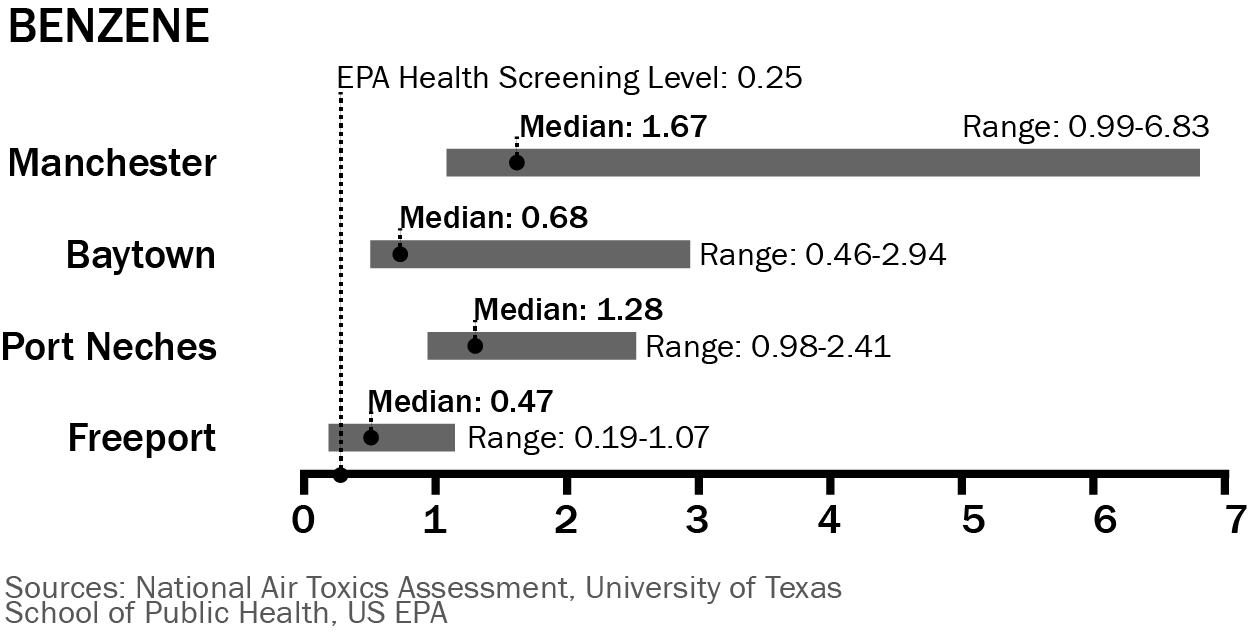
\includegraphics{images/HoustonChronicleWhatWeFoundBenzene.png}
    \caption{In all four of the neighborhoods the Chronicle monitored, the median concentrations
of Benzene were above the EPA's level where continual exposure
increased the detectable risk of cancer.}
    \end{figure}

    \begin{figure}
    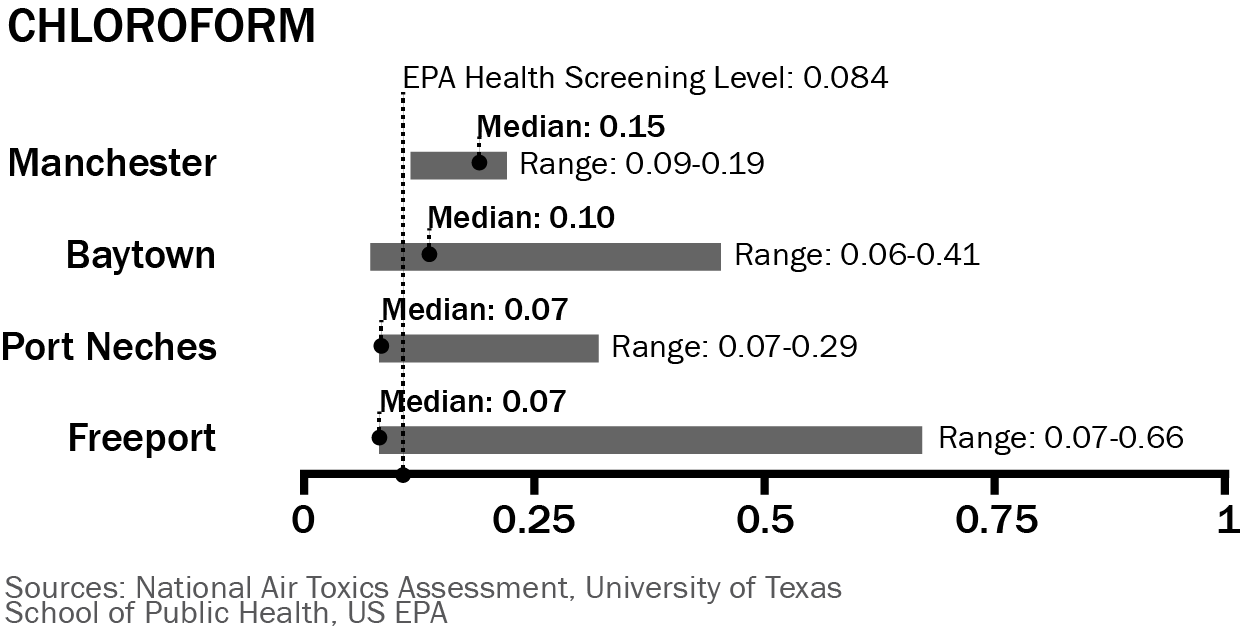
\includegraphics{images/HoustonChronicleWhatWeFoundChloroform.png}
    \caption{For Chloroform, two neighborhoods' median levels fell above the EPA risk
level, and two fell below although most of their ranges were above.}
    \end{figure}

    \begin{figure}
    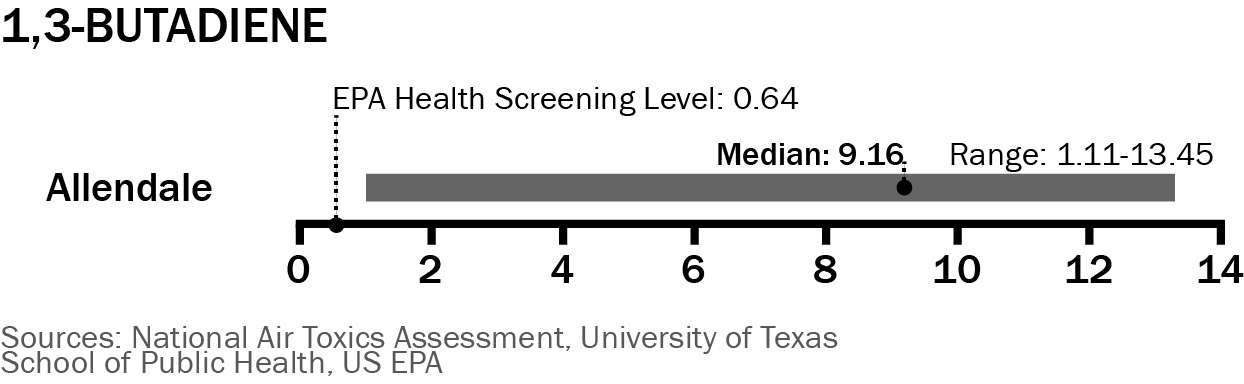
\includegraphics{images/HoustonChronicleWhatWeFoundButadiene.png}
    \caption{For 1,3-Butadiene in Allendale, the median was 14 times above the EPA’s
risk level.}
    \end{figure}

However, even though Cappiello’s results suggested that breathing the air in
the worst-affected neighborhoods was as harmful as breathing in air from
the New Jersey Turnpike, and often much worse than the EPA suggested is
healthy, it still fell within the legal limits for Texas, and within or below the
ranges recorded by the official monitors.

    \begin{figure}
    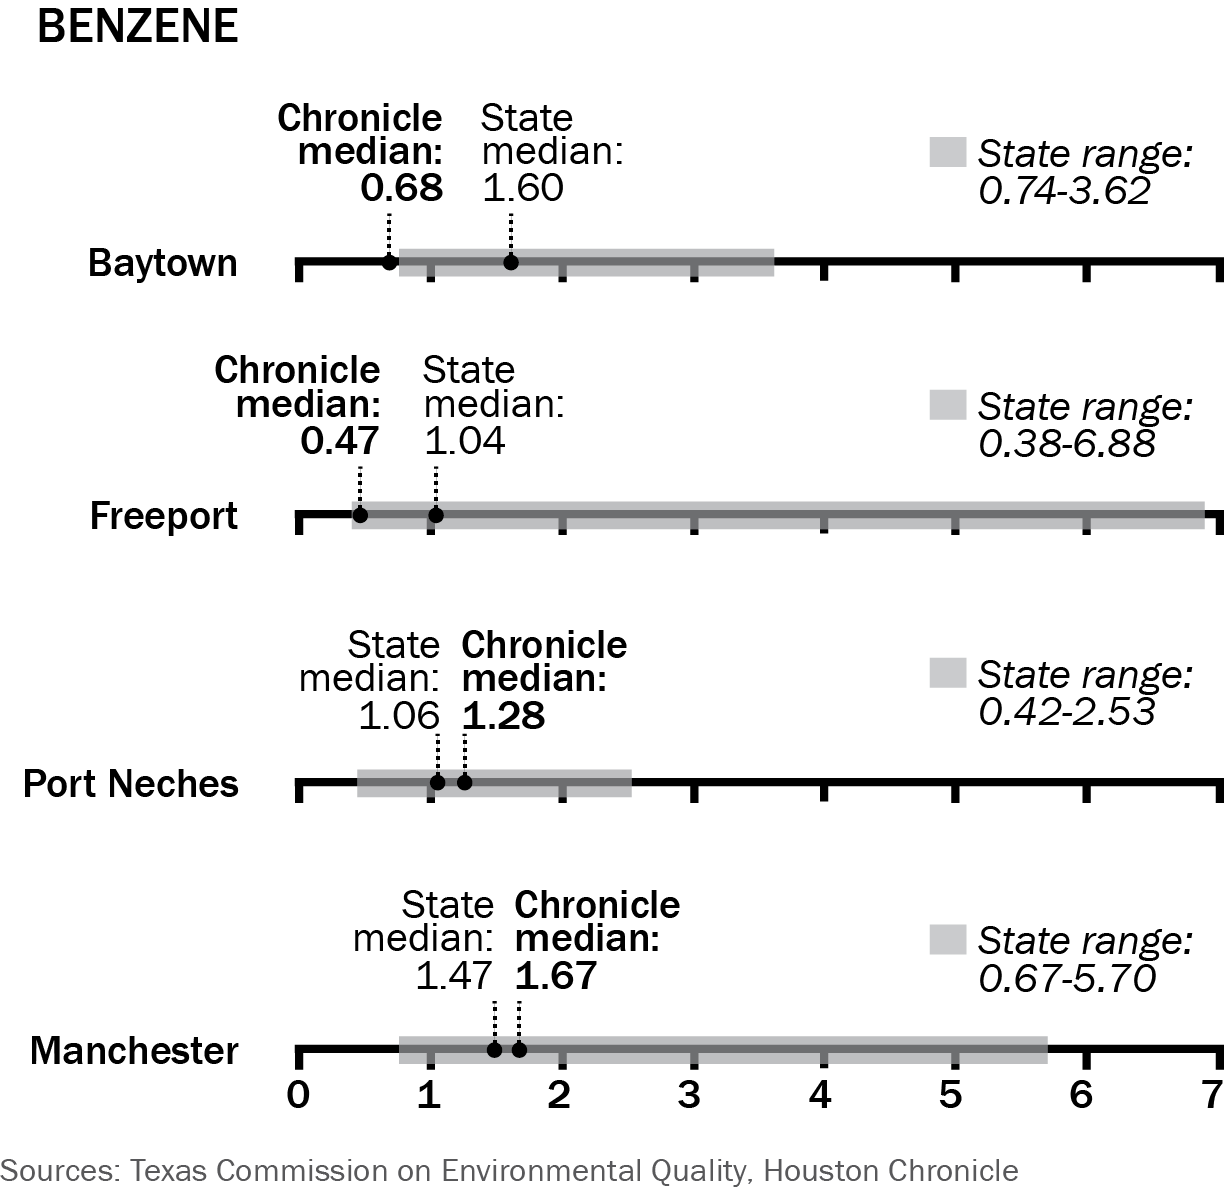
\includegraphics{images/HoustonChronicleBenzene.png}
    \end{figure}
    \begin{figure}
    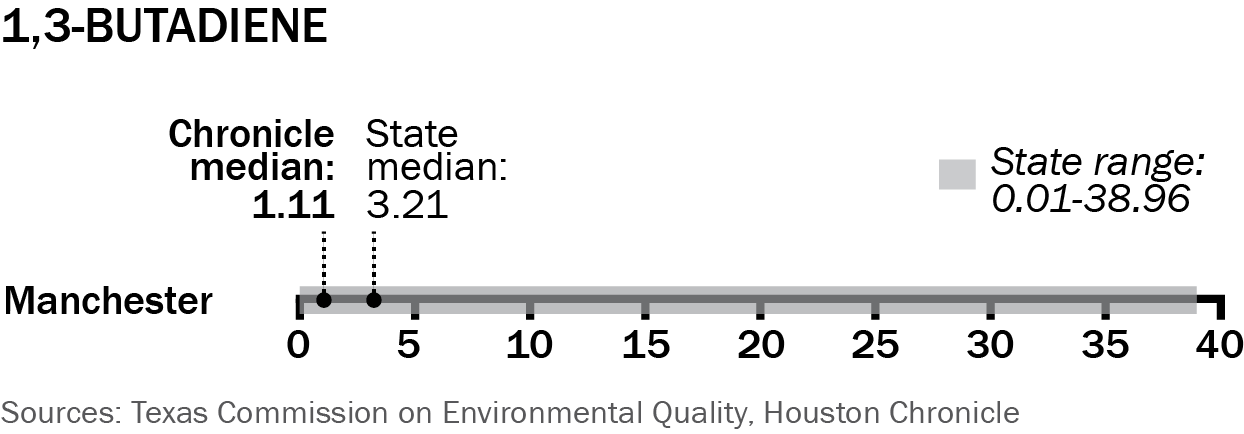
\includegraphics{images/HoustonChronicleButadiene.png}
    \end{figure}
    \begin{figure}
    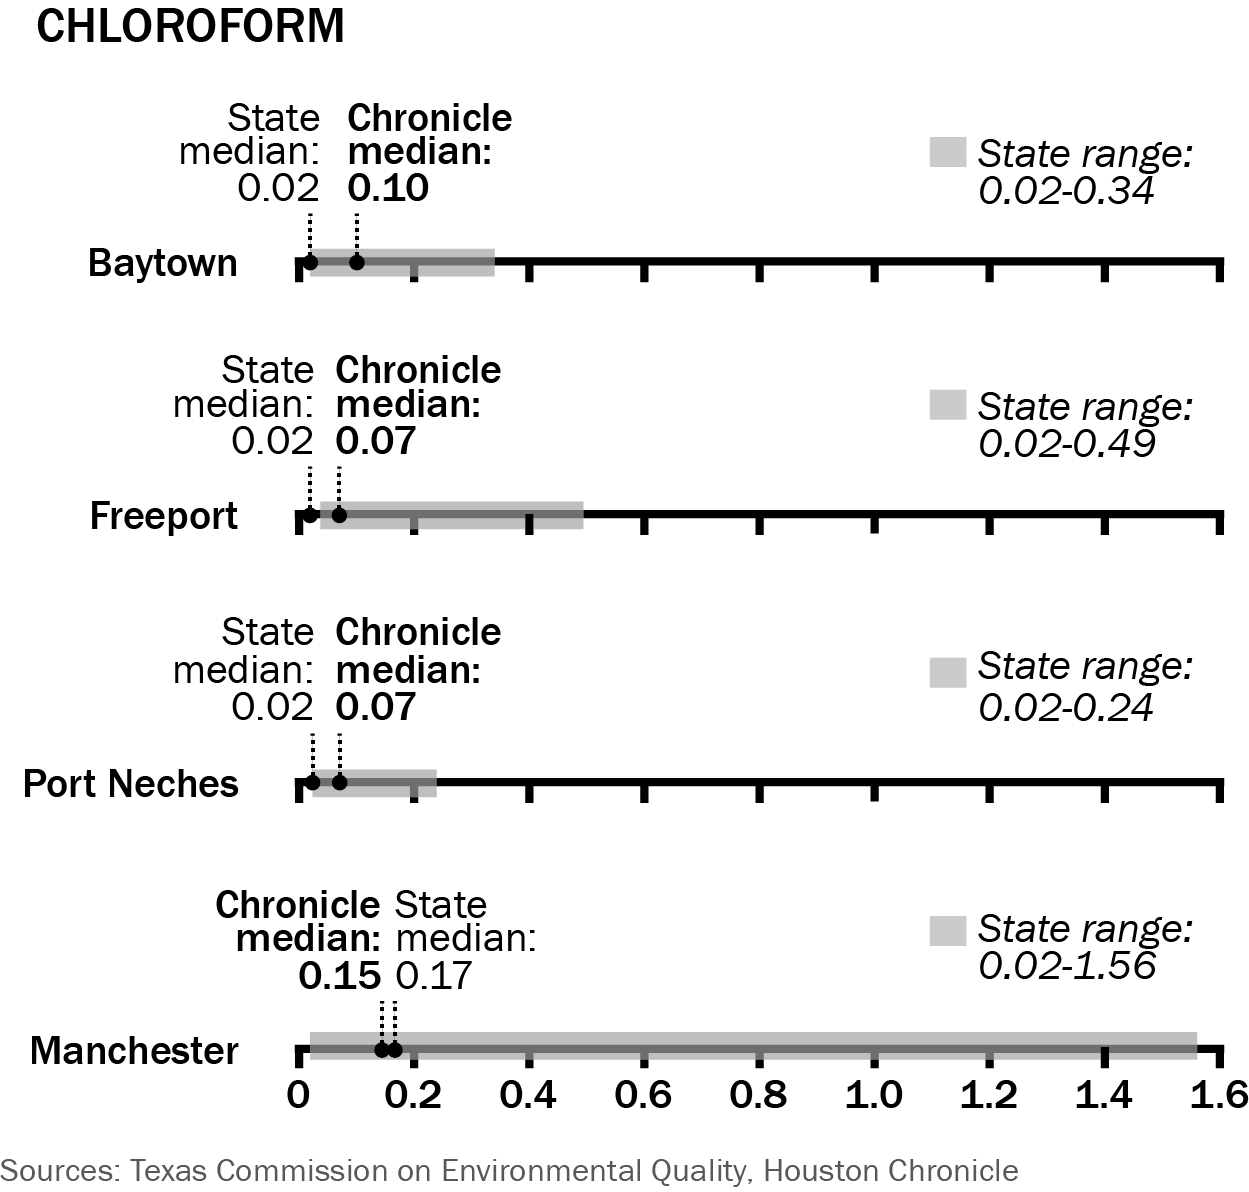
\includegraphics{images/HoustonChronicleChloroform.png}
    \end{figure}

Both Dina Cappiello and Dr. Thomas Stock agree that the methodology
the Houston Chronicle used was robust in the context of journalism, but
didn't approach the standard found in a peer-reviewed health sciences
journal. Cappiello acknowledges the critique that, for a high level of confidence,
testing should be done at least four times over the course of a year.
Likewise, Dr. Stock says the Chronicle's testing showed what was in the air in the neighborhood, but didn't incorporate indoor air quality—where residents breath some of the air that makes up their individual dosage of
harmful chemicals.

Dr. Stock says that the Chronicle's project did, however, raise awareness of
the problems in Houston's air quality in a way that academic studies rarely
do. In the weeks following publication, the mayor of Houston, Bill White,
funded a task force of experts to investigate Texas' air pollution and its
health effects. Its work became the basis of new academic study. Mayor
White also announced a plan to set up more air quality monitors in fenceline
communities. The Texas Petrochemicals company signed an agreement
with the city to reduce its butadiene emissions, and by December of 2005,
the Texas Commission on Environmental Quality had increased its air pollution
research and monitoring, especially along the fence lines.

The reporting project also had an impact in the journalism industry. Cappiello's
process inspired Blake Morrison of USA Today when he was planning
an investigation of the air quality around schools. Five years later, he used
the same organic vapor monitors as did the Houston Chronicle, supplementing
that data with active air-pump monitors and monitors which use
ultra-violet light to detect air contaminants.

In the 10 years since Cappiello's investigation, air quality has been a hot
political topic in Texas. The state's environmental regulators have continued
to set different standards from the federally operated EPA, and
that agency continues to bring cases against companies that release
hazardous chemicals.

\section{Distinctive and Notable}
\begin{itemize}
\item \textbf{This was non-electronic sensing.}

Dina Cappiello's data production method shares characteristics with
how contemporary sensing is understood. She deployed chemically
reactant badges, tools that recorded aspects of their environment and
could then yield information. The process extended human reporting
abilities by making the observations specific and quantified, and
allowed her to collect observations in many places simultaneously.
Electronics didn't come into the process until the badges were sent to
Dr. Thomas Stock's lab.
\item \textbf{The Chronicle's data was close to official data.}

The Houston Chronicle's initial hypothesis was that the official government
air pollution monitors were too spaced out, and in the wrong
places, to record dangers to the fence-line residents. While that may
have been true, the data Cappiello produced when she took readings
with a higher spatial density fell within the ranges produced by
the more spaced out, official monitoring stations. Furthermore, all
the sensors, government and journalistic, recorded levels of air pollution
that were within Texas' legal limits, even if they were higher
than other states' limits. However, the fresh set of data—evocatively
linked to individual people, whose faces and biographies the Houston
Chronicle showed—allowed the newspaper to kindle a debate about
whether the legal limits were safe and appropriate.
\item \textbf{The community's efforts were huge.}

Community management formed a significant part of Cappiello's
reporting process. She cultivated a contact who helped recruit volunteers
in Houston. She produced dual-language information sheets
and coached volunteers in the monitoring process. Throughout, she
remained aware that she was asking volunteers to help her produce
information that might have had significant consequences: lowering
the value of their homes and introducing health fears. Community
management appears to be a necessary skill common to other journalism
that incorporates environmental sensors.
\item \textbf{To avoid lengthy ``human subjects'' review, Dr. Stock's advice
had to be informal.}

When the Tow Center discussed the Houston Chronicle's project
with Dr. Stock, who advised Cappiello on how to use the monitoring
badges, he took pains to point out that his advice was informal.
If he had formally partnered with the Chronicle, he would have been
obliged to run the project through his university's ethical review process
for investigations concerning human subjects. Typically, human
subjects review processes take a number of months, can require training
for every team member who comes into contact with a volunteer,
includes a baseline assumption that all volunteers remain anonymous,
and that only team members named in the plan have access to their
data. The review processes are designed to ensure that research does
not harm participants. However, they are not set up to integrate with
the requirements of journalism and publishing.
\item \textbf{They hung monitors in public parks.}

The Houston Chronicle journalists made an assessment that they
didn't need to get permission to hang their monitor badges in public
parks. However, setting up monitors in public, unprotected locations
was not without its drawbacks: According to Cappiello, they did lose
``a couple'' of badges over the course of the project. The reporters,
one of whom was wearing a Muslim headscarf, also attracted the
attention of the FBI, which called Cappiello in response to reports of
suspicious activity.
\end{itemize}

\section{Lessons for the Industry}
\begin{itemize}
\item \textbf{Analyze other data sets to narrow down your investigation.}

Before deciding where to place her monitors, Cappiello inspected the
EPA's toxic releases inventory database. That helped her focus her
reporting on four particular neighborhoods.
\item \textbf{Assure volunteers access to the data.}

Cappiello ensured that the residents who hung monitoring badges
around their houses had access to the lab results once the badges had
been processed. Her decision to do so appears to anticipate the ethical
debates regarding data and access that have become more urgent
in subsequent years.
\item \textbf{Be advised that those affected by your data will want to know
the bad news.}

Cappiello, when contemplating what she was asking of volunteers,
realized that she could potentially produce data that threatened residents'
house prices or imply that they should move to protect their
family's health. If they worked in the refineries themselves, Cappiello's
story could cause problems for their employers. While some residents
refused to participate, many of her volunteers adopted the attitude
that if there was a problem, knowing about it would empower them.
\end{itemize}

\chapter{Public Lab – Homebrew Sensing}
The origin story of Public Lab, a non-profit community collective seeking
to investigate environmental concerns with DIY tools and techniques, is
deeply seeded in the BP oil spill off the coast of Louisiana in 2010. When an
explosion on April 20 sunk the Deepwater Horizon oil rig, killing 11 workers
and ripping open the undersea wellhead, the accident caused the biggest
oil spill in history. As the crude oil polluted the seawater and coastline, journalists
from across the United States and around the world flocked to report
the massive environmental story, threads of which were still making front
pages four years later. The story had traction for a number of reasons: Facts
and analysis were highly contested, information was selectively released and
journalists had to fight for access to the places where they wanted to report.

Some of the people at the core of today's Public Lab, Liz Barry, Jeff Warren,
and Shannon Dosemagen, were among the volunteers who rallied around
the Gulf Coast, helping with the cleanup and hoping to hold BP accountable.
They came at the task from various backgrounds in environmental activism,
innovative technology, and media and civic participation. Although none
identified as a journalist, they were trading in information and their motivations
approximated those of investigative reporters. In 2010 the group's
particular focus was working with local groups to record where the oil had
spread; a crucial piece of the puzzle in understanding how much damage
the spill would cause and how the cleanup money should be spent.

Since then, Public Lab has started to define itself, evolving into a community
aiming ``to change how people see the world in environmental, social,
and political terms.'' They encourage the use of inexpensive, accessible
equipment to collect information as a first step toward civic participation.
Around the Gulf Coast in 2010, this meant weather balloons, kites, and
cheap digital cameras. Later, it meant working with open source electronic
air and water quality sensors.

\subsection{Community and Journalism Innovation}
Public Lab's position in the news media landscape, however, is hard to define.
Although the word journalism doesn't appear in its mission statement and
its mailing lists attract more activists, engineers, scientists, and teachers
than they do reporters, as of April 2014, Public Lab has won \$850,000 from
the journalism and media innovation section of the Knight Foundation.^{\href{#endnotes-public-lab}{1}}
Those Knight News challenge awards account for about 55 percent of the
group's cash funding. Arguably, Public Lab fits within the new framework of
post-industrial journalism, where news-like information flows through
many publics and can take any number of routes to an audience. Some information
reaches audiences through mainstream media organizations, but
plenty more circulates on email lists, discussion boards and social media. A
co-founder of Public Lab, Shannon Dosemagen, told the Tow Center that
one of her current foci is to improve how Public Lab data can be used by civic
institutions, such as the courts and the legislative process.
For the purposes of this case study, to fully understand how Public Lab's
environmental sensing relates to journalism, it is necessary to understand
the Public Lab community itself. Jeffrey Warren, a co-founder and
the group's research director, says that when he introduces Public Lab to
someone he is meeting for the first time, his description shifts around:
He may say that Public Lab is a ``platform'' or ``a network of communities.''

A common thread in explanations of the organization is that Public Lab
avoids a top-down structure, or a singular drive toward a known outcome.
Public Lab's operations facilitate people meeting their own needs; often,
but not always, those needs concern environmental activism. However,
the organizers believe that if people are working in a connected way they
will have opportunities to learn from one another, share tools, and realize
unanticipated benefits.

\subsection{Aerial Mapping Versus Official Data}
In 2010, when oil was spilling out of Deepwater Horizon, those gnarly, high
concept questions were yet to be raised, let alone answered. In fact, Public
Lab didn't even exist. The activists' immediate concerns were twofold: In
the short-term they wanted to know where the oil was reaching the land,
so they could focus cleanup efforts. Later, that information might also feed
into an assessment of liability and damages.

At the time when the spill was at its worst, Louisiana authorities were
blocking photographers from accessing many parts of the shoreline. Airspace
restrictions also banned flyovers below 3,000 feet, an altitude too high
for news helicopters or planes to collect imagery with enough resolution to
show oil hitting the land.

Public Lab's methodology for documenting where the oil made landfall
combined elegance and scrappiness. They relied on an old, simple technology—
weather balloons and kites—hanging digital cameras to their craft,
stabilized with fins made out of plastic soda bottles. They floated the contraptions
above the shoreline, holding onto them with thin kite strings. As
the balloons flew, the digital cameras snapped photos under the control of
automatic timers, capturing images at pixel-per 3 cm resolution. After, they
pulled the balloons back in to retrieve the memory cards, loaded the files
into a specialized photo joining tool called Mapknitter, and stitched them
together to show stretches of coastline. The aerial photos showed black oil
stains at many points from just south of Lafayette, La., through to Perdido
Point, Ala.

One of the rationales for journalists producing their own data (using sensors
or any other method) is that official sources cannot always be trusted;
perhaps because they are incomplete, or they are wrong. Mat Lippincott,
who designs hardware for Public Lab, points to a particular case in Louisiana
where he says the official record of where the oil made landfall is wrong.
After the BP oil spill, the Emergency Response Management Agency
(ERMA) built a geographic database, rating oil pollution against a six-point
scale for dozens of coastal stretches from Louisiana to Florida. That database
became a source for maps published by The New York Times, the
Guardian, and plenty of other outlets. The official ERMA record, based on
its contractors' observations for July 22, 2010, says that in Wilkinson Bay, 20
miles south of New Orleans, floating boom-barriers kept the oil away from
the shore.^{\href{#endnotes-public-lab}{2}} By chance, the Louisiana Bucket Brigade, one of the local environmental
groups to which Dosemagan belongs, was also operating balloons
and kites in that location, on that day. Their photos show heavy oil
covering the reeds and marshes and broken booms that were intended to
block the oil from reaching land.^{\href{#endnotes-public-lab}{3}} (Although ERMA's underlying data might
be contested, no news media's maps we saw showed data at a high enough
resolution to see whether the inconsistency Lippincott cites was relevant or
included in their publishing.)

Balloon mapping has since become a common part of Public Lab's data collection.
They have used it to document sites of environmental conflict or
various ``occupy'' crowds.

\subsection{The Next Step: Tracing Source}
Later in 2010, the questions for Gulf Coast activists shifted from mapping
the spread of oil to establishing its source. Although at the time BP and local
governments were saying the cleanup was mostly complete, beach walkers
were still seeing tar balls and oil residue. BP's response was that the oil
could have been from any number of minor spills that happen throughout
the Gulf Coast.

According to Jeffrey Warren, the Public Lab people had no knowledge of
how to identify and fingerprint hydrocarbons. They started their research
in the typical way, by typing this question into Google: ``how to identify
oil,'' and the results that came back pointed them toward spectrometry—a
basic technique that has remained in use since its origins in the early 18th
century.

At its most basic level, spectrometry relies on the fact that different substances
absorb different amounts of colored light. After shining light
through a sample, the amounts that remain produce a signature that can be
compared to a catalogue of known samples. It is essentially a fingerprinting
process. Although various spectrometers have specific components that
allow the user to see the signature more clearly and do the comparisons
more aptly, the basic concepts remain consistent.

In the case of oil from the BP spill, the activists' theory was that they would
be able to take a sample of the black sludge on a beach, compare that sample's
signature to that of the known oil spilling from the Deepwater Horizon
accident, and show liability.

Perhaps unsurprisingly, that level of accuracy is hard to achieve, and in the
case of oil from the Deepwater Horizon Spill, did not get close oil spill.
Nonetheless, its idea of designing a low-cost spectrometer survived. Over
the next three and a half years, members of Public Lab have been producing
new versions of the hardware, all within the bounds of their underlying
DIY philosophy and design parameters. Today, they have two main designs: a small plastic version that clips on to the back of a smartphone and uses its
camera to record the spectra, and a larger ``desktop'' version, which incorporates
more people's design and development efforts. They aim for simple
construction and incorporate materials that are ubiquitously available. For
example, they use a section of DVD as their diffraction lens and their desktop
version uses a standard household plumbing conduit as its body.

\subection{The Open Source Hardware Approach}
Although the original demand for the spectrometer was the Gulf Coast
spill, Public Lab's philosophy is to support whatever application their community
finds for their equipment. Josh McIlvain, who completed a physics
undergraduate degree from Kansas State University, used the spectrometer
to analyze the components of laundry detergent, detecting dyes in a
supposedly ``free and clear'' brand. Environmental activists who suspected
their local Louisiana industrial plants were releasing harmful contaminants
have developed a plan to use the spectrometer to analyze flares from an oil
refinery and a lubricant factory. But mostly, the uses shown on Public Lab's
community upload section tend toward experimentation and exploration.

Public Lab's approach has been successful in attracting funding: It ran a
Kickstarter campaign in 2012 to improve its DIY Spectrometry Kit and
raised \$110,538, 11 times its \$10,000 goal. In the Knight News Health Challenge
of 2013, Public Lab won \$350,000 for its Homebrew Sensing Project.
The pitch to the Knight Foundation paints a picture of a decentralized
network of contributors using citizen science approaches to document and
address ``environmental health threats and their impacts.''
Public Lab's open operating model extends beyond facilitating unanticipated
uses of its hardware. It also supports community members' development
of their own equipment. One such example is a prototype called
``The Riffle,'' an electronic water sensor designed to be deposited in a stream
to collect data on water quality and pollution. The device designers, Ben

Gamari and Don Blair, are both fifth-year biophysics Ph.D. candidates at the
University of Massachusetts, although this work is not part of their formal
study. The current prototype of the Riffle logs temperature, water pressure,
and conductivity, which can be broad indicators of abnormal activity; especially
high levels of agricultural fertilizer runoff or releases from industrial
plants. While those measurements are basic, Gamari and Blair say that they
want to make it viable for citizens to continuously monitor water quality
at very low cost. The Riffle is designed to use mostly household plumbing
parts and cheaply available Arduino-based electronics, although one specialist
component needs 3D printing, a production method that they hope
will become increasingly mainstream.

    \begin{figure}
    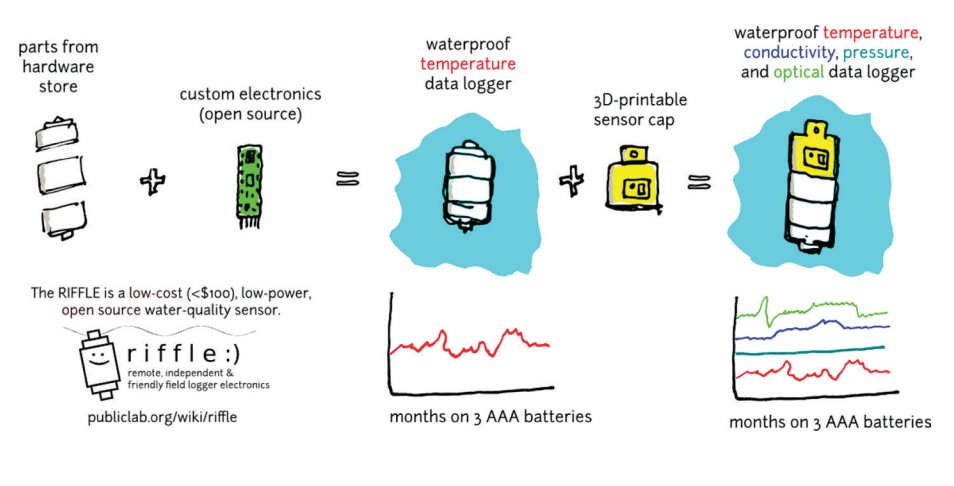
\includegraphics{images/PublicLabRiffle.jpg}
    \end{figure}

Since winning the Knight News Challenge in 2013, Public Lab has picked up
more philanthropic funding, some for basic operations and some for specific
issue-based campaigns. The Schmidt Family Foundation has funded
Public Lab to work with Wisconsin residents and monitor air quality around
frac-sand mining, a production process that can send fine-grained particles
into the air and put citizens at risk for respiratory problems and possibly
lung cancer.

\subsection{The Challenge for Citizen Science, and the Roadmap}
However, Public Lab's work, especially its spectrometry and electronic
sensing, does attract skepticism. In comparison to lab-grade equipment,
Public Lab's current hardware is extremely immature, and while it does
produce data, it is not clear whether that data can be compared to known
health or regulatory standards to the degree that would stand up in court or
withstand a contest from polluters. Likewise, the spectrometer's sensitivity,
precision, and range are yet to meet the requirements of measuring samples
with the kinds of pollution concentrations found in many real world environmental
situations.

Dr. John Feighery, an environmental engineer who consults for the World
Health Organizataion and UNICEF on water quality and managed the
development of water monitoring hardware for NASA's International Space
Station, describes the difficulties in Public Lab's spectrometry use. 
\begin{quote}
``The
challenge in water analysis is both detecting very low levels and with a large
number of other compounds present. These are the typical conditions in
environmental samples. If you think of the spectra of one compound as
like a fingerprint, then imagine dozens of very faint fingerprints all on top
of each other on the same spot, you start to get the picture.'' 
\end{quote}
Until Public Lab can produce data showing detection of a contaminant of interest in a
realistic environmental sample, Dr. Feighery says he will remain skeptical.
He told the Tow Center, however, that he admires Public Lab's work, but
thinks its current spectrometer development seems more like a hobby than
a practical device for fieldwork.

Jeffrey Warren is aware of experts' reservations, and his response to it hinges
on the idea that Public Lab's activity does not have the kind of singular goal
to which scientists or journalists are accustomed.
\begin{quote}
``We talked a lot about this early on in the founding of Public Lab. A
lot of people asked, 'Are you focused on the benefits of people being
involved in the process, where the involvement itself is a transforma
tive approach to creating environmental science, or are you focused
on the outputs: the things you can prove, the legal decisions you can
influence, the regulations that you can enforce? Or, are you interested
in the media attention that you can generate?' And I know it's
not a satisfying answer, but the answer is, \'All of the above.\'''

``For us to have a citizenry that is capable of affecting change through
the collection of data, through the advocacy based on that data,
through the strong, productive relationships with government and
even industry, they're going to need to be involved in the process
in more than a token way. They're going to need to learn about
the techniques.''
\end{quote}

Other people within the Public Lab community say that their hardware
development process, if given time, should show good results, and cite the
open source software movement as an example of how tools' quality and
utility can be built over the long term. The Riffle designers, Gamari and
Blair, who use the open source programing language Python in their labs,
say the goals for their water quality sensors have always drawn on that experience.
Blair says, ``Part of the vision is having something like [open source
software community] Stack Overflow for all of the instrumentation that
people are using in science.''

\section{Distinctive and Notable}
\begin{itemize}
\item \textbf{There's activism, then there's journalism.}

The Tow Center has included Public Lab in this report largely as a
result of the funding it has won from the Knight News Challenges.
While its founders don't self-identify as reporters and their activity
looks nothing like traditional journalism; they don't write mainstream
news stories, make video programs or broadcast radio shows, many
people in the Public Lab community appear to share motivations
with journalists—to uncover information and put it to use in the civic
space. Mainstream media lost its monopoly over the means of media
production, publication, and distribution years ago. One result is that
the distinctions have blurred between journalism and everything else.
Public Lab's activities are a case in point.
\item \textbf{Data utility, and how data accuracy informs it.}

Public Lab projects produce data with highly variable utility. Their
aerial mapping techniques can produce photographic evidence that is
reliable and believable. For journalists, these techniques may be useful
as a source of content and data that is alternative or additional to official
sources, especially while drones are unsafe, illegal, or impractical.
Their other hardware projects, the spectrometers, the Riffle, and the
near infrared cameras, are yet to produce data meeting a standard of
accuracy where it can be compared to legal limits or health standards.
For journalists who are working on investigative projects or stories
where an issue is environmental safety and legality, the immaturity
of Public Lab's tools should give pause. However, Public Lab members
say that the data they produce still has value as an early warning
that better monitoring is needed, or to make illustrations that attract
media and public attention. They also say that the very act of participating
in data collection educates and engages a citizenry to become
environmentally concerned and politically active.
\item \textbf{Newsrooms could frame Public Lab content as the UGC of data.}

Progressive newsrooms have become increasingly sophisticated in
how they incorporate user-generated photos and videos into their
journalism. In broad terms, attitudes evolved from a lack of interest,
to suspicion, through enthusiasm to judiciousness. Big news companies
such as the BBC have verification regimes and the startup company
Storyful built a \$25 million business on providing that service to
many newsrooms. So far, we're not aware of any newsrooms incorporating
community-produced environmental sensor data into their
UGC harvesting. This may be an opportunity.
\item \textbf{Public Lab has engaged the maker movement.}

On its mailing lists and wikis, Public Lab hosts skilled electronics
enthusiasts who are keen to use their abilities to contribute to a common
good. They design hardware, test prototypes, give feedback, and
suggest developments. This appears to be a positive example of makers
investing what writer and Internet theorist Clay Shirky calls ``cognitive
surplus.'' That degree of engagement has built Wikipedia and
released masses of valuable open source software. It has shown itself
to have huge potential. Indeed, the hardware development process
apparent in Public Lab borrows a lot from the open source software
development movement. In early stages, open source software projects
tend to be unusable and unreliable, only to evolve into excellent,
widely used products. Participants in Public Lab's projects express the
hope that their hardware projects will follow the same path.
\item \textbf{Public Lab's work crosses into many fields attracting skepticism.}

Public Lab, being a complex, multifaceted organization, does things
that look a bit like science and engineering (experiments and data collection)
and a bit like journalism (producing and distributing politically
potent information). Practitioners in those fields apply their own
traditional values like accuracy and verifiability when assessing Public
Lab's activity. While Public Lab's people recognize those values,
thus far they appear to have prioritized accessibility and community
engagement.
\item \textbf{Open source hardware development is behind open software.}

When compared to the breadth, depth, and maturity of open source
software, open source hardware appears quite infant. While the tools
and ecosystem supporting open source hardware have developed
a great deal in recent years (the case study examining the WNYC
Cicada Tracker goes into more detail on the subject), some headwinds
remain. Whereas a new open source software build is generally
free (apart from minimal computing resources), whenever an opensource hardware project moves from design to build, even as a test,
it requires physical resources. The tools always have a hardware cost,
and even though those costs have dropped, they remain significantly
above zero.
\end{itemize}
\section{Lessons for the Industry}
\begin{itemize}
\item Engagement needs benefit.
Public Lab has, in just four years, built a very large community of
people, some of whom have contributed large amounts of effort for
no payment. Crucial to that degree of engagement is that individuals'
participation delivers them some kind of benefit—learning new skills,
being heard in a debate, affecting civic processes, uncovering information
about their local environment, etc. Public Lab's practice of
eschewing top-down control in favor of self-determination undoubtedly
helps with that. Many media organizations include engagement
in their objectives, but few are able to release as much control as has
Public Lab and are often focused on the benefit the company gets
from participation, as opposed to the community.
\item As a journalist, beware that official data may be contestable.
The processes that produce official data can be complex, opaque, and
ridden with errors. In the case of data describing where oil from the
Deepwater Horizon made landfall, the production was contracted and
subcontracted. At the first stage of the production chain were people
on boats, working in a difficult environment, using a newly implemented
process. However, those messy, human production processes
are rarely brought to journalists' attention when the data is supplied.
\end{itemize}

\chapter{USA Today—Ghost Factories}
Alison Young says she is a junkie for lead smelters. She follows that up with
a chuckle, but given her track record, it is probably a fair label. It is also a
characteristic that has won her numerous journalism awards and underpins
pollution watchdog stories she has reported for four different newspapers
over 13 years.

Over that time, as the techniques and technology of journalism evolved,
Young's reporting has incorporated more and more environmental data
collection. Her ambitious project, USA Today's ``Ghost Factories,'' saw
reporters take more than 800 field tests of suspect soil and prompted the
US Environmental Protection Agency (EPA) and state environmental agencies
to launch new cleanup efforts.

Young wrote her first report about the toxic remains of a lead smelter while
she was working for the Dallas Times Herald in 1989. Despite the EPA's
claim that the site was clean, the soil in the area still held large amounts of
lead—a contaminant linked to kidney damage, heart problems, and slow IQ
development in children.

Twelve years later, working at the Detroit Free Press, Young edited a series of
investigations into lead poisoning from gasoline and old industrial plants. A
group of reporters, led by Tina Lam, published a story about the contaminated
Master Metals factory site just north of Detroit midtown. At the time,
in 2003, they outsourced the soil sampling to one of the country's leading
experts in soil contamination, Dr. Howard Mielke.

Around that time, very little attention was being paid to a study published
by Dr. William Eckel in a 2001 edition of The American Journal of Public
Health. He wrote that up to 430 old metal working factories had been closed
and forgotten, potentially leaving behind heavy metal poisons at the sites
and in surrounding neighborhoods. The families that moved into the areas
had no way of knowing that their children could be playing in unsafe soil.
But the study found its way to Young. ``I have always done a lot of reporting
in the area of public health and environmental health and so one of the first
things I tend to do is a search of the scientific literature,'' she says.
In October of 2009, working in Atlanta, Young again pulled out Eckel's list
of forgotten industrial sites. Just before she left The Atlanta Journal-Constitution
she wrote a story about the old Evans Metal Company, a lead factory
that had been shut down, sold, and redeveloped with no EPA oversight to
ensure the plant's land and its surrounds were clean.

So when Young arrived in USA Today's investigative unit in November of
2010, she was primed to do a nationwide investigation based on Eckel's
list of old smelter sites. Blake Morrison, the editor of the new investigative
team, was a longtime reporter at USA Today and had worked on a series
called ``Smokestack Nation,'' which had included air pollution sampling
techniques pioneered by The Houston Chronicle (which are discussed in an
earlier case study of this report).

From the outset, Young and Morrison anticipated that their investigation
would need to include soil testing, but Young expected they'd need to outsource
the work to Dr. Howard Mielke, as she had at the Detroit Free Press.
However, while Young was in her research phase, reading the academic literature
and government reports, the papers' authors kept referring to a new
device: the X-Ray Fluorescence (XRF) analyzer. Handheld XRF analyzers
look a bit like a ray gun from a sci-fi cartoon. They shoot x-ray beams into a
sample, pumping energy into the atoms. Each substance's electrons absorb
and lose energy at different rates, throwing light back to the XRF analyzer
at characteristic wavelengths. An onboard sensor detects the emissions and

compares them to a library of known patterns, logs the data, and shows
the results on a small display. The fact that so many different people were
using these new tools hinted to Young that the reporters could do some of
the data collection themselves, bypassing the huge expense of outsourcing
the sampling and increasing the amount of data they could collect, economically
speaking. Hiring outside experts to take field samples nationwide
would have been incredibly expensive. Typically a newspaper would have to
pay consultant rates for multiple scientists to travel to each location, take
soil samples, and then do the processing back at their lab.
A company called Thermo Fisher made a leading line of XRF analyzers, used
in the fields of environmental regulation, resource mining, and industrial
production. Although Young hadn't seen any examples of journalists using
them, the tools appeared to be relatively easy to operate. ``Blake Morrison
was saying, 'Well, what if we could?' '' says Young. ``That's a very important
thing when you're trying to do something that hadn't been done before.''
Although the upfront purchase cost would have been \$41,000 per unit,
Morrison was able to negotiate a rental agreement of \$2,250 per device, per
month. Still, having worked in health and science reporting for a long time,
Young knew that their process had to be valid. ``If we can't do it right, we put
any journalism we do at risk.''

\subsection{Developing the Methodology}
Alison Young consulted Dr. Mielke to help her develop their reporting plan.
``It's not enough to have the tools, or the sensors. Just like in database journalism,
if you don't ask the right question, you're going to get garbage back,''
she says. ``If you go out into the field and start testing without a valid plan,
you're also going to get garbage.''

Young's project was different from the types of randomized field studies
that health researchers like Dr. Mielke normally conducted. His teams were
used to looking for problem areas across a whole community. Meanwhile, health authorities' studies were often designed to understand the total
cleanup costs. In contrast, Young's project would test her hypothesis that
the contamination from old lead factories fell on the soil in particular locations—
putting families at risk.

Young drafted her sampling plans and sent them to Dr. Mielke, who helped
her assess whether her protocol would produce the data to answer her question.
The final plans dictated that the reporters take their samples within a
mile of the old factory sites, mostly in the direction of the prevailing winds.
They reviewed aerial photographs to avoid confounding factors like current
industrial plants and locate soil that likely hadn't been disturbed—mostly
bare grass in backyards.

The XRF analyzer USA Today used was designed for field sampling. It's selfcontained,
it self-calibrates, and has onboard software to stop users tampering
with the data—a feature put in place to meet the standard for regulatory
use. But industrial clients also use the devices to check that the steel parts
they receive match the chemical specifications they have paid for. Miners
use the device to analyze soil. Workers across all these different industrial
applications set the units with subtly varying settings. As part of the rental
contract, the tool's manufacturer, Thermo Fisher, set the units to analyze
soil for specific pollutants for USA Today.

``Originally, we were going to report on arsenic and a variety of other compounds
in the soil,'' says Young. ``For simplicity's sake [in] explaining to readers,
we just stuck with the lead, but we wanted to be able to capture as much
data as possible, in case we needed or wanted it later.'' USA Today also contracted
Thermo Fisher to send training videos and instructors to provide
hands-on instruction for Young, her co-reporter Peter Eisler, and a backup
reporter in case Young or Eisler got sick.

\subsection{The Reporting}
When Alison Young and Peter Eisler got into the field, they were carrying the
XRF analyzers, their field notes, cameras, and microphones to produce the
video they wanted. The reporters also had legal releases and documents for
the residents living on the property where they took most of their samples.
The releases informed the residents that their exact street addresses wouldn't
be published and that their names wouldn't be used unless they specifically
agreed. Dr. Mielke had suggested USA Today write up information sheets
to leave behind for the homeowners, who suddenly had to absorb the possibility
that the soil in their backyard might be harming their children. The
leave-behind information packs gave the residents the results of the tests for
their backyard, along with contact details for local environmental agencies,
regulators, and some resources to find out more information.

In backyards, public schools, and sports grounds the reporters took more
than 800 surface samples with the XRF analyzer and collected around 190
additional samples of earth to send to Mielke's lab at Tulane University for
more exhaustive analysis. Young and Eisler were on the road for almost two
full months. The expensive lab tests performed at Tulane correlated with
the recently trained journalists' field sample results.

The field tests ``revealed potentially dangerous lead levels in parts of all 21
neighborhoods examined across 13 states.''^{\href{#endnotes-usa-today}{1}} Although the EPA says that 400
parts per million (p.p.m.) is the upper safe amount of lead in soil where children
play, states set their own regulatory limits. For example California's
limit was 80 p.p.m., whereas New York's was 400 p.p.m.

Tests that Young and Eisler performed using the XRF analyzer ``showed several
neighborhoods had lead levels greater than 2,000 p.p.m., topping 3,400
p.p.m. in Cleveland, Ohio; Portland, Ore.; and Carteret, N.J.'' A baseball field
in Red Hook, N.Y., showed lead levels of 2,000 p.p.m. When USA Today
informed city officials, they shut the park down until the fields could be
resurfaced. Six out of 16 tests performed in nearby public housing yards
showed levels over 400 p.p.m.

Young and Eisler's story documented neighborhoods in Philadelphia where
children were playing in soil with lead concentrations more than double the
EPA's limit. Although blood testing was not part of USA Today's reporting
plan, parents living in a contaminated Philadelphia neighborhood had their
child tested, and found a blood lead level of 0.075 milligrams per liter, a
concentration ``associated with decreased IQ and an increased incidence of
ADHD and other issues, medical studies show.''^{\href{#endnotes-usa-today}{2}} In many places where the
reporters found dangerous pollution, Young had evidence that the EPA had
either gone looking for the closed factories documented on Eckel's list, but
failed to find what USA Today did, or knew there were risks and took no
actions. Many state environmental agencies were similarly ineffective.

\subsection{Publishing}
Although the data from the soil tests was crucial to USA Today's finished
story, the newspaper company's online publication in April of 2012 took the
form of an extensive multimedia presentation. Aside from many thousands
of words, it included video segments, photos, embedded government documents,
and an index of the sites on Eckel's list with map overlays showing
historical plans of the factories and the soil sample data from the reporters'
testing. USA Today staff hand-positioned its data markers on the map so
that the pins didn't fall directly on houses where residents had elected to
keep their addresses private.

Young says that after publication they took phone calls from state regulators,
who pointed out that they hadn't followed the randomized process
the regulators used to start enforcement procedures. Young's response, she
says, was that USA Today had produced enough reliable information to
show that even though William Eckel's study had pointed to neighborhoods
where old smelter sites posed a high risk of poisoned soil, the regulators
didn't know whether the land was safe and there was enough data to suggest
they should find out.

Mielke used the term ``screening'' to describe the utility of USA Today's
data. He says that, as a first pass, it produced reliable enough evidence to
suggest environmental regulators should invest the extra resources to procure
legally sound data in preparation for a cleanup.

After USA Today's first publication, the journalists continued to report on
the series' impact. In Carteret, N.J., the local government reached an agreement
with the owner of a closed factory, who would pay \$1 million to assess
and clean up the surrounding area. In Portland, Ore., the EPA agreed to pay
for cleanups at five homes the reporters had tested, and committed to testing
at a sixth. The EPA inspector general, who was responsible for auditing
the agency's operations, prioritized a review of its performance in reducing
health risks from old lead smelters. U.S. senators from New Jersey, Ohio,
Pennsylvania, Rhode Island, Oregon, and Minnesota pressured the EPA to
take immediate action, review all the sites, and set priorities for remediation.
In November of 2012 the EPA announced it would reexamine 460 former
lead factory sites. However, Alison Young says the testing and cleanup
actions from national and state environmental agencies were uneven. When
she asked state regulators, before and after USA Today published in April,
why they hadn't tested, the answers were always about lack of funding: ``Literally,
one of them said to me, 'because if we do, and if we find something,
then we have to do something, and we don't have the money.' ''

\section{Distinctive and Notable}
\begin{itemize}
\item \textbf{Dr. Eckel's paper had been available for 11 years when
USA Today published.}

The newsworthiness of Dr. Eckel's paper identifying 430 forgotten,
potentially toxic smelter sites evolved and grew over the 11 years
between its original publication in 2001 and USA Today's report in
2012. Initially, the story was simply that these sites existed and environmental
agencies likely needed to take action. Over time, it shifted
to outlining that these sites, probably toxic, were now known, and
environmental agencies were continuing to take no action even
though public health was probably at risk. That lack of action became
less excusable as time passed. USA Today's story demonstrated that
the risks were real and relatively easy to confirm.
\item \textbf{The development of XRF analysers opened up new
reporting opportunities.}

Although environmental testing was a known investigative technique
before this story was reported, the advent of a rentable electronic,
self-contained devices that journalists could learn to operate meant
USA Today could take hundreds more samples than was previously
economically viable.
\item \textbf{The journalistic hypothesis required a different
sampling approach.}

The differences between Alison Young's goals and other applications
of soil testing came into play at two main points in USA Today's project.
When she was designing her testing process, she was trying to
verify whether a particular pollution source was endangering particular
residents. She therefore could not use a template from a health
researcher's project where the goal was to get a representative sample
from a large area. When USA Today published, according to Young,
experts who worked in environmental agencies said that her process
was not the same one they would use to plan and estimate the cost of
a cleanup and suggested her story was therefore invalid. That tension
appears to be the result of practitioners from two different fields using
similar processes for different ends.

\item \textbf{Having an adventurous editor helped.}
Young suggested a reporting process incorporating XRF analysers,
which journalists had not used before. That entailed risks. However,
her editor, Blake Morrison, had previously used sampling while
reporting on his own large environmental projects with some success,
and supported Young's concept.
\item \textbf{Health authorities, experts, and states do not agree
on standards.}

Part of the impact of ``Ghost Factories'' came from its hard, quantified
data. The reporters were able to produce numbers that were ripe for
comparison. However, there was room for debate about how to compare
their data. Although some of their soil samples had lead concentrations
above 2,000 p.p.m., which were clearly unsafe for children's
play areas, many samples had lead concentrations in the hundreds of
parts per million. USA Today emphasized the EPA's 400 p.p.m. in its
presentation, but also noted that California set its limit at 80 p.p.m.
In later stories, Young wrote that many experts believed that a 400
p.p.m. limit for children's play areas was too high.
Lessons for the Industry
\item \textbf{Without good technique, the technology won't help.}

When the Tow Center spoke to her, Alison Young repeatedly emphasized
that the newly available XRF analysers could have easily produced
useless data. Alternatively, the data they did produce could
have been interpreted incorrectly. Two factors gave strength to her
findings. First, she had a clear hypothesis that could feasibly be tested
using the technology. Second, the reporters developed a testing protocol,
with input and review by an expert in the field who helped
ensure it had rigor and validity.
\item \textbf{Initial research reduces the risk of finding nothing.}

By the time Young and Morrison made their pitch to USA Today's
senior editors, asking them to approve an extensive reporting process
and a large cash spend, they had filed FOIAs for EPA documents,
knew the dominant wind directions that would influence the most
likely problem spots, had read the scientific literature—all on top of
Young's long experience covering similar stories. This offered their
editors confidence that there was probably a story to be reported, and
that evidence could be collected to write it.
\item \textbf{Make privacy a high priority.}

Many of the residents who allowed USA Today to sample the dirt in
their yards wanted to remain anonymous. The journalists needed to
respect their privacy while still showing relevant results on a map. So,
USA Today staff, having initially placed the map pins based on residents'
street addresses in an automated fashion, had to move the pins
manually onto nearby median strips and public space.
\item \textbf{Prepare leave-behinds to help your sources understand
your findings.}

Dr. Howard Mielke, a research professor with long experience doing
environmental testing in residential areas, advised Young to prepare
for situations in which the people whose yards she tested would want
help understanding the data she had just produced. Understandably,
he anticipated that they would probably be overwhelmed: This was
important information with serious implications, and in contrast to
the reporters who had been immersed in the data for many months,
there was no guarantee that the residents would be familiar with lead
pollution and its health effects. However, while the reporters could
supply the specific data they found and some basic background, for
more information or to take action the sheets pointed the residents
toward health and environmental agencies.
\item \textbf{Be prepared for non-technical reporting obstacles, like
language barriers.}

Outside of technical sensor use, Young says she wishes she had developed
a plan to deal with the language barrier her team encountered.
While they had prepared for all kinds of testing, their inability to
speak languages other than English in some neighborhoods limited
the testing they could do.
\end{itemize}

\chapter{Sun Sentinel – Above the Law}
For police officers in many Floridian cities, a longstanding perk of their jobs
is a take-home car—even relatively junior officers get one. The benefit offsets
the job's low public sector wages and the dangers of duty, police unions
argue, while attracting recruits and keeping them in the force.^{\href{#endnotes-sun-sentinel}{1}}
But before Sally Kestin and John Maines from the Sun Sentinel in Fort Lauderdale
wrote their Pulitzer Prize-winning stories about speeding police
officers, Florida's cops were driving thousands and thousands of trips at
more than 30 m.p.h. above the speed limit; breaking the law, causing fatal
accidents, and escaping heavy penalties.

The reporters' work eventually forced the police departments of Miami,
Fort Lauderdale, and eight other state police departments to launch internal
affairs investigations cracking down on speeding cops. Follow-up reporting
showed that the series shifted the police culture from one of blatant disregard
to safer compliance.

What Kestin and Maine's reporting produced is a story in which sensor data
revealed a secret culture of police disregard. While outliers and special cases
were crucial to give the narrative bite, they weren't at its heart. Though the
duo didn't necessarily set out to combine sensors with data analytics and
investigative reporting, these are their story's driving forces.

Through 2010 and 2011, Sally Kestin says Floridians were well aware that
their off-duty police were smashing speed limits along the expressways. One
of Kestin's readers would call to bemoan that he always saw cops ``speeding
like crazy'' on his daily commute.

When Fausto Lopez, a Miami police officer, sped past trooper Donna Jane
Watts' car on October 11, 2011, he was clocked driving his marked police
car at 120 m.p.h. in a 65 m.p.h. zone. Trooper Watts accelerated to chase
Lopez and pull him over but the officer wouldn't stop. The video from
Watts' dash-mounted camera shows Lopez speeding away for eight minutes
before finally acknowledging Watts' commands. When the story and
the video become public, newspaper editorials and social media erupted.

But the problem remained: how to debunk the Floridian police departments'
standard defense that Lopez—and perhaps a couple of other cops—
were merely a few bad apples. The Sun Sentinel wanted to show that while
Lopez was certainly an extreme example, he wasn't such a radical outlier.

Mid-November of 2011 found John Maines and Sally Kestin standing in the
rain by an overpass above Florida's Turnpike, pointing a speed gun they'd
just bought at cars as they whizzed through the narrow strip of suburbia
that separates the Everglades from the beaches above Fort Lauderdale. In
the most optimistic scenario, it was conceivable that the reporters would be
able to collect a few hundred speed readings, enough data to expand their
own picture of speeding cops from just a handful to the low hundreds. But,
as investigative reporters, they quickly understood that their data would be
highly contestable: Police and other skeptics could argue convincingly that
the equipment wasn't reliable or that Kestin and Maines couldn't be trusted
to operate it properly. The data would not be reproducible. The two journalists
asked police departments for data from the GPS units that tracked
the location of police-owned cars, but the departments said delivering that
information constituted a security risk to officers who parked their cars in
their home driveways.

Once again, it was a reader who called to complain about police speeding
that helped Kestin move the investigation along. The reader mentioned the
tollgate data from the expressway. ``'Well, you know SunPass has these dates
and times,''' Kestin reports the reader saying. ``So that's how it originally
came up—in a conversation with him,'' she says.

The data reporting for this project was only possible because Florida had
built connected, physical sensing systems that could accommodate the
complexities of the bureaucracy's financial transactions. Florida police were
not only entitled to take-home cars, but those cars were allowed to travel
for free on the state's tollways. However, the highly automated world of
SunPass still needed to know that the car passing through the tollgate was
legitimately not paying. Theoretically, the police cars could pass through,
be photographed, and SunPass employees could check the number plate
against a registration database, conclude that it was a police-owned car, and
drop the fee. But that would be a wasteful process. So the police attached a
standard SunPass RFID transponder to each state-owned car. In SunPass'
back-office systems, all of the police's transponder IDs were linked to nonrevenue
accounts. The tollgates would ping the transponders, register their
passage at the appropriate time, and send the data back to sit in a central
repository, but send no charge to the drivers.

The ingredients of a proof, therefore, existed—at least theoretically: Each
car's transponder had a unique identity. For each trip, that identity was
recorded a minimum of two time stamps, at knowable locations. The
reporters could take the time difference between the waived tolls at two
locations, divide it by the distance between those locations, and calculate
an average speed.

But to lock it down, Kestin and Maines needed to be sure that the time
stamps were accurate and calibrated, that the gates' locations were known
and that all the gates registered transponders at the same place within a
few yards of the hardware. Also, they had to actually get the data, which
is where Florida's relatively journalist-friendly culture of public disclosure helped, along with some luck. In contrast with much modern infrastructure
around the world, the government owns the tollways. Kestin and Maines
could mount an argument that the data was public record, not private business
information.

Kestin and Maines contacted SunPass with their request, instead of the
individual police departments. The first time around, SunPass refused to
release the data, quoting the Florida laws that said personally identifiable
information was exempt from Freedom of Information Act requests. The
journalists argued that there was not personal information in what they
sought, just transponder numbers assigned to a city agency.

Maines says, ``SunPass agreed after only a few days,'' and ``started providing
us with information,'' handing over 250MB-worth of Excel files containing
1.1 million rows.
    \begin{figure}
    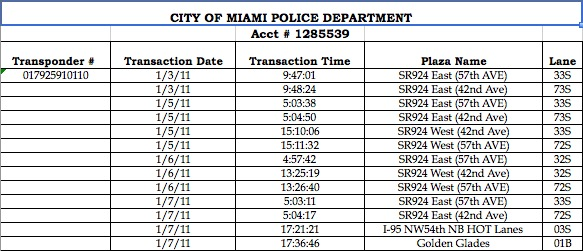
\includegraphics{images/SunSentinalShapeOfData.jpg}
    \end{figure}

When John Maines discovered that every gate in the SunPass network was
synchronized to the National Atomic Clock in Washington, D.C., he knew
they had accurate, calibrated time stamps. Getting the locations was harder
since they were recorded in the data as plaza names, with no lookup for
latitudes and longitudes, nor any mention of the length of road between one gate and the next. It took Kestin and Maines shoe leather, (or at least
tire rubber) and a few trials and errors, to produce those missing pieces of
the data.

Kestin and Maines' first idea for a tool to measure the distances between
gates was the odometer in their cars. They would simply drive the roads
and mark down the numbers as they passed under each gate. But when they
tested the process, they found out that Kestin's Lexus and Maines' Mini
Cooper registered slightly different distances, even over trips as short as 1.6
miles. Worn tires, variation between tire brands, and the general inconsistencies
between cars introduced too much uncertainty.

Their next move was to convince Garmin, a technology company that
designs, manufactures, and markets GPS navigation equipment, to loan
them an Echo200 GPS unit—a \$130 tool that would give them accurate,
reproducible locations and distances. Over the next weeks Kestin and
Maines drove almost every stretch of tollway in Florida. In many cases, they
had to drive each roadway in opposite directions to cater for the variations
in on and off ramps. Through it all, the Garmin returned readings accurate
and consistent to within 1/100 of a mile. (John Maines says that when he ran
spot-checks with Google Maps' driving routes tool they returned distances
consistent with what they'd measured—at least precise enough to calculate
broken speed limits. But they didn't know Google would be accurate until
they'd driven the routes themselves.)

Finally, all the raw data was in place. John Maines' next task was to write the
algorithm in Microsoft Access to show all the trips that broke speed limits.
``When you're doing calculations on tens of thousands of numbers and you
get a formula wrong, everything is going to be wrong. So if you screw up
it could be the end of your career,'' he says. ``The first time I did it, it took
me a few weeks. It would throw out all kinds of errors.'' Meanwhile, Sally
Kestin was reporting out the rest of the story, talking to people who'd been
involved in accidents with police, and asking why, when those accidents
happened, the police escaped heavy punishments.

Nonetheless, the foundation of the story rested on processing the data,
using methods that were new to Maines. ``If I had a chance to go back in
time,'' says Maines, ``I would have told myself how to do this. But I was very
proud to have been able to produce it, and in the end [the results were] very
good, very accurate.''

Kestin and Maines' reporting work seemed to show that between October
2010 and November 2011 Florida police drove their cars more than 6,000
times, not just above the speed limit, but in excess of 90 m.p.h. According to
Kestin and Maines' process, the data held hard evidence of what Floridians
had suspected and complained about: The state's police forces were ignoring
their officers' disregard for the law and, despite deaths and injuries, they
had allowed a culture of reckless driving to grow in their departments.

Despite Kestin and Maines' methodical approach, their editors still pushed
them to prove their process was sound, ideally by consulting someone who'd
done it before. John Maines was assigned to find someone. ``Sally knew of a
traffic engineer, so I called him and he said, 'I can't really talk to you about
it, because I have cases like that in front of the state attorney's office.' '' It
turned out that the engineer had taken the dash-cam video from highway
patrol trooper Donna Watts, who was chasing Lopez, and recorded the
time at which the chased car went under each overpass. That process was
close enough to theirs to give them some confidence. Kestin says her traffic
engineer source calculated Fausto Lopez' speed using the SunPass records
too—the same way they had.

``We took all of our findings to each department we were going to include in
the story,'' says Kestin. ``We took it to them well in advance of publication to
give them a chance to vet it, to make sure that we had not overlooked anything,
to make sure our methodology was rock solid. We said, 'Look, this is
what we got. You tell us—is this what it appears to be?' All of them opened
internal affairs investigations at that point, before we even went to press.''

\subsection{Publication}
Knowing that they had gotten the story and that it was right, Kestin and
Maines were left with the decisions about what to include and the best way
of communicating the facts. Ultimately, they opted to only publish transponder
records for the police who had been driving above 90 m.p.h. on
three or more occasions—more than 25 m.p.h. over the Florida speed limit.

They also needed to choose whether to de-anonymize the data, which would
raise questions of privacy and surveillance. Pragmatism contributed to their
decision not to: ``We could have made public records requests with all 16
police agencies and asked for a list of all their transponders and who they're
assigned to,'' says Kestin, ``but we knew that they wouldn't want to give that
over. Even though this is the great open records state, we figured that could
take another month or two months and it would be a fight.'' But above all
else, Kestin was more interested in showing the police culture rather than
naming individuals. ``I would have hated to name somebody and blasted
their name, their excessive speeds, all over the paper and then have the guy
be cleared two months later. I think we handled it exactly right. I think the
power of this was that never before had these police departments been confronted
with the sheer proof of how widespread this problem was, and how
dangerous it was.''

Fausto Lopez was the exception. In October of 2011, when the video of him
speeding broke, newspapers and TV stations across the United States had
already broadcast his name. Extreme case or not, his was the recognized
face of reckless driving.

    \begin{figure}
    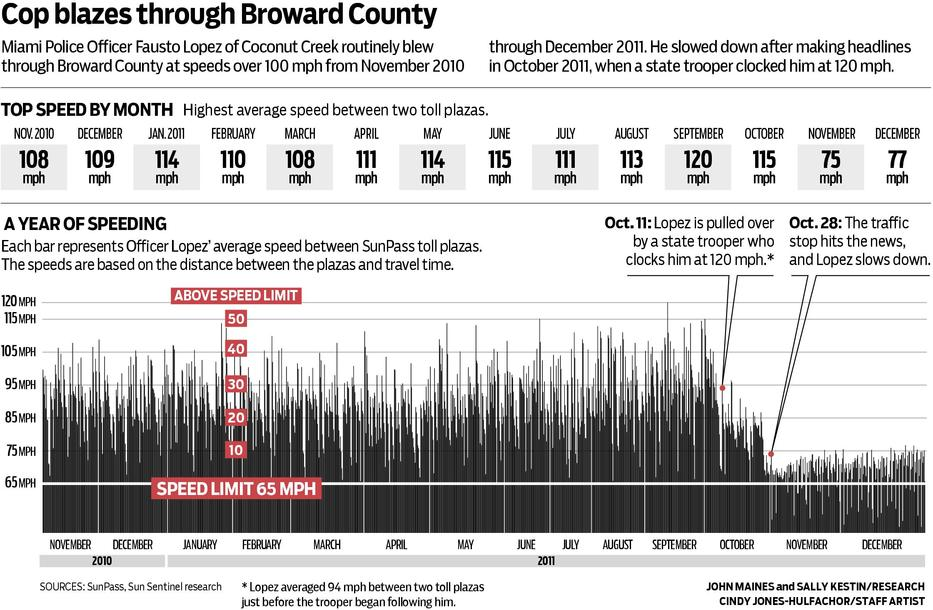
\includegraphics{images/SunSentinalCopsBlaze.jpg}
    \caption{The Sun Sentinel's Graphic.}
    \end{figure}

With such a data-heavy project, there was an obvious opportunity to use
visualization in storytelling. ``I originally did the graph in Excel,'' says Maines.
``My first thought was, 'Let me show his average speed for a month,' and that
looked okay, then 'Let me show his average speed for a week,' that looks
even better, then I said 'Let me show his average speed every single time he
traveled the roads.' That was the origin of that graph with all the hairlines,
and I took it back to the graphics reporter and she put it all together. Everybody
loved that one.''

The Sun Sentinel went on to win the 2013 Pulitzer Prize for public service
reporting. The jury praised ``its well documented investigation of off-duty
police officers who recklessly speed and endanger the lives of citizens, leading
to disciplinary action and other steps to curtail a deadly hazard.'' In
the months after the Sun Sentinel published the story, nine Florida police
departments took disciplinary action against their officers who were routinely
speeding. The vast bulk of penalized officers—numbering 130—came from the Florida Highway Patrol, Miami-Dade Police, and Miami Police.
SunPass records showed that the rate of speeding police dropped by 84 percent
after the Sun Sentinel's first investigation. As Kestin and Maines wrote
in their follow-up story, ``The trend is dramatic and definite: South Florida
cops have slowed down big time.''

\section{Distinctive and Notable}
\begin{itemize}
\item \textbf{Investigative work quantified what was previously a perception.}

Before the Sun Sentinel did its investigation, the case against Florida's
police was anecdotal and unsystematic. By accessing accurate sensor
data and interpreting it correctly, the journalists produced clear, specific
recordings of events occurring in the physical world that could
be objectively compared to legal standards.
\item \textbf{Data was a particularly suitable reporting tool for this story;
confirming a widespread practice.}

A key point that Kestin and Maines succeeded in making was that
speeding was widespread. While journalism has historically used
individual examples to illustrate a problem, often with accuracy and
great effect, the rise of data and accompanying visualizations have
helped journalists better describe widespread phenomena in a memorable
and resonant way.
\item \textbf{A reader sparked the idea for the reporting technique.}

Kestin's relationship and interactions with a reader were crucial to the
reporters' development of their innovative reporting process. It was
a concerned and motivated community member who suggested that
SunPass recorded car movements and might be a viable data source.
\item \textbf{The data processing was done in Excel and Access.}

At the 2014 NICAR conference (the premier data journalism meeting),
the schedule only mentions Access three times, and two of
those mentions are pejorative. Although R and Python are the chosen
tools of many new journalists working with data, in this highly
successful example John Maines used Microsoft Access as his data
processing workhorse.
\item \textbf{The first sensing and verification plans did not work.}

Kestin and Maine originally tried to use a radar speed gun to collect
data before concluding that it wouldn't work. Likewise, their first idea
for measuring the distances between tollgates was to drive the roads
and take odometer readings. In both cases, they did not begin with
the expertise to know the techniques wouldn't work. However, when
their research revealed a problem, they changed their approach.
\item \textbf{The availability of the data relied on SunPass being a
government-owned company.}

The highways and toll-collecting infrastructure in Florida are publicly
owned and operated. That is not the case for all civic infrastructure. In
the words of one influential study into public and private partnerships,
``Governments worldwide have sought to increase the involvement
of the private sector in the delivery of public services.''^{\href{#endnotes-sun-sentinel}{2}} There
are privately run toll roads in states including Indiana, California,
Texas, and Illinois in the United States. Overseas private toll roads
exist in the United Kingdom, Australia, and Spain. It is not clear that
Freedom of Information Act requests would succeed if they were filed
asking for information from tollgates on those roads.
\item \textbf{The data contained errors—which were valid.}

A standard phase in journalists' data synthesis is a ``cleaning'' one.
For data that has been produced by manual, human processes, this
often includes merging alternate notations of the same concept; misspellings
of names, abbreviations, and different labels for the same
object. John Maines, when describing the SunPass data, said it was
``clean,'' meaning it was consistently formed and valid. Therefore, the
data passed through his formulas without breaking. However, some
of the data recorded in the original SunPass files, while valid, produced
results which, when given an eyeball review, were implausible:
speeds of 6,000 m.p.h., for example. While automated error checks
could certainly be written to replicate Maine's human assessment in
the case of a calculated speed 100 times the limit, this is a different
class of wrongness, which may not be as easily detected as the kind of
errors produced by data from manual processes.
\item \textbf{Two people, three months.}

The vast bulk of the work for this Pulitzer Prize-winning story was done
by only two people—Sally Kestin and John Maines—although editors
provided guidance and, in the later stages, editorial assistants, graphics,
and video staff contributed. As Kestin says, ``This project, from
start to finish, only took us three months. In the world of investigative
journalism, that's not a long time. So it's possible to do really high
impact stories without having the big publications' luxury of spending
a year or two and really make a difference in your community.''

\section{Lessons for the Industry}
\item \textbf{Acquire a granular understanding of the sensing mechanism.}

Kestin and Maines made their story bulletproof by, among other
things, gaining a fundamental understanding of exactly how the tollgate
sensing worked. They found out how the tollgate clocks were
synchronized. They investigated exactly where, relative to the tollgate
overhead beams, the RFID tags on cars were detected. Beyond
the mechanics, they understood the administrative processes behind
the data collection, all of which increased their confidence in making
sound conclusions.
\item \textbf{Surround the data with human context.}

Although data provided the conclusive evidence of a widespread
problem, the reporters added touching and powerful stories of individual
people who'd been killed by police driving speeding cars.
\item \textbf{Verify your process with authorities.}

Despite the Sun Sentinel's internal checks and balances, review by editors,
and cross-checking with sources, Kestin and Maines still showed
their data and their process to the police departments featured in
the story.
\end{itemize}

\section{WNYC – Cicada Tracker}
Good radio stations, perhaps more than any other traditional form of media,
thrive on becoming attuned to their communities. Radio hosts like to say
that talkback radio relied on user-generated content long before online
comment threads and photo uploads became de rigueur in the early 2000s.
It's exactly this culture of participation that inspired the WNYC ``Cicada
Tracker'' project from the outset.

It's not immediately obvious that listeners would turn to a radio station to
learn about electronic prototyping, nor that RadioShack would play a part
in predicting a once-every-seventeen-year event in an insect lifecycle. Since
WNYC's data editor, John Keefe, attended one of Make: magazine's Maker
Faire events and took up a hobby of tinkering with electronics, he was looking
for a way to combine WNYC's participation culture with the emergent
maker movement. When he launched the ``Cicada Tracker'' project, perhaps
he might have predicted that folk imbued with New York's entrepreneurial
spirit would also find a way to make the project their own.

In the early phase, when Keefe and his team were casting about for ideas,
their rough concept involved distributing some kind of custom electronic
sensor around a neighborhood, recording some data, and having it sent
back to WNYC. And although they knew their community was interested
in electronics they didn't have a hook to pull people in.

In the winter months of early 2013, a little story lead found its way to the
WNYC newsroom. Every seventeen years on the northeastern seaboard of
the United States, when winter turns to spring and the temperature starts
to rise, the local variety of cicadas (called magicicada) crawl out of the little
holes where they've been hibernating. Unlike most cicada genus, all magicicadas
develop in synchronization, reaching adulthood in the same year.

Through the summer after they've emerged and dried out their wings, the
males' distinctive buzz calls out for mating. For residents near cicada breeding
grounds (rarely the inner city) the cicada months can mean weeks of a
constant background drone.

A good predictor of the cicadas' arrival, Keefe read, was soil temperature.
When magicadas hit their adult year they emerge when dirt eight inches
below ground reaches 64 degrees Fahrenheit. And that is the kind of natural
phenomena that's fairly easy to sense electronically. Many popular starterelectronics
kits include tutorials and parts necessary to build an electronic
temperature sensor in just a couple of hours. The sensors could be placed
in the communities' backyards, producing data to predict when the cicadas
would come out. WNYC would need to add a few customizations, but all
the sensors could be made with easily accessible parts.

The ideal public face broadcast for the project was NPR's hugely popular
science show, Radiolab. In addition to the program's loyal, enthusiastic
community, it had a grant from the National Science Foundation to deliver
informal science education.

The WNYC data news team initially planned to build up to a dozen sensor
nodes and have the data sent back over wireless connections. They wanted
to keep the process simple—easy enough for an amateur to replicate—so
during a hack day, they made a parts-run to RadioShack and spent about
\$200 on an Arduino electronics prototyping kit and a set of accessories.
They then prototyped the wireless version of the sensor, placing a thermistor
at the end of a short length of wooden dowel with wires running back
to a little microchip. They wrapped a plastic baggie around the end of the
dowel that held the temperature sensor to protect it from moisture when
it was stuck eight inches into the ground—or in this case, a nearby potted
plant. At the hack day, the temperature readout came up on a web page.
Later, the team opted for a manual data collection method, using nine LEDs
for the temperature readout, which was far less fussy than trying to set up a
wireless or cellular link.

Altogether, the sensor design that WNYC published online required parts
costing about \$80 and could be assembled in 29 steps, each illustrated with
a picture and a short piece of text. Consequently, people in the WNYC
community actually spent the money, invested the time to build the sensor,
and started to send in their temperature readings. Radiolab presenters
Jad Abumrad and Robert Krulwich talked about the project on air and
promoted hack days for listeners to learn how to build their own sensors.
The team wrote stories online and recorded segments with a professor of
evolutionary biology at the University of Connecticut, Chris Simon, who'd
be collecting the data for her research.

And then, the community went from following the instructions to rewriting
the playbook. In a couple of rooms above 14th street in New York, not
far west of Union Square, there's a small maker-space set up by a group
called Hack Manhattan. An indulgent landlord rents the space to them at a
heavy discount, lets them fill it with a mess of half-used mechanical parts,
electronic works-in-progress, a home-brew beer setup, multiple 3D printers,
and a few benches where members come in to work on whatever kind
of craft project piques their interest. Guan Yuan was one such member,
who worked on occasional electronics projects between studying business
at NYU, tweeting wittily and prolifically, while blogging occasionally.

He'd also been to a class run by NYC Resister, a hacker collective based
in Brooklyn with the slogan ``We learn, share, and make things.'' They'd
started to teach him how to take an Arduino prototype and pare it back to
its essential components; making it cheaper to build, more efficient to run,
and devoid of any wasted resources.

The Arduino electronics platform was released in 2005 by an Italian interaction
design professor named Massimo Banzi who wanted a tool for his
students to learn electronic hardware development. At the center of an
Arduino kit is a cheap microprocessor that runs code recognizable in the
c++ family. The microprocessor is attached to a circuit that connects power,
a numerous and varied set of communication pins, and a USB port that
can deliver data to a Mac or PC computer for programming. A store-sold
kit normally includes a bread-board, which developers can use to wire-in
sensors, data loggers, wireless communications, lights, or any number of
different interfaces they choose—all without ever powering up a soldering
iron. Arduino's open source hardware and software affords accessibility,
low price, and lots of flexibility. These attributes have made it wildly successful.
By April of 2013 customers had bought more than 700,000 official
boards and the founders estimate that for every official board there is a
(legal) clone running.

However, Arduino's design and intent come with tradeoffs. If a developer is
only planning to use the platform for a single application, he or she won't
need the easy re-programmability that comes with plug-and-play computer
connections. Likewise, there will probably be far too many communication
pins and the breadboard is surplus to requirements.

Through Twitter, Guan Yang heard about WNYC's cicada project, but could
easily see ways that the original electronics design could be re-worked
to bring the hardware cost way down. Thus, he intended to sell specialized
cicada tracker kits at a Hack Manhattan's maker day. Part of his plan
improved the design and leveraged the remarkable economics of the international
electronics industry.

The key to reducing cost in his new version was moving away from the
Arduino-branded and bundled parts, and buying only the minimum
amount of components from a cheaper distributor—instead of using the
full starter Arduino kit RadioShack sells at a considerable markup over the
parts' cost. Yang's kit avoided the use of a breadboard, replacing the flexible circuit board with a printed circuit board (PCB) and swapping out the overpowered
brain of WNYC's design, an ATmega328P microprocessor, for its
slightly cheaper variant, the ATmega168P.

He designed the new circuit board using KiCad, a program that's widely
used by the open source hardware community, and sent his design files
(known as gerbers) to Smart Prototyping, one of the cheap Chinese board
houses that accepts orders for short production runs of electronic parts.
The factories in Shenzhen, China, printed the boards, and a couple of weeks
later—for a total cash cost of \$87.86 (of which \$22.80 was shipping)—50
circuit boards arrived in New York via mail; the price per board was just
\$1.75 and the microcontroller cost about \$2.40. So just by replacing the
``Cicada Tracker's'' Arduino core with his custom PCB and the microprocessor,
Yang reduced a \$30 parts cost to \$4.15. The other necessary components—
the thermistor, LEDs, batteries, and wiring—cost only a few more
dollars meaning Hack Manhattan could sell a whole kit, complete with
LEDs and a temperature sensor for \$20, which still included a good profit.^{\href{#endnotes-wnyc}{1}}

Yang says he put a total of 11 hours into the project. While hack day attendees
did buy some of the kits with a printed circuit board (PCB), a more popular option was an
alternate kit the Hack Manhattan members put together (also for \$20, but
with a lower profit margin), which had a breadboard instead of the PCB,
giving buyers the ability to reuse more of the parts for other projects.

From WNYC's first prototype to Yang's streamlined model, the component
cost of the cicada tracker had dropped 90 percent. WNYC designed
its own cheaper breadboard version based on Yang's design and gave them
away at public events to listeners and institutions from along the northern
East Coast.

As the cicada season progressed, from anticipation, through arrival, into a
noisy summer, the WNYC data team opened the doors to reports of cicada
sounds and sightings. John Keefe says that by the end of the project, contributors
had sent in more than 1,750 temperature readings from 800 different
locations. When the cicadas started to emerge, contributors filed another
4,300 reports recording where and when they'd seen new cicadas, aside
from any temperature data. Those are big participation numbers for any
kind of journalism project, but they're even more impressive considering
the fact that they demanded people first learn about electronics, assemble
a kit, stick a temperature sensor into the soil, read the temperature from a
pattern of LEDs, and submit the reading using an online tool. As Keefe says,
``From an engagement standpoint in journalism, that's kind of amazing.''

\section{Distinctive and Notable}
\begin{itemize}
\item \textbf{An archetype for a particular model of using sensors
in journalism.}

The WNYC ``Cicada Tracker'' was probably the first time a major
media organization had so explicitly combined the activity of electronics
and sensor prototyping into a journalism project. They placed
sensing at the forefront of the participatory experience. This flavor of
media sensor use was distinctive, clearly innovative, and pointed at a
new realm of worthwhile experimentation and approaches.
\item \textbf{Participation and radio go together like sensors and Arduino.}

WNYC's efforts to train its community to participate in data projects
had a head start. Radio, as a medium, needs a variety of voices to be
sonically interesting, and to reflect the identities in a station's listenership.
Talkback is one of the main ways radio stations achieve that (it's
also relatively cheap). An early WNYC data project asked New York
listeners to send in their neighborhood's prices for milk and a six
pack of beer. Through running projects like these the online teams of
WNYC have developed an instinct for how to evolve their participatory
culture from radio to digital.
\item \textbf{This shows an evolution in digital participation.}

From mainstream media audiences, we are used to seeing participation
in the following forms:^{\href{#endnotes-wnyc}{2}} (Listed here in rough, arguable, order of
user effort) 1) Clicking ``like'' or recommendation buttons, 2) distribution
on social media and email, and 3) contributing to comment
threads, call-ins, writing letters or emails, photo and video contributions.

In this case, the WNYC's community engaged by building, and
then redesigning, electronics. Precedents exist, of course: Open
source software and hardware communities flourish online, although
legacy media companies' audience-facing operations rarely interact
with them. Make: magazine is built on, and for, such people—and
puts them under an umbrella with the craft communities who cook,
garden, sew, and knit.

In Sydney, Australia, the ABC 702 local radio station hosts a yearly
``knit-in.'' In the preceding months, its community designs, then builds
(knits) garments and toys. That may not be electronics, but it's still
maker participation. Nonetheless, WNYC was the first mainstream
media organization we know of to successfully encourage a non-trivial
number of people to build electronics and contribute sensed data.

\item \textbf{In this case, the accuracy of the data wasn't actually central to
the project.}
Even beyond the question of whether WNYC's community temperature
observations were accurate, one might ask whether the optimum
strategy for predicting the cicadas' arrival was to deploy home-built
sensors; especially while having minimal control over their geographic
distribution, or the consistency of their operation once in the
field. John Keefe has acknowledged that more accurate predictions
could certainly be made based on official air temperature readings
and soil-type models.

However, that question mistakes the benefits of the ``Cicada Tracker''
project, whose goals included informal science education. Keefe
argues that many of the people who built the sensors were using
Arduino for the first time, and were thereby exposed to electronics
prototyping—a growing movement. They learned about the relationship
between cicada life cycles and their natural surrounds. They also
enjoyed the benefit of participating in a communal activity. The data
may or may not have been accurate or useful, but it is inadequate to
emphasize that goal to the exclusion of the project's other outcomes.

\item \textbf{The conditions were perfect for a price drop from \$200 to
about \$12.}
WNYC spent \$200 on a kit of parts, many of which were superfluous,
to build its first version of the cicada tracker. A few weeks later, Guan
Yang acquired the parts for about \$12. But consider the confluence
of events and ecosystems that reduced the cost so much: The radio
station operates in New York, a city dense with creative technologists.

The project caught the interest of a Twitter community who
discussed and distributed the idea. A person who was on Twitter and
was interested in electronics had also attended a course focused on
just this problem space. The evolution of the Arduino platform made
the project conceivable. Arduino itself is an artifact of and an accelerant
for the cheap electronics ecosystem that makes it possible to have
50 totally new and customized circuit boards delivered from a factory
in China to a door in Manhattan in less than two weeks for less than
\$100. The implications of this are outlined below.
\end{itemize}

\section{Lessons for the Industry}
\begin{itemize}
\item \textbf{Motivated and engaged people will contribute a lot of effort.}

Audiences contribute no reaction at all to plenty of media output,
as evidenced by the vast fields of published news stories and blog
posts languishing with unpopulated comment spaces and zero ``likes.''

In this case, however, people in WNYC's community bought parts,
assembled them through 29 steps, wrote code, took sensor readings,
and manually contributed them via an online form. One person (operating
within his own community who contributed help), went even
further by refining WNYC's designs and producing a newly improved
version. This contribution of time, intellect, and work may hint at
untapped potential, especially if a project has avenues for entrepreneurial
and creative community members to get involved.
\item \textbf{Use publicity and ease-of-use techniques to engender
motivation and engagement.}

The ``Cicada Tracker'' project pulled some good moves: Although
the project originated at WNYC's data desk, Radiolab heard about
it, reached out and came on board as its public face. Radiolab's audience
is interested in nature science and the hosts have a strong relationship
with their community. WNYC designer Louise Ma made the
instructions extremely easy to follow, reflecting the project's overall
approach of very clear communication, assuming no prior knowledge
but without condescension. The tone of the project combined
learning and fun. One WNYC event was held at a beer brewery where
attendees could make sensors and meet Radiolab host Jad Abumrad.
\item \textbf{Be open to the community.}

The unanticipated and unasked-for innovation by the Hack Manhattan
members significantly expanded the project's reach.
\item \textbf{Realize the implications of cheapening technology.}

WNYC's ``Cicada Tracker'' project appears to demonstrate the economic
feasibility of journalism projects producing and using customized
electronics. Achieving a parts cost of less than \$20 seems to
open up the potential for media companies to deploy large numbers
of sensors (or have lots of their community build and deploy sensors)
designed to produce data for just one story.

While this was the case for this particular project, there were a number
of distinct factors that were not universal. Guan Yang, who has a
set of electronics design and production skills that are currently rare,
contributed his time at no cost. The ``Cicada Tracker'' also comprised
a basic set of hardware: the low-end thermistor was a very cheap
sensor; it didn't need a screen display, data storage or networking;
and there was no real miniaturization nor need to make an appealing
form-factor. If those factors are not in place, customized hardware
development can get very expensive, very quickly. At a unit price of
\$100, a project requiring just tens of sensor nodes moves beyond the
budgets available to most newsrooms, and above what many individual
audience members are willing to spend. 

Nonetheless, if the
field continues, the skills of hardware design and build may become
more widely distributed (even into news developer teams), and the
ecosystem may produce hardware components that fulfill more
journalistic needs.
\end{itemize}

\chapter{Planet Money – Planet Money Makes A T-Shirt}
The public radio show Planet Money raised more than half a million dollars
to make a T-shirt. Its Kickstarter campaign attracted 20,159 backers
pledging at least \$25 each for a short-sleeved shirt made out of cotton with
a printed cartoon squirrel holding a martini glass—and to pay for Planet
Money to document the production process ``from seed to store.''
Aside from the T-shirts themselves, the end result was a series of radio
episodes, a Tumblr, and one of the most impressive interactive documentaries
of 2013. The online video unobtrusively incorporated footage shot
from a high-end cinematography drone flying around a Mississippi cotton
farm. Josh Davis was the project's video director, brought in by executive
producer Alex Blumberg.
While the farming chapter, which used the drone photography, is the first
bit of video that appears in the documentary, the crew didn't start planning
it in detail until after shooting the other chapters in Bangladesh and Colombia.
The overall vision for the film had the story split into chapters. It would
start in Mississippi, showing the cotton being harvested, then move through
Indonesia where the cotton was turned into yarn and fabric. Next the story
would split off to Bangladesh where the factory workers made men's version
of the T-shirt, and to Colombia where they made the women's.

Throughout the international shoot, the crew had looked for ways to collect
unconventional shots. Back in the United States, they continued the
trend, strapping GoPro cameras to boxes moving down conveyer belts, and
rigging another to the corner of a shipping container that transported the
shirts by ship, truck, and train. (In fact, one of their unattended traveling
GoPros was ripped from the outside of their container somewhere between
Jacksonville, Fla., and North Carolina.)
In the film's first chapter, Blumberg and Davis wanted to show a crucial
element of the story—the sheer magnitude of the United States' modern
cotton farming industry. The farm near Clarkesdale, Miss., where they
filmed stretched over 4,000 acres of land. The owner, Bowen Flowers, sells
13,000 bales of cotton to the garment industry each season, enough for
9.4 million T-shirts.
The wildly successful Kickstarter campaign meant that the project was fairly
well funded. They had enough money to think big, in Davis' words. ``If there
was ever a time to take a helicopter, this would be it.'' But that was before
Davis hired a freelance director of photography, Eric Helton, who showed
the team a Range Rover commercial featuring footage shot from a drone
flying in the Utah desert and Colorado mountains. According to Davis, that
was the ``oh shit moment'' for him and Blumberg. Mostly, they'd not been
serious about hiring a helicopter, but the quality and style of the advertising
footage made the aerial footage seem feasible and desirable. Indeed, Davis'
only concern was that the video might seem too slick, giving the documentary
a commercial feel.
Davis only considered one company: SkysightRC, who shot the Land Rover
commercial. Two brothers, James and Soren Jensen, run the agency out of
Colorado, mostly shooting commercials and adventure films in the United
States and nature documentaries overseas. After Davis and Helton talked
the job through with the Jensen brothers a couple of times, they decided
they didn't need to ask for any other quotes.

SkysightRC's normal day rate is \$3,500, but the figure moves about depending
on how many days the shoot covers, and the kit the brothers take along.
For the Planet Money job, they used a Cinestar octocopter—an eight-armed
craft a meter across with 14-inch rotors spinning at the end of each arm.
Fully loaded it weighs about 14 pounds. The base kit costs about \$8,000, but
buyers who are looking for better results spend much more on parts like
controllable anti-vibration camera mounts, plenty of batteries, and live
video downlinks. Despite the emergent nature of the field, and the battles
around professional civic drone flying, SkysightRC has been able to buy
insurance for its business.^{\href{#endnotes-planet-money}{1}}
The crew met in Mississippi for the first time on the night of October 6,
2013, with Bowen Flowers' farm due to start harvesting cotton over the next
two days. The four key shots it wanted to use would take advantage of having
a small, incredibly maneuverable craft that could give viewers an exhilarating
sense of the vast scale of the cotton fields. Drone enthusiasts have
learned to recognize the craft's distinctive moves; transitions between tight
shots and aerial angles, swoops around large objects, and shots tracking
moving subjects over long distances.
The two brothers from SkysightRC work as a team. On this shoot James
took responsibility for flying the craft while Soren watched an LCD screen
showing live video feed from the onboard Sony FS100 video camera; he
controlled the camera angle remotely.
In the pink early-morning light the next day, they sent the drone climbing
just above the cotton flowers right up to a height beyond the reach of
any camera boom. In another shot they flew the drone very closely over
the massive crop picker; and in another it's skimming along the top of
the plants.

On the shoot, James and Soren work standing next to each other. In Davis'
words, ``They go into the zone. One's kind of hippy, the other is kind of serious.
They're calling out the shots and the moves to each other.'' The final shot
they needed from the drone's capabilities used it as a static camera mount
pointing down from high above as the harvesters crossed underneath.
In the final two-minute and thirty-two-second video chapter, the editors
used about 40 seconds from the drone footage, of which 15 seconds is the
establishing shot and 15 seconds is a closing landscape shot. The three
remaining short clips are action shots of the cotton and the mechanical
pickers doing their work. The drone-shot footage doesn't call attention to
itself; it's entirely integrated—only enthusiasts can notice the innovative
technique used by the crew.
When Planet Money's interactive documentary went online it spread around
social media and has attracted 600,000 visitors who stayed on the page for
an average of 32 minutes. In the first few months of 2014, the project picked
up second place in the National Press Photographers Association award for
Best Multimedia Package, a Photography of the Year award from the Missouri
School of Journalism, and a Society of News Design award.
Distinctive and Notable
\begin{itemize}
\item The drone was not foregrounded.
While audience members familiar with drone footage found it easy to
identify in Planet Money's online documentary, general viewers might
be unaware of the production team's innovative approach. The team's
Tumblr, where it published production updates and featured a couple
of photos from the Mississippi shoot day, doesn't draw attention to
the drone itself. By contrast, when some other journalistic entities—
like the BBC, CNN, and a few non-mainstream media pilots—have
made use of drones in the past producers have pushed the technique
into the foreground, sparking plenty of attention on social media and
commentary on other media sites but perhaps overshadowing the
original story.
\item The team sacrificed a GoPro.
While the Tow Center's main motivation for writing about this case
was to study its drone use, the production team's use of GoPro cameras
was another expression of the same technological trends that
have made drones intriguing as journalistic tools. Put simply, one can
now pay far less to buy technology that can do far more. It was therefore
economically feasible for the videographers to put cameras capable
of capturing excellent HD video in places where camera operators
couldn't reach—and where the cameras could easily get damaged or
lost (probably even stolen).
\item All the conditions were in place for innovation.
This was a production with a healthy budget. It had far more money
than most single-story projects originating from public radio/online.
Although it didn't have a TV-sized budget, neither was it entrenched
in television's conventional ways of shooting aerial video—from a
helicopter. Unlike video journalism teams who work on ongoing productions,
sometimes falling into habits, the personnel for this project
were pulled together anew. Each had recent experience circulating
through different professional fields, from agency photojournalism,
to magazines, to commercials. Their brief was to be adventurous; they
had the resources to match the ambition and the team was fresh.
\item The Jensen brothers tolerate a lot of legal risk in their business.
Through the last year, the Tow Center has conversed with a number
of media companies that have ambitions to use drones inside the
United States for journalism. Our standard interpretation of the legal
landscape is that journalistic use of drones is highly risky. Indeed,
the FAA claims responsibility for regulating civic drone use in the
United States, asserting that journalistic use would be illegal (see the
legal and ethical section of this report for more detailed discussion
on that topic). However, the Jensens have built a business that draws
some of its revenue from drone use inside the United States. They
have also been able to buy insurance for domestic use. It should be
noted, however, that they are aware of the safety risks, and work to
minimize them.
Lessons for the Industry
\item Hire the pros… perhaps.
Josh Davis, the video director for this project, was adamant that the
only way to shoot drone video was to get specialists involved. He says
that after witnessing SkysightRC's sophistication, level of control, and
extensive practice he knows without a doubt that producers should
hire professionals. However, as the Tow Center's recent report on the
state of online video suggests, the field is rapidly changing.^{\href{#endnotes-planet-money}{2}} It may be
that Davis' recommendation holds true when producers are aiming to
make Planet Money's variety of very high-production value video, but
alternative approaches may be valid for applications like breaking
news and community contributions.
\item Let the story dictate the use of drones.
In the planning process for this production, the team began by establishing
the story it wanted to tell. Once Davis and Blumberg understood
how crucial it was to convey the incredible expansiveness of
the Mississippi cotton farm, they then started to think about how to
render that coverage. As a result, the footage serves the story.
\end{itemize}

\section{Washington Post – ShotSpotter Tracks Gunshots in D.C.}
The Washington Post's coverage of the ShotSpotter system was actually a
byproduct of a different story David Fallis was reporting. Guns have been
a major topic around Washington, D.C., for many years. Over a ten-year
period, the police departments in Washington and nearby Virginia recovered
nearly 50,000 of them. The region has a metro population of about
six million people. While reporting that story during the spring of 2013,
David Fallis talked to a source who told him about a presentation at a police
conference that drew on data from a system called ShotSpotter, an array of
audio sensors installed around the city.
In Washington, D.C., ShotSpotter's microphones sit on rooftops and near
surveillance cameras, monitoring areas for noises that sound like gunfire.
When a microphone hears a likely match, it activates a recorder that saves
the sounds and sends the data back to the D.C. Metropolitan Police Department's
centralized control system. As data from other ShotSpotter microphones
comes in, it gets compared and triangulated to produce a location
alert—all within a few seconds. Washington police say the system means
they don't have to rely on neighbors calling 911 to find out about gunshots
and get their patrols out to the right places to start investigations. Fallis
thought the system itself was underreported, and that an aggregation of
those gunshot reports might have its own story to tell.

Fallis couldn't get the ShotSpotter story to fit into his original piece about
gun confiscations, but over the summer and into autumn he began working
on the story with two other Post reporters, Dan Keating and Ted Mellnick,
with assistance from Andras Petho, an investigative reporter from
Hungary who was interning at the Post. In November The Washington Post
published their story as a special investigation on the front page of the
Sunday paper, matched online with extensive videos, data visualizations,
audio, and graphics.
Early on, Fallis got in touch with the D.C. police to obtain the ShotSpotter
data. Initially they declined to release it unless Fallis filed a formal Freedom
of Information Act request. The application went in during April, with Fallis'
main gun confiscations story due to run in May. The D.C. police department
conceded that the data was public record and said it was prepared
to release it—however, the intent didn't translate into action. The problem,
according to Fallis, was not one of the police department's will, it was an
issue of mechanics. The police department proposed printing out individual
gunshot reports on separate pages, a process that would produce reams
of paper. In Fallis' words, the paper parcels would have been ``outrageously
large, especially in today's digital world.'' Petho called around to other
American cities' police departments that had installed ShotSpotter systems
and found that they were all able to export data as Excel spreadsheets with
the touch of a button.
The reporters also started to establish relationships with people who worked
at the ShotSpotter company. In the end, they asked the ShotSpotter staff to
help the D.C. Metropolitan Police Department get them the data.
David Fallis' interpretation of the police department's apparent lack of technical
expertise with its own system hinges on the fact that the reporters'
motivations for wanting the data were so different from the department's.
The police use the system in real time; a gunshot triggers an alert in the
system, which tells officers where the gunshot came from, down to an area
five-feet in diameter. They send a patrol to the spot to start their work and,
in many cases, that's where their use of ShotSpotter ends. Individual reports
might be used in court, but for D.C. police, ShotSpotter is a daily operational
tool.
Fallis was much more interested in analyzing the data for patterns over
the years and spatial clusters around particular neighborhoods to show
frequent gun use. The only other individual reports that Fallis particularly
cared about were those that could be compared to incidents that the Post
had written about—and that was mainly so he could try to verify the system's
accuracy.
However, in the case of ShotSpotter, the very concept of accuracy is
marred by seemingly unavoidable technical nuances. According to the
company, fireworks are the greatest source of false positive reports since
they produce relatively short, explosive sounds just like gunshots—further
complicating data errors around holidays and festivals. ShotSpotter representatives
say that in plenty of the cities where the company has installed
systems, gun owners also shoot off celebratory gunfire. The Post reported
those shots account for around a third of the gunshots ShotSpotter registers
in Washington, D.C.
Changes to the system over the years further confounded comparisons
between data sets. The FBI was the first to fund ShotSpotter in Washington,
D.C., responding to the city's very high homicide rate. The agency first
put the microphones out on rooftops in a few areas. Over time, it passed
responsibility for the system over to the Metropolitan Police Department
as part of the department's expansion during the administration of Police
Chief Charles Ramsey. In 2007 the police department signed a new contract
with ShotSpotter, whose acoustic experts came in and adjusted their sensors'
placements, and installed different kinds of microphones in new locations
as new bits of funding became available for the initiative.
Comparisons between places were also complex. The police department
only installed microphones where it suspected there were gun problems and
moved them as the situation changed on the ground. There was no record
available of exactly when each alteration was made or what was moved each
time, which prohibited the reporters from making local comparisons, such
as gunshots in Prince George County to those in the District of Columbia.
ShotSpotter wouldn't give Fallis information about what its systems found
in other cities. The company also refused to release a complete list of cities
that had installed the system.
The reporters also considered whether or not there was a privacy and surveillance
angle to their story. Each node of the ShotSpotter system is a
combination of a microphone and a customized computer that monitors
the microphone and turns on the recording when it recognizes a sound
matching a gunshot signature. ShotSpotter says that the wave files the system
sends back are only a few seconds long. In some cities, ShotSpotter
has been integrated with security camera systems, so that when it identifies
a gunshot, cameras in the vicinity rotate to point at the calculated origin.
However, this has yet to be implemented in Washington, D.C. Ultimately,
the reporters concluded that there was not a significant privacy angle to
their story.
The data that the Metropolitan Police Department released came in an
Excel file, with a relatively simple structure: Just over 39,000 rows; one for
each shot, containing the police administrative area, an ID number, a timestamp
plus longitude and longitude figures to three decimal places.

The Washington Post published its story in early November of 2013. Online
the story ran at about 3,500 words, featured highly produced video, photos,
and three interactives. The journalists presented their coverage with two
aims; first to explain what ShotSpotter was and how it shaped Washington
police operations, and second to interpret the data and give readers the
chance to explore it and find their own narratives.
The explainer section walked readers through the evolution of the technology,
from a Californian inventor's passion in the early 1990s to its current
state and presence in 65 American cities. The Post reported that D.C.'s system
had cost about \$5.5 million over the eight years since it was installed in
2005. It described the microphones, their placement, and the software that
interprets the sound waves, while giving a couple of examples of criminal
cases where ShotSpotter became central to police investigation.
As an illustration of the system's technical complexity, the Post's designers
built a tiny game allowing readers to test their ability to identify the difference
between gunshots and fireworks, using examples from the ShotSpotter
database.
Figure 1: By Bonnie Berkowitz, Emily Chow, Dan Keating, James Smallwood, The Washington Post
The Post's interpretation of the data started with the spectacular headline
figure—``39,000 Shooting Incidents in the District''—and continued with
other statistics in the written story, infographics, and interactives. The
reporters noted that SpotShotter more than double the number of gunfire

incidents than there were official gun-crime reports. They wrote that Washington's
detected gunfire had dropped off by 40 percent since 2009, and
isolated a few hot spots with even bigger reductions.
The newspaper also built an interactive, which played a slightly different
role in rendering the data. Its visualization needed to give users the ability
to explore the data to find personally relevant views, while grappling with
the fact that the location data was only precise to three decimal places. In
latitude and longitude numbers, three decimal places is only enough to
denote a location within a 100-meter area.^{\href{#endnotes-wapo}{1}} The police had truncated the
data to protect the privacy of Washington residents in the ShotSpotter
coverage areas.
The graphic designers' solution was to produce a kind of gridded heat
map. It represented the data's geography, showed the intensity of the gunfire
in various areas, but avoided depicting it with more precision that the
data warranted.
Figure 2: The Washington Post's map, zoomed out.

Figure 3: The Washington Post's map, zoomed in.
Even though this was a data-backed story, in line with the Post's normal protocol,
Fallis supported the choice not to publish the underlying files, despite
attracting some criticism. ``It's meaningless to most people; our job is to
make sense out of stuff. It's not like a nursing home inspection database
where somebody can type in grandma's nursing home and the reports are
up there. We've done that kind of stuff. This one, frankly, I didn't think was
a very sexy click-magnet apart from the context we put it in.''
Carlton Purvis, a D.C.-based journalist with an acute interest in security
and surveillance, had a different view. He filed his own FOIA for the
data, and posted it, along with a simple interactive map, on the website
PublicIntelligence.net.
When users zoomed in on the PublicIntelligence map, they saw the data as
dots plotted in a grid. PublicIntelligence's overly precise mapping of data
evoked some mistrust. One commenter wrote, ``This graph is bullshit. Zoom
in, all the data is evenly spaced. Complete bullshit. Next.'', which attracted
the response: ``The points are evenly spaced because LAT/LONG data is
truncated to three decimals (for obvious reasons). This results in a ~100yd.
grid. Please apply a tiny amount of intellect before calling bullshit. Next.''

Figure 4: Carlton Purvis' interactive on Public Intelligence.net
Both before and after The Washington Post's story, newspapers from Atlantic
City, N.J.; Oakland, Calif.; and many other cities have published stories
about crimes the ShotSpotter system detects or how their cities fund installations.
Although ShotSpotter keeps its full client list confidential, the company
says it has more than 80 installations in place, of which more than 70
are in the United States. It lists two Brazilian cities as clients, and boasts of
installations in four countries. Still, the story that Fallis and his colleagues
published in The Washington Post appears to be the only ShotSpotter reporting
that had access to the system's data.
Distinctive and Notable
\begin{itemize}
\item Sensor data was used in a way unanticipated by its developers.
The Washington Post's story used the ShotSpotter data in ways that
neither the system's designers nor the police agency intended. As such,
there were delays in exporting the data since the police did not use the
data in aggregate; reporters needed the vendor's help in producing it.
Ultimately, what may have looked like deliberate data obstruction on
the police's part was simply the result of missing skills.

\item The historical alterations of the system limited analysis.
Similar to the point above, The Washington Post had to contend with
the fact that it simply couldn't make broad comparisons over all the
years that the ShotSpotter system had been in place. Again, the police
used and deployed the sensors as a day-to-day operational tool, not
one of analysis. When the department thought a certain neighborhood
needed more or less coverage, it changed the number of microphones
there. When new contracts were signed, the system was reworked.
\item Publically funded data wasn't necessarily easier to obtain.
Installations of ShotSpotter equipment throughout the United States
(and in some other countries) used for police surveillance are funded
out of the public purse. However, this didn't necessarily mean the Post
could get the data as a public records request. For good practice and
to further inform this report, the Tow Center made public records
requests from two other cities that have installed ShotSpotter. Atlantic
City, N.J. police refused the request on the basis that releasing the
data ``could lead to the system being compromised as the location of
[its] sensors is confidential. The exact coverage area is also confidential.''
They told us, ``The data you are requesting could be used to track
the location of the sensors.'' Camden, N.J. police initially said that they
needed to get the permission of the ShotSpotter company itself. The
Tow Center obtained permission, and, for the 13 subsequent weeks at
time of writing, has been corresponding with Camden police representatives
on a weekly basis to no avail.
\item Decisions were made about how much of the data to publish.
The lead journalist on the investigation, David Fallis, opted not to
publish the raw data. In contrast to some data journalists' ``show your
work'' practice, he saw risks in being held responsible for the accuracy
and freshness of the underlying data, reasoning that the originating
police department was a better source. He did help curious people
contact police and form their records requests.
\end{itemize}

Lessons for the Industry
\begin{itemize}
\item Make sure data visualizations relay your findings with clarity,
even when the data has limitations.
Although The Washington Post and Public Intelligence both mapped
the same data, there was a notable contrast between their treatments.
The Washington Post deployed its considerable graphics resources to
produce a highly specific visualization approach, combining a heat
map with a customized grid (that avoided overstating the data's precision)
and mouse-over information panels. Public Intelligence, on
the other hand, mapped the data in Google Map's default format—
point markers. While this represented the data reasonably well when
zoomed out, it was overly precise when zoomed in. Comments on its
site evidence audience confusion.
\item The sensors themselves were newsworthy.
In this case, the investigative and graphics journalists put a huge
amount of effort into explaining the system itself. Those implicit news
values suggest that sensor systems like ShotSpotter are, for a general
audience, novel, opaque, and not generally understood. While journalists
may find it worthwhile to use data from sensors to tell stories,
they may also find readers are interested in new types of sensor systems,
how they're being incorporated into civic life, and their broader
ethical, legal, and social effects.
\end{itemize}

\section{Drones for Journalism: An Overview of the U.S. Industry}
The field of drone journalism in the United States is unlikely to remain
static. Just a year ago, there were very few known examples of journalists
using drones to report local stories and we knew of only a handful of cases
internationally. Recently, though, we've seen a number of journalistic works
incorporating quality video shot inside the United States using high-end
drones. We have more evidence of enterprising photojournalists experimenting
with cheaper camera drones to cover breaking news and color
stories. Beyond these uses by news industry employees, we have also seen
drone footage by hobbyists find its way into mainstream media.
The Federal Aviation Administration, which has regulatory authority over
U.S. airspace, asserts the right to regulate small drones, but its sole prosecution
to date was dismissed by an administrative law judge.^{\href{#endnotes-industry-overview}{1}} The FAA immediately
appealed to the full national safety board. Regardless of the eventual
outcome of the case, additional bodies of law and ethical principles will
affect how journalists use drones. A separate section of this report explores
those issues in detail and describes the regulatory outlook. While the difficult
legal environment has slowed journalists' use of drones, it hasn't
stopped it entirely.

A Typology of Drone Use
Despite the pace of change in drone journalism, rough groupings have
emerged: high-end specialists, enterprising generalists, and ``the crowd.'' It
seems credible to predict that this typology will last.
The case study about NPR's Planet Money and its use of a cinematography
drone, found earlier in this report, represents the high-end style of the field.
To film a portion of a documentary, the team hired SkySightRC, a small
agency that uses tens of thousands of dollars worth of kit and flies as a twoperson
team: a camera operator working in tandem with a pilot. ABC News
used footage by the same company for its coverage of the Colorado floods
in September of 2013. The advertising and movie industries employ similar
companies, both domestically and abroad. Overseas, the BBC and the Australian
Broadcasting Corporation take the same high-end approach—expensive
equipment operated by at least two highly trained people with lots of
attention paid to the safety of the people in areas where they fly. Considering
the contested legality of professional civic drone use, it may be surprising
that at least three insurance companies have been prepared to write policies
covering professional camera-drone flights inside the United States.
To understand generalists' use of drones, a useful source is a survey run by
the National Press Photographers Association in March of 2014.^{\href{#endnotes-industry-overview}{2}} The results
revealed that many newsrooms across the country are experimenting with
small drones for journalism. The precise number is very hard to confirm:
172 survey respondents to the NPPA survey (who did not have to state their names or employers) said their companies had actually used a drone for
newsgathering.^{\href{#endnotes-industry-overview}{3}} Mostly, these were small consumer-grade camera drones
costing hundreds, not thousands, of dollars.
The Stories
The subject matter of drone-shot footage varies. Professional photojournalists
and camera operators have shot the aftermath of natural disasters and
traffic accidents for breaking news. As color pieces, they've filmed spectacular
architecture, crowd events, picturesque weather, and landscapes.
An even larger number of respondents, though, said they wanted to use
drones but were prevented by legal restrictions, safety concerns, and the
expense. Journalists who fell into this group said they would use drones in
the same ways as their bolder peers, noting additional benefits.
A number of respondents said they would employ drones to get around
obstructions; either for reasons of personal safety, police restrictions, or difficult
environments. A few vivid examples:
\begin{itemize}
\item `` Recently we had authorities burn down a house filled with
explosives. A drone would have helped us get images of action
going on at the scene and the fire itself.''
\item `` We did a video about the fifth anniversary of the closure of a
GM plant. It would have been nice to go on an adjoining property
and do a fly by to see the sprawling facility at more than eye
level. Instead, we just drove by the fence and shot video.''
\item `` Drone aircraft could have given us better perspective on a story
we are covering right now: ice jams in a river and the threat of
flooding. We cannot safely get close-ups of the problem with a
news crew. A drone could fly, give us a better angle and safer.''
\item `` Pretty much any story that police calls a crime scene.''
\item `` Major news events where access is limited and roadblocks prevent
us from getting close enough to get the shots needed.''
\end{itemize}

The Economics
Respondents repeatedly cited the lower cost of drones in comparison to
helicopters as a significant benefit. In the words of one respondent: ``For
my helo costs, I could probably have a dozen HD-capable drones in the air.''
Another wrote, ``The cost of using a helicopter or fixed wing aircraft is high,
anywhere from \$400 to \$1,800 per hour. A drone, such as the DJI Phantom,
costs less than \$23 per hour, making aerial news photography cost effective
for daily use.''
Around two thirds of the survey respondents worked outside the TV industry,
meaning they hadn't traditionally been able to pay the helicopter costs
necessary to obtain aerial footage. However, that part of TV's competitive
advantage may be in danger. One respondent wrote, ``Our competitors have
helicopters and are [using them to get footage from news events where
access is limited] every day. Although they are paying an expense my company
won't cover.''
The Risks and Concerns
When it came to the risks and problems associated with drone use, the
main points of interest concerned privacy and safety. With regard to privacy
concerns, NPPA survey respondents' attitudes ranged from believing that it

was enough for journalists to follow current laws and ethical principles, to
observations that these new tools with different characteristics mean journalists
will have to rethink how ethics are applied.
For example, one respondent said, ``The media has legally, ethically, and
respectfully used wireless microphones, tiny cameras, and super-telephoto
cameras without invasions of privacy for decades. It is not in the interest of
legitimate news organizations to alienate our audience by invading, or being
perceived to invade, privacy. We will conduct ourselves with the same level
of professional integrity with drones.'' Another said, ``You have no reasonable
expectation of privacy when out in the open or in a public place.'' Some
respondents, however, could see new risks to privacy. ``I don't trust all of us
to use a drone properly. With a helicopter, people can see and hear it. But
with a drone, they can be virtually invisible.''
Two responses articulated risks to safety associated with drones operating
in a competitive environment:
\begin{itemize}
\item `` There is a safety aspect. Police helicopters fly between 400–600
feet, media fly between 700–900 feet. I don't trust that person
flying a drone not to interfere with a manned aircraft trying to
impress the boss. Today, we waited to the last minute to cancel
a live shot due to lightning. We could see the storm on radar,
but the reporter didn't want to disappoint the producer and kill
the live shot. I finally did. Safety first. But that reporter would've
done the live shot, lightning be damned. And given a drone,
who knows?''
\item `` It's actually a very real concern. More and more newsrooms are
being staffed by younger and younger people who have the 'get
it on the air now' mentality and the historical checks and balances
of a newsroom just simply aren't there anymore. I think
drone use in a newsroom should be strictly regulated, much
like satellite truck operations. Only one or two people in the
newsroom should be authorized to fly a drone and I think the
drone and the operators need to be licensed. I'm not in favor of
letting everyone fly or providing a drone to each journalist.
That's very irresponsible.''
\end{itemize}
Drone Video From ``the Crowd''
News organizations also access drone footage from people who don't formally
work in the journalism industry. After an apartment building exploded
in Harlem, N.Y., on March 12, 2014, the New York Daily News acquired footage
shot by a 45-year-old business systems consultant named Brian Wilson.
Lifestyle website The SFist embedded YouTube-hosted aerial video of a
massive pillow fight in the city's Justin Herman Plaza on Valentine's Day of
2014.^{\href{#endnotes-industry-overview}{5}} It was shot by filmmaker and drone enthusiast Beto Lopez, who has
also flown his DJI Phantom above concerts, and sporting and community
events.
Self-described storm-chaser Brian Emfinger shot footage from his DJI
Phantom 2 drone, flying it after a tornado destroyed homes in Little Rock,
Ark., on April 27, 2014.^{\href{#endnotes-industry-overview}{6}} By the next day, the video had attracted more than
1,600,000 views on Emfinger's YouTube channel and the Associated Press
had paid for reuse rights. At time of writing, YouTube reported that the
video was played more than 2,400,000 times, well above the range of 500–
1,000 the typical video on a newspaper website gets, according to the Tow

Center's ``Video Now'' research report.^{\href{#endnotes-industry-overview}{7}} Emfinger distributed his video
commercially using NewsFlare, a company that brokers deals selling usergenerated
video content to media organizations.
The three cases above are clear-cut examples of news companies using drone
videos shot by people who aren't their employees. There are, of course, other
more ambiguous cases in which media companies used drone footage with
one eye on the regulatory environment. The Spokesman-Review published a
story on January 1, 2014 using aerial video of a community lake-swimming
event. Jesse Tinsley, a photographer employed by the Review, said he shot it
on his day off using equipment he'd bought himself. Both the photographer
and the newspaper's editor told journalism commentary site Poynter they
expected they would therefore avoid legal action from the FAA.^{\href{#endnotes-industry-overview}{8}} Respondents
to the NPPA survey reported similar contrivances.
Of course, not all news video reaches audiences through newsrooms. Drone
footage flourishes on Vimeo and YouTube, and is publicized via Facebook
and Twitter. Both of the major manufacturers of consumer drones showcase
their customers' videos in galleries on their websites. Mostly, the videos
document topics outside the realm of journalism, although weather
events and extreme sports, including surfing, motocross, and mountain
biking, are popular subjects.
As drone journalism in the United States takes shape, it has emerged with
three broad production styles: specialist, generalist, and crowd. Each,
however, has its own caveats. Specialist, high-end usage is rare, and not
often publicized; lawyers and managers from the commissioning companies
advise caution. Use by generalist news photographers appears to be
constrained by the ambiguous regulatory environment; few newsrooms are making serious investments in camera drone training and equipment.
Meanwhile, cheap camera drones are rapidly democratizing aerial video,
some of which benefits news consumers, but further muddies the operating
environment for journalists who are banned from doing exactly what amateur
pilots can do legally.

\chapter{The Third Section: The Legal and Ethical Considerations for Sensors and Journalism}


\section{Legality, Ethics and Journalistic Sensing: An Introduction}
Up to this point, we have described the current landscape, laid out a history,
and examined some notable sensor-based journalism. But, we hope,
the previous sections of this report will quickly show their age, as enterprising
and imaginative journalists use sensors to report new stories in different
ways. These following essays aim directly at that.
Reporters and newsroom managers should quickly see how the underlying
ethical principles of journalism apply whenever sensors are being used.
Also, they'll see which laws come into play. Many of the authors that follow
identify looming legal and ethical questions that journalists and their advisers
will no doubt have to navigate, if they aren't doing so already.
While journalists working in the space of sensor journalism will not have
to build new ethical foundations, these reporting methods do have distinct
characteristics, some of which may be unfamiliar. Therefore, reporters may
have less experience identifying the potential problems and their solutions.
In commissioning the following articles, we have examined the distinctive
features of sensor-based journalism and picked out some common places
where those features intersect with legal and ethical issues.
As a result, we offer four main groupings. The first set of essays here examine
privacy and surveillance issues. The second set concern the laws governing
building and acquiring this technology. Next, we take a look at the
trouble that might arise when journalists place sensors and drones out into

the field (and how they might avoid it). Our final set of contributions looks
at truth and the data from sensors—issues of accuracy, interpretation, and
representativeness.
In the realm of privacy and surveillance, media attorney Nabiha Syed
explores the bodies of law that will govern what journalists are allowed to
record with sensors, which issues will surface when they overstep the mark,
and how the courts might navigate through this terrain making new laws as
they go. Kathleen Culver, a journalism ethicist, looks at how communities
have traditionally expected privacy and why journalists may want to adopt
practices from other professions as they renegotiate power relationships
between newsrooms and audiences. Josh Stearns, a journalist, strategist,
and organizer, connects the emergent practice of journalists using sensors
to the raging debate around state and corporate surveillance. He notes that
by involving communities in journalists' sensing projects, we may have obligations
to ensure their physical and social safety.
While few journalists have had to think deeply about patents, technology
licensing, and whether their equipment will interfere with the communication
systems used by ambulances and other civil services, Matthew Schroyer
and Mike Hord have already expertly done so. Schroyer, a journalist and
technology educator, steps through the arguments about why journalists
might want to give away the intellectual property they create when designing
new reporting tools (or when there might be a viable business case for
holding it tight). Hord, an engineer at DIY electronics retailer Sparkfun,
takes a look at how the regulator of the electronics industry, the Federal
Communications Commission, is straining to keep pace with the booming
``makers'' movement, and how journalists can help them out.
The physicality of sensors and drones brings operational risks. Diana Cooper,
an attorney specializing in robotics law, raises a fascinating scenario
whereby journalists who allow others to build on their hardware and soft
ware designs may inadvertently open themselves to liabilities they haven't
considered. Thankfully, she identifies a middle path between open and
closed licenses that might promote innovation and collaboration while still
protecting contributors to a vibrant technology development community.
Journalism professor and drone pilot Matt Waite teams up with the National
Press Photographers Association general counsel, Mickey Osterreicher, to
survey which bodies of state, federal, and constitutional law will affect
reporters who want to use drones in the coming years. Deirdre Sullivan is
an in-house senior counsel who has long experience helping the journalists,
managers, and technologists of The New York Times know when they're taking
too many legal risks.^{\href{#endnotes-syed}{1}} She imagines a future when the laws and operating
procedures have been settled for journalists using drones and sensors, at
which point human error remains and personal injury and negligence
claims are sure to follow. She examines how they work, and how the courts
calculate breaches and penalties, and how companies might mitigate their
financial exposure.
Three authors have analyzed how journalists using sensors can uphold their
ethical obligation to tell an accurate story. Lucas Graves, an assistant professor
in journalism who specializes in fact-checking, opens up the process
of truth-making in data journalism and shows where uncertainty and error
emerge. Beth Stauffer, an environmental sensor specialist placed at the Environmental
Protection Agency's Innovation Team, describes how experts
design their data collection so their information can be used to draw accurate
conclusions. Finally, Lela Prashad, a data scientist who works with remote
satellite sensing, reminds journalists to make their work richer by adding
nuance and humanity in the space between and beyond their data points.


In an early exchange of essay drafts, Josh Stearns wrote the following
words, which seem like the perfect description of the current evolutionary
state of laws and ethics in journalistic sensing, and a prescription for how
to proceed.
``It is worth remembering that just as newsrooms are learning about
the power and potential of sensors, so too are our communities.
We are in the early stages of sensor technology, what Julie Steele of
O'Reilly Media calls \'the precursor, the ancestor, to what will change
our lives.\''' At a panel on the ethics of sensor journalism organized
by the Tow Center at Columbia University in the summer of 2013,
Professor Joanne Gabrynowicz warned that poor sensor journalism
at this early stage of the game could irreparably damage trust and
create more fear of sensors amongst the public. It could also lead to
bad policy that restricts the long-term use of sensors in reporting.
Matt Waite likes to remind journalists, ``Don't do anything stupid.
Bad actors make bad policy.' Indeed, culture change often precedes
policy change, so now is the moment to get it right when it comes to
the ethics of sensor journalism.''
``These questions are complicated by ongoing legal uncertainty at the
intersection of media and technology, from the Federal Communications
Commission's debates about network neutrality to the Federal
Aviation Administration's review of its policies for small drones. At
the Tow Center event Kord Davis, the author of The Ethics Of Big
Data, reminded participants, 'It is always possible to act in accordance
to your values but it's never possible to act in accordance with
the law that doesn't exist yet.' The law focuses on what you can and
can't do, but at a moment of legal flux it is more important than ever
that we focus on what we should and shouldn't do. That is the realm
of ethics and as a practice that is rooted in the public interest and the
common good; the litmus test for these ethical questions should be
our communities.''

\section{Consent, False Light, and Libel}
By Nabiha Syed
When Samuel Warren and Louis Brandeis first wrung their hands over
``Kodakers lying in wait,'' they likely didn't realize that the camera was just
the first of many sensors that would come to document the human experience. Sensors allow journalists, as Matthew Schroyer explains, to ``arrive at
evidence-based conclusions in the course of a journalism investigation.''
Both the ``evidence-based conclusions'' drawn and the process of ``investigation''
yield separate legal issues. This piece will address potential issues
related to consent, which is an issue at the investigation stage, as well as
defamation and false light, both of which relate to the publication of sensorsourced
content.
Defining Sensors
At its most simple, a sensor is a device that detects and responds to some
type of input—light, heat, motion, moisture, electronic signals, pressure—
from the physical environment. Under this definition, cameras are sensors:
A camera detects and captures light input to capture an image. But while
courts have grappled with the sensor-as-camera for over a century now,
especially in the newsgathering context, other types of sensors have not
received the same attention.


It is an open question whether courts will approach sensors as a logical
outgrowth of cameras, or will treat them as a new category entirely. On
one hand, sensors can capture what happens in public, just as cameras can;
some sensors are just capable of responding to input other than light. On
the other, however, sensors pick up information that humans cannot discern—
which is unlike the visible image, and the relationship between the
camera and the public. Courts could very well construe this difference to
mean that some sensor use is more invasive than cameras for image-capturing.
Cameras are much better understood than sensors by the general
public, leading to some issues with whether sensor use would violate some
reasonable sense of privacy.
Newsgathering with Sensors:
Consent and Notification Issues
American courts have long rejected liability for observation that takes place
in public thoroughfares or in plain view, where one could be observed by
passersby.^{\href{#endnotes-syed}{2}} This logic may be a starting point for courts' reasoning on sensor
use: So long as the sensors are in public, picking up information readily
available in the public thoroughfare, the usage is legal. By this logic, explicit
consent for sensor use is unnecessary, because the input detected by the
sensor is public. The recent ``right to record'' cases underscore the value in
recording what transpires in public. Several courts have now held that the
First Amendment protects the right to record audio and video in public
places, especially when recording the conduct of government officials.^{\href{#endnotes-syed}{3}}
Importantly, however, the right to record does not mean that consent is no
longer necessary for recording. A closer look indicates that existing caselaw
focuses on public officials, and even then draws the line where there is a
``compelling interest,'' such as in border security.^{\href{#endnotes-syed}{4}} What the right does high-


light, however, is that courts recognize a fundamental interest in observing
the public sphere, and are willing to extend protection accordingly. This
interest may be helpful when thinking about using sensors to record particular
types of input.
Despite this trend, there are still two reasons that gaining consent or giving
advance notification of the use of sensors is useful. The first is that courts
could conclude that the unique capabilities of various sensors distinguish
them entirely from cameras. After all, a camera senses and captures light
to recreate, in fixed form, images that a person already has the capacity to
see. That is, the sensor duplicates what a passerby can witness. This is not
exactly true of many sensors, such as infrared or pressure tools. Courts may
then refuse to extend the right to record to sensors as a blanket rule.
The second is that any right to record or gather data—image or otherwise—
is still subject to the longstanding principle that journalists are bound by
laws of general applicability. As the Supreme Court has explained in Cohen
v. Cowles Media Company, 501 U.S. 663 (1991), First Amendment rights are
not offended when ``generally applicable'' laws have ``incidental effects'' on
the ability of the press to gather the news. In short, the press has no special
exemption from the law. That means that both traditional tort law and other
statutory protections apply to the newsgathering context. The following are
two arenas of particular note to sensor journalism.
Trespass
Asking permission before one attaches or otherwise uses a sensor may ward
off potential trespass claims, which could come about in two ways. Most
obviously, one could affix a sensor to property owned by someone else: This
scenario is precisely what the Supreme Court considered in United States v.
Jones, where law enforcement attached a GPS sensing device to a suspect's
automobile and used the device to monitor the suspect's movements. At

least some justices found that attaching the sensing device did, in fact, run
afoul of common-law trespass.^{\href{#endnotes-syed}{5}} This signals one simple limiting factor for
sensor journalism: Don't attach your sensors to property you don't own.
Similarly, a sensor-equipped device could also fly or flow through private
property, picking up a possible trespass claim along the way. A drone or
a bicycle, as was used by the ``Beijing Air Tracks'' project to detect urban
particulate and carbon monoxide levels, might have exactly this problem if
operating on or through private property. Of course, permission to be on
private property may be implied by custom or by the nature of the premises,
such as a restaurant open during business hours. Implied consent may
also be granted when one enters private premises and is not told to leave,
or when prior contact indicates that one does not need express permission.
This is subject to a reasonable person standard, and even this implied permission
can always be revoked.
Importantly, trespass protects only against physical invasion of property.^{\href{#endnotes-syed}{6}}
Should a sensor travel through public property^{\href{#endnotes-syed}{7}} and collect data originating
from private property, one would likely not face a trespass claim. And even
if trespass-by-sensor occurs, a sensor journalist would only be responsible
for the physical harm done—injury to reputation or emotional distress from
the resulting publication often does not count. It's hard to imagine what
palpable damage to property the sensor itself can do. What is worth more
attention is the vehicle, if any, to which a sensor is attached—a bicycle or a
drone can cause more tangible damage.

Wiretapping
Wiretapping conjures images of intercepting audio^{\href{#endnotes-syed}{8}} telephone calls, not
devices that detect dust or environmental pollution. But as the recent
Google Street View Wi-Fi-sniffing case indicates, sensory collection that
involves electronically transmitted data may run afoul of the Federal Wiretap
Act.
In the Google Street View case, the Ninth Circuit Court of Appeals determined
that Google's allegedly inadvertent collection of data—including
usernames, passwords, emails, and documents—from an open (that is,
non-password-protected) Wi-Fi network constituted a violation of the
Wiretap Act. An exception in the Wiretap Act permits accessing electronic
communications that are configured so they are ``readily accessible to the
general public,'' which Google argued applied to unsecured Wi-Fi networks.
Google also likened Wi-Fi signals to radio communication. The Ninth Circuit
rejected these arguments, looking to what members of the general public
might access:
``[M]embers of the general public do not typically mistakenly intercept,
store, and decode data transmitted by other devices on the
network. Consequently, we conclude that Wi-Fi communications
are sufficiently inaccessible that they do not constitute an electronic
communication readily accessible to the general public.''

This logic could foreseeably extend to other types of sensory collection that
gather electronic communications. Should a sensor be capable of such collection,
it may be worth seeking consent of any possibly affected parties
where the collection occurs.
Printing Sensor-derived Content:
Potential Defamation and False Light Issues
At first glance, sensor-based reporting does not implicate reputational
issues: If a sensor detects cicadas in a neighborhood, or measures the air
pressure in a certain county, whose reputation is affected? And if the data
is gathered in the aggregate, how would any conclusion attach to any single
individual? Observations of natural phenomena that don't implicate individuals
or specific entities seem to skirt personality-oriented liability, and
preclude claims like defamation and false light.
The stories explaining sensory data might, however, be susceptible to these
legal claims. Take the example of the drone flying over the Trinity River in
Texas, whose camera picked up footage of a river full of pig blood downstream
from a slaughterhouse. Imagine that—for follow-up purposes—you
employ sensors in the water to detect the presence of animal blood or other
contaminants. Your sensor detects particles of blood, and you conclude that
based on past history, it is from the slaughterhouse. The slaughterhouse
responds, arguing that there is another explanation for the conclusion you
have drawn. You could easily face a defamation claim for communicating a
false statement of fact that harms the slaughterhouse's reputation.
Defamation and false light claims are also important to understand because
they will likely serve as proxy claims in jurisdictions, like New York, where
common-law privacy claims are unavailable.

Defamation
Truth is an absolute defense to any defamation claim, and a plaintiff carries
the burden of demonstrating that a report is false. In any reporting that
relies on sensor data, such as detecting blood particles in water, that data
should be corroborated with further reporting to check the accuracy of any
conclusions. One practice to avoid is any valorization of science: Sensorderived
data should be verified and checked, just as a reporter would do
with any tip from a source.
As a general matter, a finding of defamation requires some degree of fault by
the journalist. Under the First Amendment, the bare minimum standard of
fault^{\href{#endnotes-syed}{9}} is negligence: A prospective private libel plaintiff would have to show
that a reporter's conduct was less careful than one would expect of a reasonable
journalist in similar circumstances. Cutting-edge forms of newsgathering
complicate this analysis, because courts do not have many ``similar
circumstances'' or existing precedent to compare. Presumably, courts will
want to examine both whether the source (that is, the sensor) was reliable,
and whether the source's information (that is, the data) was reasonably
interpreted by the reporter. This implicates both the reliability and accuracy
of data collection as well as whether it actually substantiates an allegedly
defamatory conclusion.
How would a court engage in this analysis? Courts might look to whether
a reporter has experience using sensors or in data analysis, whether a sensor
was properly calibrated, or whether there was any reason to doubt its
accuracy. The outcomes of this analysis could be wildly variable, depending on the court's resources. Developing well-defined industry standards of
practice will be crucial in helping courts determine whether there was any
fault in the reporting process.
False Light
Unlike defamation, a false light claim—asserting that publicity cast a plaintiff
in a false light in the public eye—requires no defamatory statements,
only that a plaintiff finds the statements to be offensive. False light protects
emotional injury and personal feelings like embarrassment or helplessness,
regardless of whether any tangible harm actually occurred. Some states,
including California, find that even untrue implications can be the foundation
of a false light claim, even if no explicitly false statement has been made
(as is necessary for a successful defamation claim). Flawed data, or flawed
explanations of robust and accurate data, could lead to false implications.
Imagine, for example, using a GPS sensor to trace and identify bus routes in
a given city, like what Digital Matatus is doing in Nairobi. This data might
yield details that some bus drivers are driving erratically or inefficiently.
Should the article later focus on a particular bus driver, or include a photograph
of one, that driver could easily object by claiming that the article
implied that he too drove in such a negative manner, which cast him in a
false light.
Proving false light is a high burden: The alleged statement must identify the
plaintiff, be highly offensive to a reasonable person, published widely, and
demonstrate some fault on behalf of the publisher.^{\href{#endnotes-syed}{10}} As discussed above,
courts will likely face difficulty in parsing what fault looks like in the sensor
context, precisely because there are few standards for comparison. To mitigate
any risk, reporters should contemplate and closely analyze any implications
that can be drawn from their work, including both the published data
and its analysis.

Conclusions
Sensors are not yet considered a routine newsgathering tool. This novelty
may prove challenging to courts, which do not yet have the framework
to assess the reliability or accuracy of sensors as a source, nor to evaluate
whether a particular instance of sensor-based reporting was conducted
reasonably. This is where ethics and industry practice must lead the way.
Ethical guidance on how best to use, evaluate, and maintain sensors—and
to interpret the resulting data—will not be found in the law. But ethical
guidance and established industry practices can provide key instruction to
courts, which will need assistance in determining whether a newsgatherer
has relied on sensors in a responsible or reasonable way. In the meantime,
the novelty and unique capabilities of sensors as a newsgathering tool may
provoke legal claims.

\section{Rights, Ownership, Ethics and Sensors in Journalism}
By Kathleen Bartzen Culver
When a reporter responded to news of a bomb scare at a Pennsylvania mall
in January of 2012, he quickly turned to sensed data to help with sourcing.
Using a social geotagging app called Banjo, Andy Stettler of The (Lansdale)
Reporter searched for users who had checked in at locations in the mall and
began tweeting at them for live updates from their locations. From them, he
learned that only parts of the mall were being evacuated and that the threat
appeared localized to one area.
From Stettler's process, we can quickly see the value of sensed data in even
the most basic breaking-news reporting. But we can also highlight the ethical
concerns that arise from data collected, even when gathered with consent.
Banjo enabled Settler to contact sources and verify information, but it
also would have allowed him to aggregate these sources' data, tracking them
across various stops in the mall, raising clear questions of newsworthiness
and privacy.
Citizens are subject to unprecedented gathering of their data—by government,
by private institutions, and by news media themselves. This is enabled,
in large part, by sensors embedded in physical devices—including digital
activity monitors like Fitbit and the iPhone in your purse—connected in
a vast network loosely called the Internet of Things. As the development
of these devices outpaces laws, guidelines, and, at times, even understanding,
journalists have an obligation to consider the ethics of collection, use,

storage, and protection of sensed data. They must ask questions about why
we collect data, who controls this data, and what means will effectively
empower individuals without subverting newsgathering.
Data is increasingly easy to collect from a variety of sensors—video from a
camera mounted on a drone,^{\href{#endnotes-culver}{1}} ground temperatures with a soil thermometer, and GPS location from a smartphone check-in.^{\href{#endnotes-culver}{3}} Journalists can employ
their own sensors, as USA Today did when its investigative team used x-ray
fluorescence devices to document lead contamination in soil surrounding
old smelting factory locations.^{\href{#endnotes-culver}{4}} Or they can make use of sensed data from
other entities, as the Florida Sun Sentinel did by using state toll pass data to
uncover reckless driving by police officers.^{\href{#endnotes-culver}{5}}
These kinds of reporting demonstrate the value of data in helping journalists
serve the public interest and can illustrate useful parameters for ethical
practice in collecting and using sensed data.
Ethical Foundations of Privacy
Use of sensors for data collection puts novel pressures on legal conceptions
of privacy. We often premise privacy on the protection of personal space.
We conceive of places where a person might have a reasonable expectation
of privacy and punish intrusions into that space. By default, we afford less
protection to any activity in public, presuming that people have no such reasonable expectation when they're in a mall, restaurant, or town square.
We also assume fewer protections for personal information that is surrendered
willingly.
But the ubiquity and sophistication of sensors and data streams have potential
to transform these considerations. Because we are moving from simple
human observation in public spaces to technological surveillance, practices
raise questions with which courts and legislatures have not yet sufficiently
wrestled. But news organizations have long used ethics to guide practice in
the absence of, in addition to, and indeed in contravention of the law. As
media ethicist Clifford Christians says, ``Privacy is not a legal right only but
a moral good.''
Scholars conceive of privacy in a number of key ways, including the fostering
of the individual versus the collective, protecting people from unwanted
access, and enabling self-determination. Christians sees privacy as a central
element to flourishing as individuals, ultimately critical to the common
good. ``A private domain gives people their own identity and unique selfconsciousness
within the human species… Privacy as a moral good is nonnegotiable
because controlling our life's core is essential to our personhood.''^{\href{#endnotes-culver}{7}}
Media uses of private information, then, must be justified in terms of this
common good. This does not mean simply employing the shorthand of ``the
public's right to know,'' but instead deeply weighing losses of privacy and
the effects on the common good. Key to Christians' argument is the idea
that the interests and evaluations that matter belong not to journalists but
instead to the public. With privacy, he imagines a media ethics that is fundamentally
concerned with the welfare of individuals.


Framing the Ethical Questions
To date, media ethics has focused far more on the publication of private
information. Sensors and data, however, raise concerns before, during, and
after collection, regardless of whether the information is used. We must
consider questions of individuals' control over data about themselves. Daniel
Solove's work^{\href{#endnotes-culver}{8}} examining government data collection defines four key
concepts that usefully frame concerns about sensing by journalists.
Aggregation: Seemingly small bits of information can be fused into a
much larger and clearer portrait of a person. For instance, MIT researchers
recently reported the ability to uniquely identify 95 percent of individuals
from just four spatio-temporal points in mobility datasets stripped of personally
identifying information.^{\href{#endnotes-culver}{9}} Our patterns—a sort of mobility fingerprint—
make us unique enough that our activities can be traced.
Exclusion: Privacy is endangered when people 1) don't know what information
about them is obtained or how it is used, 2) don't have the chance
to opt out of collection, or 3) don't have the opportunity to correct false or
misleading data.
Secondary use: Data obtained for a legitimate purpose can later be used
for another reason that is not justifiable. For instance, public radio station
WNYC asked listeners to send SMS messages reporting the progress of
snow removal on their streets,^{\href{#endnotes-culver}{10}} netting not just the reports but also the participants'
mobile phone numbers. The listeners opted-in to offering reports,
but their privacy would have been violated had the station later used the
mobile numbers for fundraising messages.

Distortion: Data can paint a faulty picture of a person, often by reducing
the whole to particular parts. Compensation and donor databases are often
critiqued as distortions, reducing a person's work life or political philosophies
into mere dollar amounts.
A Bill of Rights Approach
Some argue that private organizations pose a greater threat to individuals'
privacy rights—and thus both their humanness and the common good—
than government snooping and intrusion. We have Fourth Amendment
rights and legal due process to address government violations. But what of
Facebook? Google Glass? The Twitter API?
``Privacy is rarely lost in one fell swoop. It is often eroded over time, little
bits dissolving almost imperceptibly until we finally begin to notice how
much is gone,'' Solove writes.^{\href{#endnotes-culver}{11}}
These concerns have led to calls for a consumer bill of rights for the Internet
of Things. Connected devices, argues Adafruit Industries' Limor Fried,^{\href{#endnotes-culver}{12}}
should be open-source to empower users and deter abuse. Among her
quoted core principles are:
\begin{itemize}
\item Open is better than closed; this ensures portability between
Internet of Things devices.
\item Consumers, not companies, own the data collected by Internet
of Things devices.
\item Internet of Things devices that collect public data must share
that data.
\item Users have the right to keep their data private.
\item Users can delete or back up data collected by Internet of
Things devices.
\end{itemize}
But these ideas apply more neatly to devices, platforms, and apps than to
reporting the news. Surely the speeding cops in south Florida did not have
the right to keep their toll pass data—from publicly funded squad cars—
private. Journalistic collection, use, storage, and protection of data are more
aptly weighed by their justifiability using the following principles.
1. Narrowness: Rather than casting a sensing data dragnet, news organizations
must be narrow in their focus. Certainly, sometimes stories will arise
from gathered data. But more often, story ideas should dictate specific data
to be collected and used. In the Sun Sentinel case, for instance, reporters
learned of a high-speed crash involving a police officer and sought the toll
pass data to investigate how widespread the problem was. They would be
far less justified in a request for toll pass data for all Floridians, even if it was
anonymized.
2. Minimization: Relatedly, news organizations should gather sensed data
for these specific purposes and not later use collected material for other
reasons without specific justification.
3. Transparency: People, not organizations, own the data points about
themselves. If not, they have lost the core of their humanness. They must
be made aware when data about them is being collected and stored. News
organizations adhering to the common good cannot be opaque about their
data collection.
4. Accountability: True media accountability—a responsible and trusting
relationship with the citizens journalists purport to serve—is often dismissed
with shallow references to newsworthiness or acting in the public
interest. The public must play a meaningful role in defining acceptable datagathering
and responding to its use.

5. Protection: Data collection and storage by journalists cannot be ethically
justified unless it is protected from unethical uses. News organizations
have an obligation to the common good to prevent intrusion by hackers,
governments, and even seemingly benign secondary uses. Individuals have
absolutely no control of their data if control has slipped from the fingers of a
journalist. This protection is particularly critical when the data involves the
exercise of such fundamental freedoms as speech, protest, political association,
and religion.
These principles sit on a foundation of ethics and a common morality, to
be certain. But they also serve a self-interest for news organizations. Challenges
to legitimacy and authority abound. Citizens use digital means to
contest, and at times usurp, the roles journalism can play in a democratic
society. We also see a public more concerned about surveillance by governmental
and other organizations. During this time of debate, news organizations
that open up their conversations about sensing and ethics are engaging
in acts of self-preservation. In articulating and supporting such principles
as narrowness and transparency, they have the opportunity to affirm their
roles as standard-bearers.
Emergent Ethics
A common-good conception of privacy asks journalists to adhere to a common
morality, rather than a narrow code of professional ethics. This results
in clear tensions but can be seen to privilege certain professional traditions,
including beneficence and minimizing harm.
The protection, transparency, and accountability described above, for
instance, appear to run headlong into journalistic notions of independence,
avoiding conflicts of interest. Giving people control over their data, we
could argue, subverts independence and entangles journalists with those
they cover. But an ethics rooted in the common good would argue that harm
to privacy can be minimized with this accountability, essentially trumping

the concern about independence. In short, it is more important for an individual
to retain her ownership and control over the core of her humanness
than for a journalist to be free of any conflict.
Data practices in the age of the Internet of Things may require an ethics
grounded in the very essence of these devices—interactivity. At its base,
interactive means a device, program, or service that responds to user
activity. We can see journalistic ethics similarly—a human exchange that
respects the needs, will, and dignity of the people journalism serves. Privacy,
then, is not a secondary concern, but rather a primary good defended
for the welfare of all citizens.

\section{The Ethics of Sensor Journalism: Community, Privacy, and Control}
By Josh Stearns
The rise of sensor journalism comes at a unique moment of flux in the
debate around journalism ethics and raises its own set of questions and
concerns. Three of the leading professional organizations serving reporters—
the Society for Professional Journalists, the Poynter Institute, and the
Online News Association—are undertaking major examinations of journalism
ethics focused on how new technology and practices are changing
the field.
At the same time, we face complex and critical questions about society's
changing relationship with data and personal information. Revelations
about both commercial tracking and government surveillance have sparked
a contentious national debate about our fundamental rights regarding privacy
and security. Meanwhile, community participation in the journalism
process has blurred the lines between news professionals and the audience.
It is into this public uncertainty and ambiguity that sensor journalism
emerges. This social and political context is critical to thinking about how
journalists work with, and collect data about, their communities.
We should acknowledge that we are trying to define an ethical framework
for a multifaceted and emergent practice. Sensor journalism, as currently
constructed, already embodies a number of different forms and models,
each raising different ethical questions. There are choices to be made both
about what data to collect and what to do with that data once you have it.

Similarly, the ethical questions differ depending on whether you are working
with willing or unwitting participants. We also need to account for the
ethics surrounding sensor data collected by journalists, versus data gathered
through crowd-sourced efforts for newsrooms. Below, you'll find a
focus not so much on answering questions but asking them—questions we
can ask ourselves, questions we can discuss in our newsrooms, and questions
meant to spark conversations between journalists and communities.
Ethics of Community
In announcing the Poynter Institute's new book, The New Ethics of Journalism:
Principles for the 21st Century, co-editor Tom Rosenstiel wrote, ``Technology
has so drastically altered how news is gathered, processed and
understood, it has taken journalism closer to its essential purpose. […]
News always belonged to the public. Now the ethics of journalism must
consider the role of the audience, and the impact of community and the
potential of technology more fully.''^{\href{#endnotes-stearns}{1}}
The justification for our nation's strong protection of press freedom is
rooted in the idea that gathering and disseminating the news contributes
to the common good. Therefore, many ethical debates in journalism turn to
questions of whether potential harms are outweighed by the public interest.
So, as we consider the legal and ethical questions surrounding sensor
journalism, the role of the public should loom large.
However, since both our communities and our technology are in such a
state of flux, this is no simple task. From the start, C.W. Anderson has
argued, ``The public was journalism's totemic reference point, its reason for
being.'' Yet, in the digital age, while ``the journalism-public relationship is
still paramount,'' the public is no longer a narrow, easily defined category—
it is everywhere.^{\href{#endnotes-stearns}{2}} Indeed, journalism is still produced for the public, but it is
also increasingly produced with the public.
Passive Participants and Active Transparency
There are at least two communities to consider in the design of sensor journalism
projects: The members of the community where we are collecting
data, and any community members who are helping us collect that data.
There is still a lot people don't know or don't understand about sensors, so
we should approach our journalism with as much openness and transparency
as possible. Trust takes a long time to build, and a very short time to
break. Because of both the perceived and real concerns to privacy inherent
in sensor journalism we should not rely on passive transparency, but instead
must invest in a more active kind. Passive transparency means sharing the
minimum amount of information possible, and requires communities to
seek that information out. Instead, an active transparency approach calls
on us to engage in proactive outreach and education about our sensor use.
Whenever possible we should make the work of sensor journalism visible
to those who might encounter our physical tools. We can do so by labeling
sensors with signs to make them visible, by publishing maps of where the
sensors are placed online and in print, by attending community meetings to
explain our projects, and—if we are working in radio or TV—we can talk
about the sensors on the air and point out where they are gathering data.
Ideally, this public awareness work can and should begin before the sensors
are deployed.

Kord Davis gave a concrete example of the sensitivities of transparency during
the 2013 Tow Center sensor journalism summit. Davis pointed to the
use of aerial drones to collect geocoded data in Africa that may include
indigenous populations whose values—when it comes to the collection and
tracking of that data—we don't know or understand and who have not been
part of the design of our study.^{\href{#endnotes-stearns}{3}} While this may be an extreme case, Davis'
point is that our newsrooms and communities have values, and those values
may not always be in alignment. As such, our ethical framework has to
account for both our professional norms as well as the values of the communities
with whom we are working.
Data from the Crowd, Responsibility for the Newsroom
Some of the most exciting early projects in sensor journalism, such as the
WNYC ``Cicada Tracker'' project, have included crowdsourcing elements
that engage communities deeply in the process of journalism and data collection.
As more and more newsrooms look for meaningful ways to connect
with their communities, sensors offer an exciting, hands-on opportunity
for collaboration. However, employing the crowd to help collect data also
raises new ethical questions about how to prepare and protect the community
members with whom we work. While we need to communicate and
discuss these issues with community participants, newsrooms also have
to consider issues like the legal and safety risks participants might face in
collecting data.
An Online News Association working group looking at the ethics of usergenerated
content and social journalism asked a series of questions that are
also relevant here: ``Is it okay to ask members of the public to compromise
their safety in order to gather information or content for the news media?
Or even to accept material from them when they choose to take such a risk?

What are our responsibilities to them?''^{\href{#endnotes-stearns}{4}} For example, if we are working
with communities on a project like Public Lab's water quality testing effort,
what if one of the volunteers drowns while trying to place his or her sensor,
or is sued for trespassing on private property while sojourning to the river?
If we treat community as an end, not simply a means, as Poynter suggests in
its new book, we have to understand that our ethical responsibility extends
beyond the subjects of our stories and the community of our readers to
the collaborators with whom we work during crowd-sourcing efforts.^{\href{#endnotes-stearns}{5}} This
approach demands that newsrooms think about how they train, support,
and engage their communities, all of which can actually help create more
accurate journalism and more deeply connected audiences.
The Ethics of Privacy and Control in
an Age of Surveillance
It would be impossible to discuss the intersection of sensor journalism and
our communities without addressing the impact of recent revelations about
privacy and surveillance by governments and corporations. While the privacy
issues that sensors raise exist independent of factors like the Snowden
revelations, news about the National Security Agency (NSA), and commercial
data collection and tracking, these are still deeply influencing the
national dialogue about privacy and security in the digital age.
While public response to the NSA revelations was initially muted, as a
fuller picture of the agency's surveillance programs emerged, public
polls shifted dramatically. The Snowden documents—paired with security breaches at major retailers like Target—have spiked interest in digital
privacy and security. In many respects, sensors may seem even more
intrusive to the general public than the NSA's bulk collection of metadata.
Sensors collect data about our movements and our environment, which
for many people feels much more immediate than recording what we do
on our phones and computers. Journalists are late to the big data game
and we are entering it amidst increased questions and concern about surveillance
in our lives in general.
During the Tow Center's 2013 sensor journalism ethics panel, Robert
Lefkowitz, the CTO at Sharewave, argued that the scope of the ethical questions
we face are directly related to how we define sensor journalism. If
sensor journalism is only about collecting environmental data, ``then the
issues are fairly clear,'' he said, but once we begin collecting personal data
they expand exponentially.
Of course, defining the lines of privacy and personal information is increasingly
challenging. At the same event, another panelist, Professor Joanne
Gabrynowicz, pointed out, ``The whole idea of public and private spaces
is being turned on its head.'' This concept is reinforced in an important
paper on data protection laws by Eloïse Gratton, in which she writes,
``A literal interpretation of the definition of personal information is no
longer workable.''^{\href{#endnotes-stearns}{6}}
Changes in technology and in the amount of data people leave behind, both
intentionally and unintentionally, are challenging what we mean by personal
data. As the power and accuracy of sensors expand and tools for parsing
data sets develop, analysts and algorithms can connect the dots in ways
that can turn seemingly anonymous information into personally indefinable
data. In her paper, Gratton argues that, given these changes, a literal definition of personal data can create three contradictory consequences when
used to guide ethics and policy. The literal definition of personally identifiable
information could be too inclusive (threating the free flow of information),
too lax (misunderstanding how the context of individual data points),
or simply too vague (leaving uncertainty regarding the point at which a
piece of data becomes personally identifiable).^{\href{#endnotes-stearns}{7}}
Thus, returning to Lefkowitz's initial point above, it becomes more difficult
to differentiate ``benign'' environmental data, for example, from ``sensitive''
personal information. Instead of drawing arbitrary lines based on outdated
notions of personal information, Gratton suggests we focus on the purpose
of the protection—to avoid harm. Using risk of harm as a guide in thinking
about how we collect and handle data has its own layers of uncertainty and
interpretation, but it resonates both with the community-focused approach
outlined earlier and with journalism ethics that have long grappled with
balancing the needs of privacy with the public interest.
In a very real way, sensors are expanding the web of surveillance, and so we
need to consider the various risks of harm embedded in our actions. Much
as journalists should base their own security precautions on real-life threat
models, we should assess what threats our sensor projects pose to our communities.
This raises important questions for journalists regarding how
they collect, store, and protect the data they gather (as well as legal questions
around how governments can and will request access to that data).
Controlling the Data
In a 2012 article, Alistair Croll argues that big data is this generation's key
civil rights issue. He points out how personal data collected on and offline
is being used to make discriminatory decisions in everything from credit
cards to loan offers. ``Data doesn't invade people's lives,'' he writes, ``lack of

control over how it's used does.''^{\href{#endnotes-stearns}{8}} Indeed, the question of who gets to control
the data collected about us was also a key point in a set of recommendations
delivered to the White House in early 2014 by a coalition of civil and human
rights groups. ``Individuals should have meaningful, flexible control over
how a corporation gathers data from them, and how it uses and shares that
data,'' wrote the groups.^{\href{#endnotes-stearns}{9}}
Both Croll and the civil rights coalition recognize that data can be a powerful
force for positive change in health, environment, and social justice, but
that without real agency from communities it can also be a double-edged
sword. ``While data is essential for documenting persistent inequality and
discrimination,'' said Wade Henderson, President and CEO of The Leadership
Conference on Civil and Human Rights, ``no one—no matter their
color, ethnicity, or gender—should be unfairly targeted by businesses or the
government for dragnet surveillance, discriminatory decisions, or any other
unwarranted intrusions.''
It is easy to see how journalists bringing sensors into a community might
be seen as an unwarranted, or at least unwelcomed, intrusion. We have to
understand the history and current state of surveillance in diverse communities
around the United States, and the discrimination and threats linked
to that surveillance.^{\href{#endnotes-stearns}{10}} Our decisions have to be informed by that history and
in conversation with communities.

In addition to the transparency and community engagement outlined
above, whenever possible journalists interested in employing sensors
should develop meaningful ways for communities to access, control, and
discuss their participation and data. Developing these systems will only
come through hands-on application, and will demand flexibility based
on the journalism project, the newsroom, and the community. A few
questions for consideration as newsrooms develop sensor journalism
projects include:
\begin{itemize}
\item Who has control over the data we collect (both during
collection and afterwards)? Can communities and individuals
access the data?
\item Can individuals and communities opt-in or opt-out? When is
such an opt-in process important and when does the public
interest outweigh the need for an opt-in?
\item If publishing open data sets, can we (or our communities) control
whether or not the data gets used for commercial purposes?
\end{itemize}

Protecting the Data
A key part of how we control the data we collect relates to how we store and
protect it. There has been a growing emphasis on transparency and calls for
data journalists to publish their data openly on the Web. While that level
of transparency for most data should be the standard, depending on the
data collected by our sensors and the feedback from our communities, we'll
need to think about how and if we should share what we collect publicly. In
the planning stages of a data journalism project, newsrooms should discuss
their policies and procedures around anonymizing and sharing data.
Part of that planning must also address how it will be stored. Newsrooms
need to understand the best practices for safely storing information, and
be up front about how long the data will be kept and for what purpose.
In his article on big data and civil rights, Croll notes, ``If I collect information on the music you listen to, you might assume I will use that data in
order to suggest new songs [\ldots] But instead, I could use it to guess at your
racial background. And then I could use that data to deny you a loan.'' This
example implores us to question how we'll control future uses of the data
we collect and store.
Also, when our sensors are our sources, there will be times when we need to
consider how we will protect that data just as we would protect a source.
Jonathan Peters, the press freedom correspondent for the Columbia Journalism
Review, has written about the security and legal risks of journalists'
increased reliance on cloud storage for files and data. ``The legal protections
for journalists using the cloud is, well, cloudy,'' he writes. Historically, the
Privacy Protection Act of 1980 protects journalists from government
searches and seizures but Peters notes, ``It's unclear whether the things journalists
store in the cloud enjoy the same legal protection as the things they
store on personal computers, on local servers, and in desk drawers.''^{\href{#endnotes-stearns}{11}}
In the early days of sensor journalism it might be difficult to imagine a project
whose data set could be of interest to government investigators, but in
many ways, that is the point. We should grapple with these questions now
and develop ethical guidelines for sensors that address all the kinds of data
we collect—recognizing that, as our identities are increasingly defined by
our data, more and more of that data is personal.
Conclusion
The intersection of changes in technology and shifts in newsroom processes
and ethics mean it is nearly impossible to define any clear-cut guidelines for
sensor journalism ethics. Instead, we can and should identify values and
questions that can guide us appropriately. Recognizing that sensor journalism projects will vary greatly in project design, the technology they use,
and the context of the communities where they are working, our ultimate
goal should be to align those various elements in ways that build both new
knowledge and safer communities.
Alister Croll suggests that one of the most dangerous things we do when we
collect data is ``collect first and ask questions later.'' In this model, he argues,
``This means we collect information long before we decide what it's for.'' If
we don't ask these questions in advance there is no way we can provide our
communities any control, or ensure that we are protecting their privacy and
storing their data securely; Croll suggests ``This act of deciding what to store
and how to store it is called designing the schema, and in many ways, it's the
moment where someone decides what the data is about. It's the instant
of context.''^{\href{#endnotes-stearns}{12}}
While I've referenced the ongoing ethical debates and inquiries at the
major journalism institutions, the questions outlined here need to be better
integrated into those debates. As a field, we need to weave these threads
together and consider ethical guidelines that are not so narrow that every
new technology challenges them and sends us back to the drawing board.
To that end, we should also draw on the expertise of those groups working
at the intersection of press freedom and civil liberties like the American
Civil Liberties Union, Free Press, and the Electronic Frontier Foundation.
These groups, which have long worked with questions at the heart of journalism
and individual privacy, can add a lot to our discussions and serve as
a check against our industry's assumptions and culture.
If sensor journalism is to expand and thrive, however, we'll need communities,
elected officials, technologists, and newsroom stakeholders to buy in.
It is not enough to define the ethics of sensor journalism through the lens of
newsrooms and journalism ethics; we must also shape our choices through
the lens of communities and their values. We need to be aware of historic issues around power and racism that are also embedded in debates about
surveillance and move forward in a way that invites more people to the table
to discuss these issues. This is an organizing challenge and we should rise
to meet it.

\section{Sensor Journalism Through Open and Closed-source Initiatives}
By Matthew Schroyer
Introduction
Traditionally, journalists have relied on government agencies or selfreporting
industries to obtain data for investigations. A new wave of rapidprototyping
tools—including low-cost sensors, and easily programmable
microcontrollers and microcomputers—has lowered barriers for creating
data-collecting devices, potentially allowing journalists to investigate independently
of those traditional institutions. Whether a particular sensor
journalism initiative will succeed largely depends on how sensing devices
are planned, designed, produced, and deployed in the field. Key to many of
those decisions is how ``closed'' or ``open'' a sensor journalism initiative will
be to collaborators and end users. While this section may be most applicable
to journalists who are considering building their own sensing equipment,
it is important to note that not all sensor-based reporting will require
making your own tools.
Stability, Rigidity in Closed-source Sensing Devices
Although the share of open-source tools in newsrooms is increasing; from
word processors and page design applications; to cameras; smartphones;
and tablets the bulk of digital tools that journalists use on a daily basis are

closed-source.^{\href{#endnotes-schroyer}{1}} The success of the closed-source model is largely credited to
IP-holders' defined ownership, which can be wielded to dictate the future of
the project or company.^{\href{#endnotes-schroyer}{2}} Ownership provides a clearly outlined revenue
stream, which can be used to attract investors or secure talent who also
wish to enjoy a stake in the project. End users also enjoy a distinct line of
accountability from the developer, whom they can rely upon for service,
patches, and upgrades.
Closed-source devices may provide several important advantages for those
looking to adopt, not develop, sensing tools. Namely, agencies might license
a standardized, laboratory-tested sensing device that is managed through a
polished, dedicated computer or mobile app. While most commercially available
sensors, such as Geiger counters, air quality monitors, and pH meters,
are closed-source and lack internet connectivity, the landscape is poised for
change as more connected ``Internet of things'' (IoT) products come to market.
The Nest Protect, for example, transmits carbon monoxide and smoke
readings to a central server, which are accessible through a mobile app.^{\href{#endnotes-schroyer}{3}} Fitness
trackers, like Fitbit Flex and the Nike FuelBand, sense motion, heartbeat,
and GPS location, and can sync this data with smartphones or computers.
Still, journalists may find closed-source sensing tools prohibitive in a number
of ways. First and foremost, by its very nature, closed-source technology
cannot legally or physically be modified to fit specific applications. Though
there may be no stopping a curious individual from probing proprietary
hardware, as is the case with ``circuit bending'' or ``hardware hacking,''^{\href{#endnotes-schroyer}{4}} schematics are closely guarded and proprietary hardware is protected against
unauthorized duplication. Additionally, data obtained from closed-source
devices might be stored in a proprietary file type, which may require expensive
software to access, process, read, or export it, making the data of little
use to third parties and jeopardizing a news agency's ability to be algorithmically
accountable.^{\href{#endnotes-schroyer}{5}} (Fergus Pitt, personal communication) Furthermore,
existing commercial technology may not be optimized for journalistic purposes.
The Nest Protect, for example, is designed only for remote home
monitoring, and fitness trackers may only be useful within the scope of a
dedicated fitness-tracking application.
For journalists seeking to make their own customized sensing solutions,
going ``closed'' presents challenges with regard to development and servicing.
Advances in rapid prototyping have reduced hardware development
costs,^{\href{#endnotes-schroyer}{6}} but commercial software and hardware markets often demand high
upfront costs to develop a product. Additionally, end users will likely expect
you to provide troubleshooting services, product updates, and server space
for cloud data storage. Developers also run the risk of becoming involved
in patent lawsuits, which have become more expensive to litigate over
time.^{\href{#endnotes-schroyer}{7}} While these costs may be distributed through the market, end users
may face prohibitive license fees that could ultimately limit the size of the
product's potential user base. For journalism-friendly technology to exist
in the commercial market, there must be demand; as of yet, it is uncertain
whether media companies will find a market to support in-house development
of commercial sensing technology.

Open-source Tools for Sensor Journalism
Open-source dates back to (at least) the 1950s and 1960s, when user groups
began to distribute and exchange software source code.^{\href{#endnotes-schroyer}{8}} Current database
journalists might have familiarity with open-source software like the Open
Office Suite, geographic information system (GIS) tools such as QGIS,^{\href{#endnotes-schroyer}{9}} and
the ubiquitous Python and Ruby libraries. However, it's much less common
for them to be using open-source sensing devices in the newsroom. That's
not to say that a number of open-source sensing devices don't exist that can
be purchased as a kit, and assembled and configured with the help of digitally
distributed instructions. A few can even be purchased as finished
products that can be deployed with minimal setup.
The Air Quality Egg (airqualityegg.com), for example, is a commercially
available, open-source device, which registers carbon monoxide and nitrogen
dioxide readings and sends this data to a cloud storage and graphing
service. The Smart Citizen Kit by Acrobotic Industries (acrobotic.com/
smart-citizen) is another device on the market that measures air pollution,
in addition to light and sound levels. Safecast (Safecast.org), a volunteer
radiation-monitoring organization founded after the 2011 Fukushima Diiachi
nuclear disaster, hosts crowdsourced, geotagged radiation readings and
provides information about how to build and code Arduino-based Geiger
counters. The DustDuino (MentalMunition.com), which is being tested as a
sensor journalism platform, produces EPA and EU-compatible readings for
coarse and fine particulate matter. Each of these low-cost sensors used in
open-source projects has been criticized for its inadequate sensitivity levels,
low resolution, and lack of precision and accuracy,^{\href{#endnotes-schroyer}{10}} however, low-cost sensor technology is improving. Some sensors coming to market (such as
optical particulate sensors) have been compared favorably to more
expensive ones.^{\href{#endnotes-schroyer}{11}}
For those who plan to launch their own open-source sensor initiatives and
create new devices, the community of end users will take on additional
dimensions of importance when compared to its role in closed initiatives.
The success of closed-source sensor projects is limited by product cost and
utility to end users, whereas the potential of open-source projects is defined
by the community that forms around it. Buy-in to this community is limited
by the prerequisite hardware and software development skills necessary to
build and contribute to the project, the time and energy necessary to learn
the prerequisite skills, and the kinds of returns the end user can expect.^{\href{#endnotes-schroyer}{12}}
As the user/developer group assumes the role of refining, releasing, and
servicing the software or device—sometimes in novel ways—there is no
defined end-of-life baked into the design of the software or device. While
product development or deployment can be supported by multiple, simultaneous
funding models, such as ancillary services, consultancy, freemium,
or crowdfunding a physical product,^{\href{#endnotes-schroyer}{13}} the development community will
always dictate the future of the device. Thus, the critical question for the
project becomes: Are there enough sensor journalists, or other interested
parties (i.e., citizens, hacktivists, and researchers),willing to shoulder the
burden of development (in terms of time and material resources) to keep
the barrier to entry low enough so that others may buy-in?
A defining feature of open- and closed-source sensor journalism initiatives
is a level of public education and community engagement. In sensing projects
such as Safecast, the Air Quality Egg, WNYC's ``Cicada Tracker,'' and
the DustDuino, education about the environment and sensing technology was necessary to achieve community buy-in and recruit developers.^{\href{#endnotes-schroyer}{14}}
Indeed, research has shown that those who work on open projects receive
some kind of learning benefit in the process.^{\href{#endnotes-schroyer}{15}} A skilled, strong community
of developer-users not only benefits the efficacy of the end product, but also
provides transparency and lends the project algorithmic accountability.
Where sensors may be used in critical journalism investigations, the public
will scrutinize the accuracy and precision of sensing devices, making
accountability necessary.
Of course, open-source initiatives aren't without drawbacks. Perhaps
the biggest threat to open-source projects is the unpredictable nature of
development communities.^{\href{#endnotes-schroyer}{16}} There is risk with investing in development
and taking any product to commercial market, and crowdfunding can
be unpredictable and difficult to master.^{\href{#endnotes-schroyer}{17}} The absence of copyright and
claims on intellectual property rights limits access to more direct, reliable
revenue streams, and opens the door for imitators to push out copies at
marginal cost.^{\href{#endnotes-schroyer}{18}} Finally, giving a project's destiny away to the user community
also means granting others the power to influence the final product,
which could also be an advantage if the community generates a novel and
useful product.

Ultimately, no sensor journalism initiative has to be entirely open- or
closed-source. The creators of the Arduino, for example, have published
schematics and code, but retain the Arduino trademark. Likewise, where
precision is paramount, closed-sourced sensing devices could be integrated
into a project where the resulting data is open-source. However, collaborators
may find they have no choice but to keep projects open. In his article,
``How Open is Open Enough?'' Joel West identifies four key motivations that
drive developers to open-source their projects:^{\href{#endnotes-schroyer}{19}}
1) Market share is lower than the minimum efficient scale necessary
to support proprietary research and development;
2) There is not enough market power to resist buyer demands for
open standards;
3) `` Tipping'' of the standards contest is in favor of the open
standard, making it infeasible to establish (or maintain) a
proprietary standard;
4) A decision is made to accept commoditization of the particular
architectural layer and shift competitive advantage to another
architectural layer.
More important than prescribing broad rules for what kind of projects
should be open and which should be closed is recommending that an organization
create a strategy to address patentable technologies where they
may arise, while working to create a vibrant community around environmental
sensing. Journalists may find that their own values, in terms of facilitating
free flow of information and civic participation, align better with the
open-source ethos.

\section{Makers, Journalists and the Federal Communications Commission: Why the Laws Exist}
By Mike Hord
For journalists who are considering building their own sensors the laws
governing electronic devices may seem restrictive and somewhat counterintuitive.
However, solid principles underpin the rules, even if the fast pace
of change in modern hardware development appears to be stressing the
current regulatory regime.
One category of sensor-based journalism projects runs the greatest risk
of breaking these laws: projects that incorporate custom-built electronics,
especially if they're being deployed en masse.
The Federal Communications Commission (FCC) has stewardship over the
electromagnetic spectrum within the United States. The FCC regulates all
devices that emit any kind of radio signal either intentionally or unintentionally,
and issues licenses to people or commercial entities that market
or operate those devices. In some cases, where the stakes are relatively
low, laws simply require that devices or services using radio frequencies
not interfere with higher priority systems. To give a common and probably
familiar example, a device that broadcasts music from an iPod to a car's
FM radio can acceptably interfere with radio reception up to a couple of
car lengths away; this is not generally considered an issue. However, if that

device were to interfere with an emergency band radio used by a fire department,
this would constitute a serious problem and the manufacturer (if not
the user) would likely be subject to significant criminal liability.
The FCC also allocates the use of radio spectrum to commercial entities,
such as television and radio stations, and cellular phone service providers.
The commission takes interference with licensed uses of the spectrum,
unintentionally or intentionally, very seriously and may even investigate
and bring criminal charges. Fortunately, the design of most commercially
available devices makes it very hard to accidentally interfere with
licensed operations.
The FCC operates under rules that have not been revised since 1989. They
were written long before the DIY electronics revolution of the last ten years.
But every day, companies like my employer, SparkFun Electronics, make it
easier for individuals to produce small quantities of increasingly complex
devices. The complexity of these devices routinely rivals that of the consumer
products for which the FCC rules were originally composed.
This new state of affairs has produced some ambiguities in interpreting current
FCC wording. For instance, authorization from the FCC is required
prior to marketing or importing a device for sale. Meanwhile, a small
number of devices may be made for personal use. But we can easily imagine
journalists' work falling somewhere in between: What about a newsroom
making a small number of custom sensors and distributing them for
free? Or a for-profit consulting business that produces such sensors for a
reporting project?
So, why this lack of movement? The rules under which the FCC operates are
laid out by an act of Congress; thus, an act of Congress would be required
to change them. There is some leeway in how the rules are interpreted, however,
and the FCC periodically releases white papers detailing its interpretations
of key points within certain rules.^{\href{#endnotes-hord}{1}} More information on interpretation can be found by examining some of its past enforcement actions.^{\href{#endnotes-hord}{2}} But, we
can expect that creative technologists will continue to come up with new
scenarios that aren't even covered by the guidance papers, let alone legislation
from 1989. This section will help readers identify the gray areas, and
navigate a path through.
Types of Devices
Devices can be categorized as one of two types: intentional radiators or
unintentional radiators.^{\href{#endnotes-hord}{3}} Unintentional radiators are devices that do not
specifically use radio waves to transmit any information. These are items
like televisions, DVD players, and radio receivers. In general, these devices
must be tested before going to market to ensure that they will not interfere
with other devices. (There are limits to the amount of radio waves they
are allowed to emit during use.) Although there is a legal requirement that
these devices be tested, they do not have to be registered or reported to the
FCC before they can be marketed.^{\href{#endnotes-hord}{4}}
Intentional radiators are devices that use radio waves for information transfer.
This includes those like remote controlled toys, cellular telephones,
Bluetooth headsets, and any device using a wireless Internet connection.
Intentional radiators can be further subdivided into the band, or primary
frequency range within which they operate. Some bands require that those
using devices in a specific range be licensed or trained. For example, maritime
radio bands are restricted for use by persons communicating to or
from ships and boats. Other bands, particularly the so-called industrial,
scientific, and medical (ISM) ones, are intentionally allowed to be ``dirty''—
meaning devices operating in them, which include essentially all consumeruse
goods, are expected to comply with certain rules about signal strength
but may interfere with one another.
Intentional radiators must be tested and registered with the FCC prior to
marketing.^{\href{#endnotes-hord}{5}} Those marketed in the United States must also have an FCCissued
ID code to be legal; failure to obtain or display this ID is increasingly
common among inexpensive goods imported from overseas.
Restrictions on Homemade Devices
The FCC offers an exception to its rules about device testing to allow for private
construction of up to five devices not intended for market sale.^{\href{#endnotes-hord}{6}} Obviously,
this does not exempt the private citizen from complying with other
rules; just because a cellular phone jammer is homemade doesn't make it
legal, and failure to exercise due diligence in the design and implementation
of a device that causes unacceptable interference can result in legal penalties.
Personal Meets Professional
There exists a swelling space between commercial and private gadgetry,
wherein a person could, on contract, create devices for a commercial entity
to use. It's practically possible, for instance, to create a network of distributed
sensors reporting data over a cellular phone network for several hundred
dollars or less.
Clearly, devices created under such circumstances would not be marketed,
as they are intended for the use of a single client. However, they can't truly
be defined as for personal use either. The FCC's rules do not currently seem
to exert guidance in this area. The current laws date back to a time when

transistor radio kits were state of the art;^{\href{#endnotes-hord}{7}} when devices of this complexity
certainly could not be readily created outside of commercial enterprises.
Until the FCC updates its rules, releases some guidance or interpretation on
the matter, or investigates some relevant cases, we can assume that such
non-marketed devices are legal, so long as they are constructed and operated
with due diligence and good engineering practice to avoid any interference
with other users of the spectrum.
Another consideration falls within the realm of distributing electronic
devices to the audience of a commercial entity. This is more clear-cut—such
devices must be considered as ``on the market'' and dealt with appropriately
just as any other commercial device. If the device is provided in kit form,
however, the FCC has issued guidance to suggest that it need not be subjected
to the same sort of scrutiny as a finished product,^{\href{#endnotes-hord}{8}} since the end user/
assembler of the kit is expected to have some expertise in the matter. Kitting
is only loosely defined by the FCC;^{\href{#endnotes-hord}{9}} the agency has, however, specifically
indicated that the mere act of installing circuit boards into an enclosure is
not technically rigorous enough to grant exemption as a kit.^{\href{#endnotes-hord}{10}}
Consider, for example, a distributed sensing project where a media organization
invites readers to use a sensor and contribute data to a larger project.
If the sensor package is fully assembled and ready to use, it would be subject
to the same rules as any other commercial product. If it were provided
as a kit, which requires some skill (even basic soldering) to assemble, that
requirement would not apply.

Dissemination of Information
Thus far, the freedom to distribute designs or data that can be used to construct
illegal devices has not been restricted by the FCC. Good examples of
this are cellular phone jammers; designs for such devices exist openly on the
Internet and can be downloaded and replicated easily.^{\href{#endnotes-hord}{11}} Possession or use of
such devices is, of course, still treated as a crime.
Other information is even less regulated. Books and magazines, such as
Forrest Mims' excellent series Engineer's Notebooks and the magazine Nuts
and Volts, have been providing information about circuit design and construction
for decades. There is an entire industry, dubbed ``open source
hardware,'' which exists solely to provide instruction and supplies to those
wishing to dabble in electronic design.
Journalists, therefore, should consider dissemination of design information
and details to be completely acceptable, and indeed laudable. Ultimately, it
is the responsibility of anyone attempting to duplicate the device to ensure
that they do not violate the FCC rules.
Guidelines for Ethical and Legal Conduct
Given that the rules do not explicitly forbid the creation of sensors or instruments
as tools of journalism, we must consider what sort of guidelines we
might follow to ethically and legally employ these devices.
\begin{itemize}
\item First, do no harm. Under no circumstances should a device that
intentionally interferes with legitimate uses of the radio spectrum
be employed. This should rule out purpose-built devices,
such as cellular or GPS signal jammers; misuse of standard
devices (radio transmitters tuned to a frequency and left in
transmit mode indefinitely); or abusive modification of legal
devices (small FM or AM transmitters with signal boosters).
\item Seek knowledgeable advice. More than enough information
exists in the marketplace to allow even relatively unskilled
people to create devices that might fall afoul of various rules.
When using electronics that actively transmit, seek advice from
someone with reasonable expertise on the matter.
\item Avoid illegally marketed electronics.^{\href{#endnotes-hord}{12}} There are a surprising
number of them in the marketplace these days, as unscrupulous
foreign manufacturers sell to uninformed domestic suppliers. Of
particular concern are remote video surveillance systems; the
FCC has already investigated (and fined) importers and users of
these devices. Remember, all devices that transmit wirelessly
must display an FCC-ID number in order to be marketed legally
in the United States.
\item Use FCC-certified radio modules.^{\href{#endnotes-hord}{13}} The FCC offers manufacturers
the option to certify radio modules. This is meant to make it
easier for a system assembler (say, a laptop computer maker) to
integrate wireless functionality. These modules are pretested to
ensure that they won't interfere with legitimate spectrum users.
By implementing them in a project, the odds of causing interference
reduce dramatically. Modules for Bluetooth, WiFi, and
cellular networks can all be purchased.
\item If challenged, stop using the devices immediately. In the unlikely
event that an FCC enforcement agent questions your device,
stop using it right away. The current state of affairs is such that
an FCC enforcement agent is likely to become involved only in
cases of serious infraction, where interference with licensed use
of the radio spectrum is repeated and extremely noticeable.
\end{itemize}
The FCC Does Not Have Worldwide Jurisdiction
It should be noted that this section pertains only to activity within the
United States; other countries have different rules and laws. While Canada
and the EU have relatively similar laws to those in the United States, Japan
has somewhat more stringent guidelines.
It is advisable to seek local advice before attempting to use any custom fabricated
or non-commercial electronics in other countries.

\section{The Traps of Open Source for Sensor Journalism}
By Diana Marina Cooper
As drones and similar technologies equipped with sensors become more
available, journalists and media companies will have many legal and ethical
issues to consider—including deciding whether the technologies they procure,
develop, and use ought to be open or closed. At first glance, the journalism
industry's commitment to transparency and dissemination of
knowledge suggests a natural allegiance with the open movement. However,
the increased liability risks associated with open technologies could
certainly sway the industry toward closed assets.^{\href{#endnotes-cooper}{1}}
This section outlines legal and ethical issues associated with open sensor
technologies, and proposes industry-driven solutions aimed at mitigating
liability risks and promoting ethical use. It proposes the development of
an ethical licensing model to allocate liability and reduce the risk of harmful
and unethical applications.^{\href{#endnotes-cooper}{2}} As a complementary measure, this section
suggests the adoption of an ethical code of conduct to govern the procurement,
development, and use of open-sensor technologies by members of
the media industry.

Links Between Journalism and the Open Movement
Historically, the media industry and the open movement have exhibited a
shared commitment to the dissemination of knowledge; both subscribe to
the ethical ideal that information should be freely shared. Emerging trends
within media, including the rise of participatory journalism, have nudged
the industry even further along the ideological spectrum toward openness.
Traditionally journalistic work was polished and ``presented to the reader in
its complete, hopefully perfect form.''^{\href{#endnotes-cooper}{3}} In contrast, the current shift toward
open journalism reflects the notion that a journalistic work is a continuing
process that ``encourages reader participation from the start, and even after
the story is 'finished.'''^{\href{#endnotes-cooper}{4}} This characterization of traditional and open journalism
parallels the distinction between closed and open designs. While
proprietary developers distribute closed designs in final form to end users,
open technologies are developed through a collaborative and continuing
process that blurs the distinction between developer and end user.
The increasing convergence of ethical values between the media industry and
the open movement suggests that as journalists incorporate sensor technologies
into their work, they may be inclined to develop and use open designs.
Legal and Ethical Concerns Associated with
Open Designs
While journalists may be drawn to open technologies, it is important to
keep in mind that these designs may create more pronounced legal and
ethical concerns than their closed counterparts. Before exploring the ways
in which open technologies may be more problematic for developers and
users, let's outline the basic differences between the two.

Closed technologies are constrained by the applications and operating environments
that are predetermined by their developers.^{\href{#endnotes-cooper}{5}} In contrast, open
technologies are intended for modification and are not limited by the applications
or environments in which they are originally deployed.^{\href{#endnotes-cooper}{6}}
The distinct architectures of closed and open designs promote different
liability outcomes and ethical considerations. Since developers of closed
designs prescribe the applications and operating environments of their
technologies, they are able to anticipate potential harms that may occur
through the use of their products.^{\href{#endnotes-cooper}{7}} Foreseeability of harm allows developers
to incorporate safety features into their designs and to provide product
warnings to end users. In contrast, since open designs are subject to modification
and use in a variety of applications and environments, their developers
are unable to anticipate potential harms that may occur downstream or
to convey product warnings to users.^{\href{#endnotes-cooper}{8}}
Further, since developers of closed technologies prescribe permissible product
applications and operating environments, they are able to rely on the
defense of product misuse to shelter themselves from liability when their
technologies are employed beyond the prescribed applications or environments.
Conversely, since open technologies are intended to support an
endless variety of applications and environments, it is unlikely that their
developers could rely on this defense.^{\href{#endnotes-cooper}{10}}
Take for example, a media company interested in using drones to capture
the news. For the purposes of this example, assume the company has only two concerns: 1) legal liability associated with bodily harm or property
damage caused by the drones; and 2) an ethical concern regarding the use
of the drones to violate privacy.
If the company opts to procure closed drones, the liability issues are fairly
predictable. The drones may be built with safety features, such as ``sense
and avoid'' technology that reduces the risk that the drones will collide with
people or property. If the safety features do not function according to their
specifications, then the developer or manufacturer—not the media company—
may be held liable for any personal injury or property damage that
occurs. However, if the journalist operator modifies the drone or tampers
with the ``sense and avoid'' system, then that operator—not the developer—
will likely be found liable.
If, on the other hand, the hypothetical media company decides to use open
drones, liability becomes more problematic. Assume the journalist operator
makes various modifications to the ``sense and avoid'' radar, turning it into
a multifunctional system that also features communication and weather
modes. If the revamped drone crashes into a person, causing bodily injury,
who will be liable? A court would have to engage in a complicated and technical
analysis to determine whether the underlying technology or the modified
upgrade is to blame. Moreover, the initial developer of the open ``sense
and avoid'' radar will not be able to avoid legal liability by claiming alteration
as a defense.
Should the hypothetical media company be concerned that its drones may
be used to violate privacy, it may be inclined toward adopting closed designs
that incorporate privacy-by-design features. Since closed technologies are
not subject to end-user alteration, individual operators are not permitted to
adapt the underlying technology, the result being that any privacy protections
would remain intact. If a journalist tampers with a privacy feature,
then the journalist would be in violation of the end-user license. In the

case of open technologies, modification is permissible; there is no mechanism
that requires downstream users to maintain features incorporated by
upstream developers.
Possible Industry Measures
Although from a liability perspective open technologies may be more problematic
than closed designs, the good news is that a variety of industry measures
may be adopted to mitigate liability risks and address ethical concerns.
1) Ethical Open License
Developers of open technologies can look to licensing as a mechanism for
allocating liability and promoting non-harmful and ethical use of their technologies. An ethical open license model is one way to prescribe tailored
obligations and restrictions on downstream design and use. For example, an
ethical license might prohibit end users from removing safety or privacy
features incorporated by upstream developers. It may also prohibit the
incorporation of technologies used to circumvent drone-defense systems^{\href{#endnotes-cooper}{12}}
installed by property owners seeking to protect their privacy from drones.
By placing specific prohibitions on certain modifications or applications,
upstream developers would have a means to shelter themselves from liability
and to rely on the defense of product misuse.
What distinguishes the ethical open license proposed here from typical
open licenses is that it seeks to balance the goal of openness with other
goals, namely the promotion of safety and privacy. Typical open licenses do
not restrict downstream parties from making particular modifications or
from using the underlying components in certain applications. The reason for this is that such licenses are preoccupied with protecting the ability of
downstream developers to understand and modify the underlying technology.
While this singular preoccupation is perfectly acceptable when software
remains embedded in devices like personal computers, it must be
tempered with the goals of achieving non-harmful and ethical use in the
context of technologies like drones that have the ability to cause bodily
injury and significant property damage.^{\href{#endnotes-cooper}{13}}
Open software licenses have typically emerged within three unique environments:
academic (think the Berkeley Software Distribution [BSD]
License and the MIT License), corporate (the Mozilla Public License and
the Common Public License), and ideological (the General Public License
[GPL] family). The style and substance of licenses generally reflect the environments
in which the licenses have been developed. For instance, the GPL
is presented in the style of a manifesto, and it is a restrictive copyleft license
that is generally not compatible with closed proprietary offerings.^{\href{#endnotes-cooper}{14}} In contrast,
the Mozilla Public License (MPL) is drafted in a formal legalistic style,
and is more permissive and suitable for use in proprietary offerings.
Open licenses are generally managed and updated by the institutions with
which they are associated, in conjunction with the broader open community.
Take, for example, the revision process implemented by the Mozilla
Foundation when it was preparing the second version of its MPL. As the
custodian of the MPL, the Mozilla Foundation initiated a public process to
engage users, lawyers, and the broader open source community to provide
feedback on the MPL and offer suggestions for modification.^{\href{#endnotes-cooper}{15}} The MPL 2.0
was the result of a revisionary process that lasted almost two years, during
which several alpha and beta drafts were released for further comment.

Media companies thinking about developing drones and other sensor
technologies in-house ought to consider creating their own open licenses
that address liability risks and ethical concerns associated with these technologies.
From time to time, such companies may employ a consultative
model to update their licenses by soliciting engagement from the broader
journalism community.
2) Media Industry Code of Conduct
A complementary solution to the ethical open license is the development of
an industry code of conduct to govern journalists' use of sensor technologies.
Similar codes have already emerged in other industries; for instance,
The American Society for Photogrammetry and Remote Sensing (ASPRS)
has developed an ethical code to govern the use of sensor technologies by
professionals in the mapping sciences industry. The ASPRS's code promotes
the recognition of the ``proprietary, privacy, legal, and ethical interests and
rights of others.''^{\href{#endnotes-cooper}{16}} It also requires subscribers to ``not condone, promote,
advocate, or tolerate'' the use of sensor technologies ``in a manner that
knowingly contributes to… [the] transgression of reasonable and legitimate
expectation of privacy.''^{\href{#endnotes-cooper}{17}}
Final Thoughts
In the near future, drones and other technologies equipped with sensors
will become more prevalent in the national airspace and it is likely that journalists
and media companies will be among the early adopters. The ways in
which the media industry develops and uses these technologies will doubtlessly
impact public acceptance. Although open sensor technologies may be
more problematic from a liability and ethics perspective, measures including
ethical licensing and a code of conduct may be taken to mitigate liability
risks and address ethical concerns.

\section{The Legal Landscape of sUAS Journalism in the United States}
By Mickey H. Osterreicher and Matt Waite
The legal landscape in the United States for small unmanned aircraft systems
(sUAS), weighing less than 55 pounds, is subject to changing winds
as legislators and regulators from federal, state, and local governments
consider how to integrate these devices into society and the U.S. airspace.
Federal policy is being driven by Congress, drafted by the Federal Aviation
Administration (FAA), and overseen by the courts. More than 40 states
have considered restrictions—most dealing with law enforcement's ability
to use unmanned aircraft systems—while six have either passed or are considering
laws that would directly impact journalists' ability to use sUAS for
reporting. While several cities have outright banned drones (as they are
more frequently called) in their communities, the most significant impact
upon journalists wishing to use sUAS in the United States will be determined
by the FAA and the states.
The FAA's Current Stance
As of this writing, the FAA insists that it has regulatory control over sUAS
in the United States,^{\href{#endnotes-waite-and-osterreicher}{1}} and that only hobbyists and government entities with

explicit permission from the agency can fly them. Commercial operations
are not allowed under FAA policy.
The FAA's primary concern is to protect the safety of other aircraft and
people on the ground, however, Congress has recently requested that the
agency consider issues of privacy when developing unmanned aircraft systems
(UAS) regulation.
In the FAA's Modernization and Reform Act (FMRA) of 2012,^{\href{#endnotes-waite-and-osterreicher}{2}} Congress
ordered the FAA to integrate UAS into the national airspace by September
of 2015. The FAA, however, has been significantly delayed in meeting that
schedule. The selection of six UAS test sites came almost two years late, and
the procedure for sUAS rulemaking has been twice delayed. The FAA now
says November of 2014 will be the earliest that it will make proposed regulations
for sUAS public.^{\href{#endnotes-waite-and-osterreicher}{3}} Final regulations will take 12 to 18 months after
that notice to complete.
The FAA's current policy is facing legal challenges. The administration
fined drone pilot and promotional video maker Raphael Pirker \$10,000 for
a 2011 flight over the University of Virginia campus. Pirker's lawyer, Brendan
Schulman, filed a motion to dismiss and on March 6, 2014, a National
Transportation Safety Board administrative law judge granted the motion
by vacating the charge, setting aside the fine, and terminating the proceedings
against Pirker with prejudice (meaning they may not be refiled).^{\href{#endnotes-waite-and-osterreicher}{4}} In
the eight-page decision, Judge Patrick G. Geraghty wrote that none ``of the
definitions the FAA used for 'aircraft' are applicable to, or include a model
aircraft within their respective definition'' and Pirker was ``subject only to
the FAA's requested voluntary compliance'' with rules for hobbyists. The judge further stated that the policy the FAA relied upon for its rules was
``intended for internal guidance'' and was ``not a jurisdictional basis for
asserting… enforcement authority on model aircraft operations.''
Essentially, the court found that the FAA policy provided no power of
authority over Pirker's actions, and deemed the policy both non-binding
and an invalid attempt at legislative rulemaking. While many viewed the
decision as a green light for the use of sUAS, less than a day later the FAA
filed an appeal,^{\href{#endnotes-waite-and-osterreicher}{5}} which immediately stayed the court's decision and rendered
the FAA's current ban on commercial drone use unclear yet again—
and its enforceability questionable.
Other Legal Challenges
There has been other pushback against sUAS operators beyond the instance
involving Pirker. In February, police ordered Pedro Rivera, a photojournalist
for WFSB TV in Hartford, CT, to cease flying his drone over the scene of a
fatal car accident and vacate the area immediately. Officials later said Rivera
was interfering with their investigation and contacted his employer, despite
Rivera's statement that he was operating on his day off. WFSB suspended
the journalist for at least one week without pay. In response, Rivera filed a
federal lawsuit against police, alleging violations of his civil rights.
Rivera's complaint states that ``his device was hovering at an altitude of 150
feet'' and that he was standing outside of the cordoned-off crime scene
``operating his device in public space, observing events that were in plain
view.'' The complaint claims that ``private citizens do not need local, state,
or federal approval to operate a remote controlled model aircraft'' and that
police intended to ``impede the exercise of'' Rivera's First Amendment rights
to monitor the police response to a motor vehicle accident, while also chilling
his free speech rights.

The FAA—Future Plans and Concerns
Last November the FAA produced three documents,^{\href{#endnotes-waite-and-osterreicher}{6}} which when read
together, provide a roadmap and expected timetable regarding future sUAS
regulations. As noted in the introduction, the FAA's traditional responsibility
has been to ensure public safety, with the new added consideration of
privacy. At the time of writing, the mechanisms the agency appears to be
investigating for regulation purposes include pilot certification, restrictions
for where sUAS can fly, and minimum hardware capabilities. However, to
date the FAA has provided few specifics about what official regulations will
look like, and less than a month after releasing the roadmap delayed its
timetable again.
With this in mind we can only speculate about what regulations may contain.
The roadmap suggests that current FAA regulations requiring ``pilot
and crew certification,'' which include meeting medical, training, and security/
vetting requirements as well as passing written and physical exams,
could be applied to sUAS.^{\href{#endnotes-waite-and-osterreicher}{7}}
Current FAA roadmap language refers to operation of sUAS in ``approved
airspace'' and under specified ``procedures.''^{\href{#endnotes-waite-and-osterreicher}{8}} Given the unpredictable
nature of newsworthy events and the spontaneity of when and where they
occur, the abstraction could be concerning for journalists. The FAA's USA
Comprehensive Plan, which includes portions of the roadmap, insinuates
more specific and potentially untenable regulations restricting initial sUAS flights to ``daytime''^{\href{#endnotes-waite-and-osterreicher}{9}} operations ``not over populated areas.''^{\href{#endnotes-waite-and-osterreicher}{10}} Additionally,
undefined references to ``performance constraints'' and ``approved procedures''
may also lead to arbitrary and capricious operational restrictions
upon sUAS operations.
Of equal concern may be a requirement that any sUAS be operated within
the ``visual line-of-sight (LOS) of the flight crew''^{\href{#endnotes-waite-and-osterreicher}{11}} or be subject to such things
as filing a flight plan and using a transponder. Many of these potential rules
would put regulatory compliance beyond the means of most sUAS operators.
Additional issues that need to be properly addressed are vehicle registration
and regulations regarding the recording and reporting of safety data.
Aside from these safety concerns is the issue of privacy. Congress, in an
Explanatory Statement to the Consolidated Appropriations Act, 2014,^{\href{#endnotes-waite-and-osterreicher}{12}}
directs the FAA ``to conduct a study on the implications of UAS integration
into national airspace on individual privacy''^{\href{#endnotes-waite-and-osterreicher}{13}} and that the report ``be completed
well in advance of the FAA's schedule for developing final regulations
on the integration of UAS into the national airspace.''^{\href{#endnotes-waite-and-osterreicher}{14}}
State legislatures, however, are not waiting for the FAA to act.
State Laws
In total, 44 states have considered or passed bills to restrict drone use, the
vast majority of them aimed at law enforcement use. However, Idaho, Texas,
and Iowa have passed laws that directly impact private and commercial use
of drones. And, as of this writing, bills are also being considered in Washington, Wisconsin, and Georgia that would directly impact if, or how, sUAS
can be used for newsgathering. For the most part, such legislative measures
appear to address concerns regarding privacy rights and private property.
In one form or another, the bills seek to either criminalize or provide civil
penalties for photographing a person ``where they would have a reasonable
expectation of privacy'' or make it illegal to photograph private property
without consent of the property owner.
Enacted:
Texas: Texas law^{\href{#endnotes-waite-and-osterreicher}{15}} makes it a misdemeanor to capture images of a person or
private property using an unmanned aircraft flying higher than eight feet in
the air without permission of the person or property owner. The law also
provides civil penalties for ``disclosure, display, distribution, or other use of
any images captured'' in violation of the law—which allows nineteen exceptions
under which such use is permitted.^{\href{#endnotes-waite-and-osterreicher}{16}} Newsgathering was excluded as
one of those exceptions in the final amended bill.
Idaho: Idaho law^{\href{#endnotes-waite-and-osterreicher}{17}} reads: ``No person, entity or state agency shall use an
unmanned aircraft system to photograph or otherwise record an individual,
without such individual's written consent, for the purpose of publishing or
otherwise publicly disseminating such photograph or recording.'' It exempts
flying model airplanes so long as they are used for recreation or sport. The
law does not criminalize such activity but instead provides ``for a civil cause
of action''^{\href{#endnotes-waite-and-osterreicher}{18}} and liability for damages and legal fees.

Iowa: The Iowa House bill^{\href{#endnotes-waite-and-osterreicher}{19}} criminalizes the use of an UAS ``to capture an
image of an individual or private property with the intent to conduct surveillance,
or to stalk, follow, or intimidate another person''^{\href{#endnotes-waite-and-osterreicher}{20}} by making it an
aggravated misdemeanor^{\href{#endnotes-waite-and-osterreicher}{21}} (punishable by up to two years in jail or a fine of
up to \$6,250). The companion bill in the Senate bars ``entering upon or in
property for the purpose or with the effect of unduly interfering with the
lawful use of the property by others, including interference using visual,
auditory, or photographic means that intrudes upon legitimate privacy
interests in, on, or around private property that is not normally open to the
public... .''^{\href{#endnotes-waite-and-osterreicher}{22}} If someone is hurt in the course of drone operations the charge
is raised from a misdemeanor to a felony.
Proposed:
Georgia: The proposed Georgia bill^{\href{#endnotes-waite-and-osterreicher}{23}} is almost an exact duplicate of the
Texas statute except it contains only eighteen exceptions, omitting as
redundant the one that permits drone photography over private property if
it is within 25 miles of the border with Mexico.
Washington: In Washington, the proposed legislation^{\href{#endnotes-waite-and-osterreicher}{24}} intends to make the
unauthorized use of unmanned aircraft equipped with a sensing device
(including cameras) a ``gross misdemeanor''^{\href{#endnotes-waite-and-osterreicher}{25}} punishable by up to one year
in jail, a \$5,000 fine or both.^{\href{#endnotes-waite-and-osterreicher}{26}} There are exceptions: drones may be flown above private property with the consent of the owner who has ``received
actual notice that the aircraft is equipped with a sensing device.''^{\href{#endnotes-waite-and-osterreicher}{27}} In this
case the UAS must also be ``clearly and conspicuously labeled'' with the
name and contact information of the aircraft's owner and operator.^{\href{#endnotes-waite-and-osterreicher}{28}}
Another exception is for drone flight ``above public lands in a manner that
does not unreasonably interfere with the rights of others and the operation
is not otherwise prohibited by law or rule.''^{\href{#endnotes-waite-and-osterreicher}{29}}
Wisconsin: Similar to Iowa, the Wisconsin bill^{\href{#endnotes-waite-and-osterreicher}{30}} ``prohibits a person… from
using a drone that is equipped with video or audio recording equipment
to photograph, record, or otherwise observe another individual in a place
where the individual has a reasonable expectation of privacy.''^{\href{#endnotes-waite-and-osterreicher}{31}} The penalty
for such use is a Class A misdemeanor, subject to a fine of up to \$10,000,
imprisonment for up to nine months, or both.^{\href{#endnotes-waite-and-osterreicher}{32}}
Constitutional Questions
The First Amendment states in pertinent part that the government may not
abridge freedom of speech or of the press. Through precedential case law,
photography is deemed a form of expression protected as free speech. But
those constitutional protections are not absolute. They are subject to reasonable
time, place, and manner restrictions. Should regulations be put in
place, they often cite the necessity for maintaining public safety. Such regulations
must also be content-neutral and narrowly tailored while also leaving
open alternative avenues of communication.

Applying these standards to a free speech/free press argument, the FAA
may be successful in enforcing certain restrictions. But depending on the
language it promulgates and the extent to which those regulations prohibit
sUAS use, the agency may be open to constitutional challenges by journalists
and others.
Conclusion
With the exponential proliferation of cellphone cameras and the ease with
which images of all types (still and video) are disseminated, many legislators
have attempted to regulate traditionally protected First Amendment activities
with bills that have been dubbed as ``anti-paparazzi'' or ``ag-gag.'' The
constitutionally suspect language of those bills is now being repurposed in
attempts to prohibit the use of sUAS for various uses including newsgathering—
even though most of the concerns the language addresses are already
covered by the same common law tort principles used to allay privacy fears.
States should expect more legal challenges against laws prohibiting the use
of drones, especially in states where prohibitions are not content neutral,
are overly broad and vague, and in the case of newsgathering, limit more
speech than is necessary to achieve a significant governmental purpose.
Most importantly, the lagging FAA rulemaking scheme and increasing state
legislation emphasize the need for practical sUAS regulations that will strike
a fair balance between concerns over air safety and privacy, and the rights of
journalists and the public to use a new tool for newsgathering.

\section{When Things Fail or Fall: Personal Injury and Negligence}
By Deirdre Sullivan
Deirdre Sullivan practices in the legal department of The New York Times Company. The views she
expresses here are her own and do not reflect the views of The New York Times Company.
Introduction and Scope
Any responsible media organization or journalist operating or deploying
sensors should consider the risks that their actions pose to other people.
Neither regulatory oversight nor journalistic ethics will be able to fully
account for human error or bad luck. With an eye to the component elements
of a personal injury claim of negligence, there are a few practical
steps that can be taken to anticipate and mitigate some of those risks.
It is difficult to predict the outcome of any personal injury claim; where
the technology is as young as it is here, and the precedents as limited, it is
nearly impossible. Personal injury claims are among the most fact-intensive
litigations, and, like unhappy families, each claim will be unhappy in its own
way. No two are ever alike. The smallest details can be dispositive in a personal
injury case, making the outcome completely dependent on case-bycase
findings of fact. As a result, especially in personal injury claims, there
is limited predictive value in hypothetical fact patterns. Still, hypothetical
situations can be more than an academic exercise or a guessing game. If we
agree that the law seeks to direct and constrain human actions and social
behavior by thinking about the risk drone and sensor journalism pose to

people and property in the context of civil and common law, we can import
the social values embodied by hundreds of years of common law to formulate
a path forward.
Most personal injury claims arise from an action. Sensors, by nature, are
often passive devices—the action taken is most typically in the deployment
and collection. The largely passive nature of sensors offers few obvious narratives
to illustrate the key concepts of a personal injury claim. By contrast,
a sensor deployed by a drone offers a practical, active example (i.e., a journalist
is operating a drone with a sensor when it falls and strikes someone
on the ground, causing physical harm to the person). This section often
relies on that example.
Keeping this in mind, we will start with a brief survey of the law's longstanding
attempts to manage the risks of things falling out of the sky, followed
by a primer on the elements of a negligence claim within personal injury
litigation, and end with an overview of some practical considerations for
journalists or media organizations planning sensible and effective usage of
drones and sensors.
The Historical Perspective
Drones and sensor journalism may be new, but the law has a long history of
extending generous interpretation to the victims of falling things.
The Digest of Justinian, a mid-sixth century codification of Roman laws,
includes a section on ``Those Who Pour or Throw Things Out of Buildings.''
It sets out the then-current state of the law:
If anything should be thrown out of or poured out from a building
onto a place where people commonly pass and repass or stand
about, I will grant an action to be brought against whoever lives

there for double the damage caused or done as a result. If it is alleged
that a free man was killed by whatever fell, I will grant an action for
50 aurei.^{\href{#endnotes-sullivan}{1}}
The Digest then clarifies that if something falls (as opposed to being ``poured
or thrown'') from above, liability remains because ``it is in the public interest
that everyone should move about and gather together without fear
or danger.''
On July 18, 1863, a barrel of flour plummeted from a second story stockroom
belonging to Liverpool flour merchant Abel Boadle onto Joseph
Byrne, a cork manufacturer who happened to be passing by at precisely the
wrong moment. Byrne was incapacitated for weeks, left in a great deal of
pain, and ultimately unable to earn a living for many months. Byrne hadn't
seen what had caused the barrel to fall onto his head, and neither had witnesses.
He eventually sued Boadle for negligence and prevailed, establishing
the important legal precedent of res ipsa loquitur along the way. The
phrase—Latin for ``the thing itself speaks''—informs the doctrine of negligence
law, stating that a breach of duty can be inferred from the very nature
of an accident without direct evidence of how a defendant behaved.
On December 9, 1979, John Bowen, a 20-year-old from Nashua, N.H., was
attending a Jets-Patriots football game in Shea Stadium (ancient history)
when he was struck in the head by a ``radio controlled model airplane'' that
was part of the halftime show. He died six days later from brain injury.^{\href{#endnotes-sullivan}{2}} Two
years later, a \$10-million damage suit was filed in Federal District Court in
Brooklyn. Named in the suit were the Jets; the Radio Control Association;
and Philip Cushman, who designed, built and provided the model airplane.
The settlement amount was not disclosed.

Personal Injury and Negligence
A personal injury claim against a journalist or a news media organization
arising from sensor or drone journalism would most likely assert the tort of
negligence.^{\href{#endnotes-sullivan}{3}} Most personal injury claims, including negligence, are common
law claims. Common law is the law of precedent or custom (as opposed
to written statute): A judge's decision is made based on the holdings of previous
cases, reflecting the belief that similar issues should be treated similarly.
Through this elegant evolution, common law provides society a set of
broadly applicable principles. However, the specific application of those
general principles is a messy, fact-intensive, jurisdiction-dependent process.
When an objective standard is brought to the chaos and complexity of
human behavior, the outcome relies heavily on the finding of fact.
Under common law, conduct is negligent if it subjects another to an unreasonable
risk of harm arising from one or more particular foreseeable hazards,
and a successful claim for negligence must demonstrate that negligent
conduct caused the plaintiff damages. Today, most jurisdictions (and the
Second Restatement of Torts) organize the requirements for a successful
negligence claim into four elements: (1) Duty, (2) Breach of that Duty, (3)
Causation, and (4) Damages. A plaintiff must prove all four elements for a
claim to succeed.

Duty
Put broadly, we all have the legal obligation not to place others in foreseeable
risk as a result of our conduct.^{\href{#endnotes-sullivan}{5}} Regardless of the jurisdiction or statutory
obligation, a journalist operating a drone to deploy a sensor has a duty
to those around her to do so in a safe manner that does not present others a
foreseeable risk of injury, much as one does when operating a car, driving a
delivery truck, or riding a bicycle. The duty of care requires us to mitigate
those risks.
Breach
If our conduct is unreasonable in light of foreseeable risks, we have breached
our duty. The court evaluates behavior against the ``reasonable person'' standard,
asking if a ``reasonably prudent person'' with the same duty would
have engaged in the same conduct. Determining what this prudent person
might do in a given set of complex circumstances can be difficult. It
demands carefully structured reasoning, so much so that it's spawned its
own algebraic equation: B<P x L. (B, Burden, is the cost of avoiding the loss,
P is the increase in probability of loss if the action isn't undertaken, and L is
the magnitude or cost of such loss.)^{\href{#endnotes-sullivan}{6}}
For example, the difficulty of operating certain drones in a city might be
known, and operating one in the wrong circumstance—perhaps without
a GPS fix over an outdoor concert in Central Park—isn't something the
mythical reasonable person would be likely to do. Tweak the facts slightly,
however, and the duty might not be breached: Perhaps there is some urgent
safety need served that supersedes the known risks. In that case, a reasonable person might see the risk but proceed anyway, and the breach of a general
duty of care might not actually have occurred. But if there was another,
less risky way to address that need, then the calculus of risk shifts again.
Causation
In a personal injury claim, the plaintiff must also demonstrate that the injury
was caused by the defendant's negligent conduct: But for the placement of a
sensor on the windiest side of a skyscraper, for example, the injury would
not have occurred.^{\href{#endnotes-sullivan}{7}} A plaintiff can only recover for damages that were foreseeable
and a natural consequence of the negligence.
In the case of a sensor falling from the sky, for example, the victim is not
likely to have witnessed the defendant's operation of the device or, by extension,
the defendant's breach of her duty of care. (To the extent that personal
injury results from the operation of a drone unseen by the victim, we can
turn to the poor immortal Joseph Byrne and the case that established the
doctrine of res ipsa loquitur in negligence cases.)
Damages
Compensation for the injuries caused by negligent conduct is at the heart
of any negligence claim—indeed, it is the very purpose of the claim itself.
If no physical injury or damage occurred, no damages will be required, and
even if all the other elements of a negligence claim are made successfully,
the claim will fail.

Practical Considerations
Negligence Per Se in an Uncertain Legal Regime
For the most part, action in violation of a statute (that is to say, a law), particularly
a safety statute (e.g., running a red light or speeding), will conclusively
establish negligent conduct. This is called negligence per se. If the
placement or operation of a sensor is in violation of a law and injury occurs,
the claim will succeed regardless of whether the injured person can show
duty or breach. If the action is in violation of a local ordinance or administrative
regulation (as opposed to a statute), however, courts are split on
whether to find negligence per se or to continue with a full negligence test.
Applying the split to the current uncertainty around FAA regulation of U.S.
airspace, and the inconsistent laws across states, there is a reasonable chance
that merely operating a drone for commercial purposes could establish negligence
per se in one jurisdiction but not another, and could theoretically
make an operator's training and certification an important fact—again, in
one court but not another.
Insurance and Litigation
In a personal injury lawsuit, everyone up and down the chain of events
should expect to be named in the lawsuit—the journalist in her individual
capacity; the drone spotter; the media organization; the manufacturer; and
the individual responsible for the maintenance, testing, and calibration of
the drone or sensor.
Insurance can mitigate exposure to a negligence claim and will probably
become a key consideration for any news organization or journalist engaging
in sensor journalism, especially where sensors are deployed using drones.
In the near term, we can expect insurance companies to enter cautiously
into the commercial drone market and explore opportunity with narrowly
scoped policies. Premiums for a drone operations policy may be relatively

high until underwriters have data points (in the form of real life examples)
to more carefully calibrate the spectrum of risks they would be underwriting.
High premiums may present a material barrier to entry for smaller
newsgathering organizations and freelancers who are only occasional users.
Most large news organizations have a general commercial liability policy
that may cover personal injury arising from use or deployment of sensors.
However these policies typically contain an aircraft exclusion that would
not cover claims arising from employees' operation of drones. Even corporate-
owned aircraft insurance policies are unlikely to address the expected
risks presented by drones. Freelance journalists who own and operate their
own devices may not be protected by the terms of their engagement and
would likely want to get their own insurance, but could again be confronted
by high premiums. Even if a commissioning publication indemnifies the
freelancer, that indemnity would probably not include damages and liability
arising from the freelancer's negligence.
If insurance is prohibitively expensive, or the use of drones is only occasional,
organizations and journalist may prefer to outsource exposure—that
is, hire a third party to operate a sensor drone. Risk is bought and sold every
day in service agreements in the form of indemnification and insurance
provisions. If the operation, maintenance, and calibration of drones or sensors
force a journalist or organization to confront unwelcome questions of
potential negligence, contracting with an experienced and qualified third
party willing to provide indemnification (though possibly at a premium)
might be a useful alternative to an in-house drones or sensor program.

\section{Journalism and Truth in Sensing}
By Lucas Graves
Introduction
Questions of evidence and truth are at the center of journalism, and also
strangely invisible in day-to-day news routines. Reporters sometimes speak
as if the truth ``is something that rises up by itself, like bread dough,'' write
Bill Kovach and Tom Rosenstiel in The Elements of Journalism. ``Rather than
defend our techniques and methods for finding truth, journalists have
tended to deny that they exist.''^{\href{#endnotes-graves}{1}} In everyday reporting, the problem of
sourcing can mean anything from locating the documents that will make or
break a story, to finding someone willing to be quoted saying what everybody
knows to be true. While Bob Woodward and Carl Bernstein's book,
All the Presidents Men, made the two-source rule part of the basic vocabulary
of American journalism, in practice, standards of evidence have varied
widely from outlet to outlet, and from story to story. (Even at the Washington
Post of the 1970s the standards of the Watergate investigation were an
exception, not the rule. At least one Post editor has said the two-source
requirement was a myth.)^{\href{#endnotes-graves}{2}} And many reporters believe that standards of
evidence have eroded in the ``hamster wheel'' of contemporary journalism.^{\href{#endnotes-graves}{3}}

Around-the-clock news on cable and the Internet have quickened the news
cycle, and invited formats that defy tight editorial control. The practice of
holding back untested claims can seem not just infeasible, but antiquated,
as professional journalists cede their gatekeeping role.
When applying this trend to sensor journalism, upon first consideration the
turn toward data- and sensor-driven reporting seems to ease some of these
tensions. Reporters who gather raw data about the social or natural worlds
appear less dependent on human sources, less vulnerable to manipulation
or to their own biases, and less tempted to fall back on ``he said, she said''
story construction. The kinds of questions asked and answered in sensor
journalism seem to fall outside personal interests and ideologies. In practice,
of course, data is never raw, and sensors don't speak for themselves.
Reporters working on these kinds of stories may depend on experts, not
just to interpret results, but also to conceive and plan investigations. Most
important, errors, biases, and assumptions can be trickier to account for as
they are pushed farther upstream into the design of field tests, the calibration
of sensors, and the definition of what counts as data.
Sensor Evidence and Reporting Work
The field of sensor journalism is new and open enough to encompass
reporting projects that are otherwise very different, from aerial surveillance
with unmanned drones, to measuring the shifts in soil temperature that
awaken seventeen-year dormant cicadas. One useful starting point is identifying
the use of evidence in stories built around various ways of monitoring
the human and natural environment; then investigating the role sensed
data plays in reporting and story construction. A sensor may be a hardware
device monitoring changes in water levels in a Wisconsin stream, or noise
levels in New York City. It may be a simple computer script tracking volumes
of BitTorrent traffic, for instance among Academy Awards Best Picture
contenders. In each of these cases the sensor acts as an instrument for
transforming sensed information into a predefined category of data used

to buttress reported claims—about the environmental effects of frac-sand
mining, for instance, or socioeconomic patterns in noise pollution, or even
a correlation between Oscar nominations and illicit online film swapping.
In other words, the sensor testifies to facts about the world, which in
another story would rely on some human or institutional authority, or on
the reporter's own observation. Usually the sensor is tailor-made to offer
a very particular kind of testimony and nothing more. In this vein, sensors
share important characteristics with one tool with which reporters are
much more familiar: the opinion poll. In the United States, newspapers and
magazines helped to pioneer opinion polling in the early 20th century; independent
pollsters such as Gallup and Roper began to develop more rigorous
techniques in the 1930s. Polls are not sensors, of course. A CBS News/New
York Times phone survey run out of a North Carolina call center is not automated
in the same way as a soil temperature gauge. But from the reporter's
point of view the poll and the thermometer do a similar sort of work. Each
transforms some aspect of the world into newsworthy data.
Structurally, a front-page story on the latest Quinnipiac survey may have
less in common with other campaign-trail coverage than it does with a piece
reporting on environmental data. In both cases, the numbers themselves
often supply the news value and the headline. Interviews and other reporting
work serve mainly to interpret or contextualize those findings. And wellestablished
categories measured regularly over time—whether consumer
confidence or mean annual temperature—become story genres in their own
right, deserving coverage whenever the latest data becomes available.
These examples underscore the link between sensor journalism and the
wider turn toward data-driven reporting, today and in the past. The lines
between sensing data, mining data, and analyzing or interpreting data can
be difficult to draw. Consider two recent landmarks of data journalism: the
2005 series on Florida's disappearing wetlands in the St. Petersburg Times,
and the 2011 reports by San Francisco's Center for Investigative Reporting
(CIR) on substandard school construction in California's seismic dan
ger zones. In an obvious way these reports relied on data from two of the
most advanced, and expensive, sensor networks developed over the 20th
century: orbital imaging satellites and seismographic monitoring stations.
But in each case, obtaining data from these sensors marked only the beginning
of a long and difficult reporting process.
The St. Petersburg Times (now Tampa Bay Times) investigation began with
the straightforward idea of using software to analyze and compare satellite
imagery from 1990 and 2003 to show exactly how many acres of Florida
wetlands were being lost to development—a figure neither the state nor federal
government could supply. ``I went into it with a simplistic idea of glorified
subtraction,'' the story's co-author Matt Waite explains in an interview.
In the end the analysis took ten months. The satellite images were handcoded
into 100 separate pixel groups, based on three bands of electromagnetic
spectrum that are especially sensitive to moisture in plants, and then
compared using a custom-built algorithm. This yielded the shocking figure
of one million acres lost—until Waite realized he had made a mistake: The
tide was lower in the later image. ``I had just wasted tons of time and money
to show when the tide was out,'' he recalled. ``I thought I was fired.'' But
drawing on other datasets allowed the investigation to continue. The final
published analysis revealed 84,000 acres of wetlands lost, based on reconciling
the satellite imagery with data such as land-use records and maps of
urban land cover. The results were further verified against higher resolution
aerial photographs, available for some areas, and by sending reporters out
to visit a random sample of individual sites. Three professors were asked
to review the analysis before the story went live, and the paper published a
detailed methodology online.
The ``On Shaky Ground'' series at the Center for Investigative Reporting
unfolded in a similar fashion. The investigation began in 2009 when reporter
Cory Johnson, working on a story pegged to the 20th anniversary of the
Loma Prieta earthquake, placed a records request with California's Division
of the State Architect (DSA), which enforces safety standards in school
buildings. To his surprise, the DSA returned a spreadsheet listing more than 9,000 out-of-compliance schools. This launched a nineteen-month effort by
CIR to build a comprehensive database of unsafe schools in seismic hazard
zones, drawing on three separate datasets: the DSA's school safety records,
the index of school building locations maintained by the Department of
Education, and seismic data from the California Geological Survey. As in
the wetlands investigation, messy official data—misspelled school names,
inaccurate building locations, and even shifting definitions of seismic hazards—
had to be painstakingly cleaned up with traditional reporting tools
like interviews and site visits. An academic analysis of the investigation, by
sociologist Sylvain Parasie, found that the journalists involved came to think
of building the database the same way they thought of writing a story: as a
``reporting process'' subject to the usual techniques and judgments of journalism.
Once the team had confidence in the database, though, the reporters
could use it to suggest new story angles and ``drive'' their investigation.^{\href{#endnotes-graves}{4}}
These two investigations hinged on matching sensed data, from satellites
and seismic stations, with other public databases. Crucially, in each case it
was correlations across these datasets— buildings where wetlands used to
be and schools with poor safety records near a fault line—that produced the
key reported findings. This suggests an interesting conclusion: The most
important sensors, from the point of view of reporting work, were the algorithms
that looked for patterns in the data. In both cases these algorithmic
sensors required constant fine-tuning based on information supplied by
traditional reporting tools. The journalists' confidence in these stories ultimately
came from the work that went into cleaning up messy data and calibrating
the algorithms used to interpret it. ``In the end we felt like we could
be pretty declarative about it,'' Waite says. ``The night before a big exposé
you're usually worrying about whether your sources will hold up and what
the reaction will be. The night before the wetlands story I slept like a baby.''

Objectivity and Interpretation in the Age of Big Data
Seen in this light, sensor journalism falls into a long history of efforts to
build sophisticated, computer-driven analysis into reporting work—what in
the 1970s came to be called ``computer-assisted reporting'' (CAR). The lure
of CAR and so-called ``precision journalism'' rests at least partly with the
promise of a kind of news that depends less on subjective interpretation and
unreliable human sources. As Philip Meyer argued in his 1973 guide, Precision
Journalism, ``We journalists would be wrong less often if we adapted to
our own use some of the research tools of the social scientists.''^{\href{#endnotes-graves}{5}} Hard data
and rigorous methods would pull the reporter onto firmer evidentiary
ground—something visible in the signal examples of this kind of journalism,
and in the two cases described above.
It is hard not to hear echoes of that promise in the contemporary rhetoric of
big data in journalism, just as we have in the fields of business, government,
and academia. As advertising campaigns like IBM's ``Smarter Planet'' make
clear, the big data revolution is being fueled by sensors of every imaginable
kind: medical, environmental, industrial, urban, and so on, from Fitbit
bracelets to RFID tags on shipping containers. This ubiquitous real-world
surveillance comprises the much-hyped ``Internet of things,'' erasing the
barriers between offline and online networks. The unprecedented volumes
of data available from sensing threaten to make the scientific method itself
obsolete: ``This is a world where massive amounts of data and applied mathematics
replace every other tool that might be brought to bear,'' former
Wired editor Chris Anderson wrote in a 2008 article. ``Out with every theory
of human behavior, from linguistics to sociology... With enough data,
the numbers speak for themselves.''^{\href{#endnotes-graves}{6}}

This sort of breathless pronouncement is easy to lampoon, but it reflects a
general sense that relentless measurement of the world around us has made
new kinds of objective insights possible. In a 2012 article, media scholars
Danah Boyd and Kate Crawford called this the ``mythology'' of big data, ``the
widespread belief that large datasets offer a higher form of intelligence and
knowledge that can generate insights that were previously impossible, with
the aura of truth, objectivity, and accuracy.'' They warn of the tendency for
even academics to behave as if questions of interpretation belong strictly to
the humanities and other ``qualitative'' domains, while ``quantitative research
is in the business of producing facts.''^{\href{#endnotes-graves}{7}}
Scientists share these worries. In a recent editorial, Mike Fienen, a research
hydrologist with the U.S. Geological Survey, argues that ``in an era of big
data'' it is all the more important for scientists to be frank about the subjective
interpretations and judgments involved at each stage of research, from
designing experiments to reading the results. ``Should we ignore this veiled
subjectivity and pretend that cold hard data provide all the information we
need?'' he asks. ``Or is it time to recognize and embrace the value of subjectivity?…
It would be foolish to ignore the data, but it may be equally foolish
to assume there is only a single way for the data to 'speak.'''^{\href{#endnotes-graves}{8}}
Like other strands of environmental research, hydrology has made eager
use of ever-cheaper sensor technology. Fienen models groundwater systems
and is involved in a just-launched, five-year effort to track groundwater
changes in Wisconsin's Chippewa county with a network of monitoring
wells and stream gauges. These measurements are vital to understanding
the potential environmental effects of frac-sand mining, and Fienen works
closely with journalists covering the controversial topic. ``It's an important
question and there's a big vacuum of information,'' Fienen explains in an interview. At the same time, he adds, ``It can be really hard to interpret
the data. I deal with a lot of uncertainty, with conveying uncertainty in my
research, and it's always a challenge.''
Journalists reporting on sensed data must appreciate three separate sources
of uncertainty, according to Fienen. The most obvious, but generally least
important, is the degree of accuracy attached to the sensing equipment.
More difficult to grasp is what an accurate sensor reading actually represents.
``Is it telling you what's happening in one square centimeter of ground,
or across the entire state?'' Fienen asks. That depends on the number and
distribution of sensors but also on the scientist's model, a third major source
of uncertainty. Scientists interpret their data according to a model of the
world or of society, even as they try to improve that model based on an
intuitive sense of what the results should look like.
Subjective judgment always comes into play, whether reporters deploy their
own sensors or rely on experts to provide data. What is vital to understand
is that in practice, for reporters as for scientists, the subjective judgments
and hands-on work involved in producing reliable data and making it meaningful
become a source of confidence, rather than one of doubt. This suggests
that the right way to think of sensor journalism is not as a source of
self-evident facts and hard-coded mechanical objectivity, but rather as a
continuation of mainstream reporting's five-decade shift toward a more
interpretive, analytical, ``meaning-making'' style of news.^{\href{#endnotes-graves}{9}}

\section{Technical Considerations in the Design and Execution of Sensor Journalism Campaigns}
By Beth A. Stauffer
Introduction
The Internet of Things is changing how people interact with their surroundings,
the environment, and each other. New technologies are allowing anyone
with a question to attempt answering it using low-cost sensors, online
datasets, and the power of cloud computing. The use of such sensors and
information by journalists comes with slightly higher expectations for accuracy,
reliability, and credibility. As a result, journalists must develop a sufficient
understanding of how to design a data-collection campaign, choose
appropriate tools for their questions, and assess data for quality and consistency.
For scientists engaged in basic research, questions about experimental
design, data quality, and reproducibility are typically dealt with in
the peer-review process and through the copious use of statistical analyses.
For nonprofessional participants in the scientific process, upfront planning
and development of quality assurance plans can help identify the relevant
sources of error and highlight effective ways of controlling for data quality.
This essay is meant to serve as a guide to the minimum requirements journalists
should consider when pursuing data collection and/or including
analysis and interpretation of existing datasets in their work. In addition
to assuring that a campaign is well-designed or that an existing dataset is

of high quality, a small investment of time in the initial stages can save a
significant amount of effort down the line in the interpretation and communication
of credible results.
Sampling Design—How to Design for Answers
There are potential sources of uncertainty at every step along the way in
the collection and analysis of data. These must be considered both in the
design of new sensor-driven data collection campaigns and in efforts to
extract meaning from existing datasets. Sources of uncertainty can be
encountered in the design of sampling campaigns and choice of measurement
technique, input of data to centralized repositories, and analysis and
interpretation of data by both providers and end users. While minimizing
uncertainty at all stages is the ideal approach, proper documentation can
also serve the purpose of providing context for data that might be otherwise
scrutinized into oblivion.
There are a few basic principles that should be considered when designing a
sensor journalism campaign. These principles largely provide direction for
how often and where in space samples should be taken.^{\href{#endnotes-stauffer}{1}} For phenomena
changing over time, signal-processing theory suggests that you should sample
at least twice as often as the scale of time you're interested in understanding.
For example, if you think air quality is worse in summer than in
spring, you need to make measurements every one-and-a-half months to
resolve this seasonal variability (approximately three-month timescale).
Recent criticism of an effort to map New Yorkers' running routes using
publicly available RunKeeper data^{\href{#endnotes-stauffer}{2}} has pointed out that the routes seem
heavily biased to the period of time around the New York Marathon and did not take into account seasonal variability in outdoor recreation.^{\href{#endnotes-stauffer}{3}} Sampling
on inappropriate timescales runs the risk of missing critical data and aliasing
signals relative to other processes.
On the spatial scale, it is important to be systematic when determining sampling
locations. The U.S. Environmental Protection Agency (EPA) suggests
randomly selecting sites that are representative of the area you are trying
to study (probabilistic design).^{\href{#endnotes-stauffer}{4}} This approach can be especially important
when little is known about the study area prior to beginning the campaign
and when primarily investigating broad trends over space and/or time.
However, to highlight disparities between locations, sampling schemes that
employ a combination of selected sites and control sites beforehand can be
powerful. For example, an investigation into how well green infrastructure
projects contribute to overall improvements in water quality in a lake or
stream should use probabilistic sampling since a spatially distributed, longterm
trend is the objective. Conversely, The Washington Post maps gun violence
in the District of Columbia using data from the ShotSpotter program
in which gunfire-detection sensors are concentrated in parts of the city with
the highest rates.^{\href{#endnotes-stauffer}{5}}
Choosing the Right Tools—Limits of Detection,
Accuracy, and Precision
Once you have decided on a sample design to generate the most easily interpreted
data, you must consider how you will actually collect data. From
approved and established methods, to innovative, DIY, sensor technologies,
the possibilities are numerous. Most sensors and methods come with some
set of technical specifications, which often include the lower and upper limits of detection (LODs). These limits, however, are unfortunately not the
straightforward edicts that they would seem; rather they are often based on
statistical analyses of different types of measurement error.^{\href{#endnotes-stauffer}{6}} Both the upper
and lower LODs also often represent the best case scenarios obtained by
technical personnel under highly controlled conditions with properly calibrated,
maintained, and operated instrumentation. Taken together, these
caveats further underscore the need to choose an appropriately conservative
tool for the ranges you expect to encounter and to try to validate performance
over time.^{\href{#endnotes-stauffer}{7}}
In addition to LODs, accuracy is typically presented as a technical specification
for a given technique, methodology, or instrument. Accuracy is an
estimate of how close a measurement comes to a known or standard value.
This differs from precision, which indicates how close repeat measurements
of the same sample come to one another. It is possible to be both inaccurate
but precise and accurate but imprecise; however, the goal is to be both.^{\href{#endnotes-stauffer}{8}}
Accuracy may be reported as either units or a percentage of the reading
for the measured parameter. For example, a commercially available laboratory
thermometer with a stated accuracy of 0.5 degrees Celsius across the
range of -10 to 70 degrees Celsius should yield values between 14.5 and 15.5
degrees Celsius for a sample that is 15 degrees Celsius. Other instruments
may use a percentage of the reading to communicate expected accuracy.
Again, it should be kept in mind that accuracy and precision specifications
are only estimates given proper maintenance, calibration, and use of instruments
and methods for measurement. The need for highest accuracy and
precision will necessarily scale with the intended use of the data, a concept formalized in, for example, Ohio EPA's ``3 Levels of Credible Data.''^{\href{#endnotes-stauffer}{9}} That is,
for uses of data requiring legal defensibility, levels of accuracy and precision
should be consistent with approved methods for measurement. The EPAapproved
Hach Method 10360 for measurement of dissolved oxygen in
water, for example, requires initial accuracy and precision of 5 percent and
2 percent, respectively.^{\href{#endnotes-stauffer}{10}} These specifications alone do not ensure legal
defensibility, and dissolved oxygen data with lower levels of accuracy and
precision (e.g., 5–10 percent) may still be appropriate for other, less
rigorous uses.
There have already been examples of good and bad tool choices in sensor-
and data-driven journalism. In the RunKeeper example previously
highlighted, an additional source of criticism was around the ``fuzziness'' of
the location information.^{\href{#endnotes-stauffer}{11}} While smartphone-based units are surprisingly
decent when compared to more expense GPS units, their ability to detect
your location down to a few meters while running quickly diminishes with
reduced access to clear sky,^{\href{#endnotes-stauffer}{12}} a significant issue in a metropolitan city such
as New York. On the other hand, journalists in Florida enlisted the help of
a well-known GPS company to provide tools with the specifications necessary
to accurately locate interstate tollbooths in their investigative report on
speeding cops.^{\href{#endnotes-stauffer}{13}}

Metadata—The Benefits of Reconstructing the
Who, When, Where, and How
When collecting your own or considering whether to use data available
from existing programs, it is always advisable to find out as much information
as possible about techniques, equipment, and reporting standards used
to collect the data. Often described as ``data about data,'' this metadata is
essential to understanding, locating, using, and managing data.^{\href{#endnotes-stauffer}{14}} Metadata
can be as simple as recording who took a sample or measurement, weather
conditions at the time of sampling, and any interesting observations or oddities
noticed at the time and place of sampling. Additional information
about what equipment was used to make the measurement, how recently an
instrument was calibrated, and any issues during the measurement/analysis
process can also add value.
Collection of metadata is an integral part of many assurance project plans
(QAPPs), which many nonprofessional participants in science develop with
federal agency guidance and have approved by local agencies. This approval
process combined with the transparency of the protocols themselves, lends
a higher degree of credibility to programs and the data they produce. Such
plans ensure a high level of data quality throughout the design, collection,
measurement, and analysis processes. Methods for data quality assurance
can range from personal knowledge of a participant's skill/expertise to
algorithm- or statistics-based automatic filtering of data as it is reported.^{\href{#endnotes-stauffer}{15}}
While more subjective approaches for data quality assurance might be sufficient
for volunteer programs, ethical considerations and concerns about
defensibility in sensor journalism may require using datasets with more
robust filtering approaches built into the data quality assurance process.

Together, this metadata can help trace anomalous data in datasets and allow
for attribution to real differences versus errors in collection, measurement,
or analysis of samples.
Leveraging Experts—How to Collaborate for
Maximum Results
Currently, few journalists are scientists, statisticians, or theoreticians. Over
their careers journalists may investigate a range of stories that specialists
have spent years researching. Given that, in most cases, they cannot
be expected to obtain the advanced degrees to be able to responsibly and
credibly use sensors and data in their work. Partnering with trusted experts
or legacy institutions, which can include state, local, and federal agencies;
universities; and colleges; can facilitate the identification of important considerations
when designing a sampling program and provide valuable validation
for techniques, instruments, or methods used in analyses.
An excellent example of such a partnership can be seen in the Alliance for
Aquatic Resource Monitoring (ALLARM) program between Dickinson College
and Trout Unlimited, a nonprofit organization dedicated to conserving
coldwater fisheries and their watersheds.^{\href{#endnotes-stauffer}{16}} ALLARM provides training,
technical, and analytical support for Marcellus Shale water monitoring programs
run through the Coldwater Conservation Corps of Trout Unlimited,
and in turn the volunteer monitoring program receives higher quality data
than possible through their limited in-house capabilities. While the relationship
between scientists and journalists has not always been one of mutual
respect and cooperation, scientists' increased focus on skills for communication
with the media and public and journalists' interest in sensor- and datadriven
work may provide an opportunity to rewrite this relationship.

Conclusions
Journalists planning to collect their own or incorporate existing data into
their work should utilize the wealth resources available for other nonprofessional
endeavors in scientific research. These resources include valuable
guidance for choosing the most appropriate sampling designs and tools,
what to include or look for as metadata, and considerations for verifying
data quality throughout the process.
However, as journalists, the ethical and legal implications for data use are
likely higher than for many citizen-science or volunteer monitoring programs.
Sensor journalists should therefore strive to also consider requirements
for legal defensibility in designing their campaigns or judging the
quality of existing datasets. By keeping these considerations in mind, journalists
should be able to confidently and ethically collect and incorporate
data-driven material into their work.

\section{The People Within the Pixels}
By Lela Prashad
Only recently has remote sensing become a viable tool for journalists looking
to obtain images of events as they happen on the ground in near real
time. Sensors that capture images from satellites, airplanes, and drones
are now commonly used to visualize the effects of people's behavior on the
ground, rendering conflicts, urbanization, deforestation, and pollution in a
new light. Most remote sensing used in journalism today is visible imagery,
relying on sensors that see the Earth's surface in the same colors that our
eyes do but from a higher altitude and wider field of view. A few pioneering
journalists, however, are beginning to use even more sophisticated remote
sensing data that measures more than what the eye can see.
As journalists begin to integrate remote sensing into their reporting, they
are encountering many of the same ethical considerations government
and academic researchers have in the past, especially regarding security,
privacy, and access to data. The United Nations Platform for Space-based
Information for Disaster Management and Emergency Response (UN-SPIDER)
is charged with ensuring that imagery is shared promptly after a natural
disaster for humanitarian assistance through the International Charter
on Space and Major Disasters; the United States Agency for International
Development (USAID) Famine Early Warning System has worked tirelessly
to reduce complex remote sensing into simpler tools and put imagery into
the hands of decision-makers around the world. As noted above, access to
data is key. In the past, privacy and security were less scrutinized since very
high-resolution imagery was not easily available. However, as technology improves, we must revisit some remote sensing experts' theories that imaging
people's behavior on the ground, even at relatively course scales, has
ethical concerns.
While remote sensing provides valuable data, often unobtainable from
other sources, imagery on its own displays a significantly incomplete picture,
especially when used to understand people and their activities on the
ground. Though an image is a single snapshot taken at one point in time, it
contains discernable features and objects and can appear to tell a complete
story. In order to fulfill a narrative, though, we must integrate imagery with
what we'll call ground-truthing—supplementing the image with other data
sources and information to link its pixels to environmental phenomena and
human activity.
Remotely sensed imagery documenting the environment has been collected
since the 1820s when Joseph Nicéphore Niépce captured the first permanent
images of nature. Today, sensors mounted on airborne vehicles can
offer images that replicate the way we perceive the world, but with additional
energy and color beyond what our eyes can see. Outside of our familiar redto-
violet spectrum of visible light, sensor instruments render near-infrared
light reflected strongly from chlorophyll in plants on the ground. Nearinfrared
imagery can be used to monitor forest and crop health in ecological
studies, while instruments that capture thermal infrared can also map
the composition of materials on surfaces and the patterns of heat they create—
including the building materials of our cities. Still other instruments
use active sources, such as radar, to broadcast signals to Earth that return
imagery through the clouds, trees, or ground to reveal hidden fault traces
under dense canopy and archeological ruins below the Earth's soil.
Until recently, these sensors have been prohibitively expensive for people
outside of government and private companies to design and launch on their
own. While NASA, the National Oceanic and Atmospheric Administration
(NOAA), and the U.S. Geological Survey provide most of their sensors' data
for free, this information does not usually come in formats that are easy to

understand or use without advanced technical knowledge. Other countries
outside the United States do not always freely provide their data, and private
companies rarely do so either. Today, low-cost, open source initiatives
are aiming to put remote sensing technology within reach for anyone interested
in obtaining sophisticated imagery from balloons and kites, UAVs, and
small satellites. Advocacy groups, like Public Lab; do-it-yourself (DIY) science
and technology hobbyists; and a few intrepid journalists have started
to utilize these sensors to mine for public knowledge. While these sensors
are still far from the quality and coverage of flagship science satellites, such
as Landsat, ASTER, or MODIS, their potential is quickly growing.
A distinct advantage of satellite imagery is that is captures a synoptic view
of the Earth's surface—without regard for political boundaries—and outputs
measurements that are equivalent and comparable no matter where
on Earth they are acquired. Ground-based observations are often restricted
to borders and boundaries where local governments or organizations have
obtained funding and permission to install monitoring equipment. Comparing
observations and measurements between two locations on the
ground can be difficult, even within a single region, if different methods
are used. There are currently many places on Earth with very limited or no
ground-based measurements. Even imagery obtained from airplanes has
the limitations of ground-based sensors, as planes must fly repeatedly over
the same area to build up an archive over time to track changes and do not
offer global coverage since they are not in orbit around our planet.
No study that utilizes imagery is complete without ground-truthed local
data, and this is especially true for studies focused on people and communities.
One of the most common kinds of remote sensing products that
attempts to image human activity on the Earth is land-use classification.
Land-use classifications utilize imagery from satellite and airborne sensors
to categorize imaged pixels into different categories. A simple land-use
classification might distinguish urban, rural, and water-covered areas by
identifying unique signatures of each type. Classifications have many advantages—
they can be automated and run across archives of imagery acquired

over decades; they usually employ the same algorithm in any image so that
a classified pixel of urban scape in New Delhi is calculated in the same manner
as an urban pixel in New Mexico. Much more detailed classifications
can be created to study urban growth and change over time, or loss of biodiversity
and urban green space.
While land-use classifications are ubiquitous and widely used across physical
and social science studies, there is not a single gold standard classification
for all purposes. The concepts of rural and urban are defined differently
by individuals and disciplines and are always in flux; remote sensing cannot
address questions of people and cultural institutions. However, these classifications
are not problematic when their limitations are understood. In fact,
they are indispensable when comparing phenomena across many regions
that fall within a wide range.
Efforts to map slums with remote sensing imagery highlight the need to
integrate information about the people being mapped within the pixels.
Governments, the United Nations, and NGOs use this type of imagery to
detect slums by automatic measure and map their extents. Slums are typically
undefined, informal settlements, and mapping boundaries and population
density can help researchers understand the extent of assistance people
living within them may need. There are significant ethical questions about
mapping people from above, however, especially when it's without their
input—even when the maps are used to advocate on their behalf. Not all of
these mappers share the residents' interests. Many slums around the world
encroach on valuable property and local authorities may be interested in
using these maps to identify them and remove their residents. Developing
automated classifications of slums does not lead to understanding how people
live within these pixels, how they make a meaningful life with severely
limited resources, or who they are as individuals. Imagery, however, can
provide important tools for residents of slums and their advocates to understand
environmental hazards plaguing the areas, such as air and water pollution,
flood and landslide risks. Mapping communities for empowerment
and advocacy has been an effective way for residents of marginalized com
munities to affect change. Slum/Shack Dwellers International and Map
Kibera are strong example organizations that seek to put remote sensing
and mapping tools into the hands of those who are often mapped remotely
by others, allowing them ownership of the information they collect.
It can be easy to see the ethical implications of imagery that attempts to
map and classify people and their behavior. It is difficult to discern the
indirect impacts other kinds of environmental remote sensing have on
people's lives. Ecologically, remote sensing has been an extremely valuable
tool in measuring and tracking deforestation around the world, especially
in places where people are cutting and burning forests. This imagery is
effectively used to estimate the loss of biodiversity, loss of biomass that
can absorb greenhouse gases, and the generation of these emissions from
burning forests. It's now easy to track where local community members
living in or near forests in environmentally sensitive areas are effectively
destroying trees and landscape—though only the impacts of their activities
can be imaged, not the reasons. The economic, cultural, and social pressures
that are contributing to deforestation are as important to understand
as the extent and environmental impact of deforestation itself. It's clearly
not possible to image these human factors directly; they require a very different
kind of ground-truthed information.
The necessity for investigating the people behind imagery is becoming clear
to those seeking to affect change. The TREE Foundation project to protect
the church forests of Ethiopia, founded by ecologists Dr. Meg Lowman and
Dr. Alemayehu Wassie Eshete, seeks to address these issues. Satellite remote
sensing data shows that nearly the entirety of northern Ethiopia has been
deforested by local people planting crops for subsistence farming. Small
islands of forests have been preserved by ancient Coptic Christian churches
who hold the forests around the churches to be sacred. The TREE Foundation
and partner scientists have conducted studies with satellite remote
sensing and measurements made in the forests in partnership with community
leaders in the churches. The church communities are participating in

the research and organizing efforts to build walls to preserve the renaming
forests, which serve as islands of biodiversity for plant, insect, animal, and
bird species.
In the United States, a crowdsourced storytelling effort called iSeeChange
is bringing together citizens and scientists to document the trends people
see in weather patterns and how climate change impacts their daily lives. In
the fall of 2013, a NASA Databridge workshop was held in Pasadena, Calif.,
to discuss how to integrate NASA remote sensing data and sensor design
more closely with people and their activities. The workshop was facilitated
by iSeeChange and representatives of NASA's new Orbiting Carbon Observatory
satellite. This communication between scientists, engineers, and the
public represents the future potential of making imagery more understandable
and accessible to everyone.
The barrier to entry is rapidly lowering for those who want to design and
launch sensors on airplanes, drones, and satellites and those who seek
sophisticated types of imagery that extend beyond what the human eye sees.
Journalists have a powerful new potential to integrate remote sensing imagery
into their reporting and connect to a near-real feed of data for environmental
issues, conflicts, and people's activity on the ground. While imagery
may appear to represent a full story, an image, no matter how sophisticated,
is only one data point taken at a snapshot in time. Remote sensing imagery
must be integrated with other ground-truthed data, local knowledge,
and a firm understanding of people and communities to pull together a full
story. Journalists, researchers, and others seeking to derive knowledge and
understanding from sensors should see imagery as both a powerful tool and
limited facet of a human story taking place within the pixels.


\chapter{The Fourth, Final Section: Recommendations}


Recommendations
Journalists and news managers convinced by the case studies and arguments
made in this report can take actions to better integrate sensors into
their reporting. These range from adopting certain work practices, to making
strategic long-term moves, to taking collective action as an industry.
These recommendations are intended to take advantage of opportunities
and stave off potential threats.
Strategic Actions
These are the general moves that forward-thinking journalists and newsroom
managers can make to position themselves to benefit from the use of
sensors as reporting tools.
Identify and cultivate sensor sources for the beats
you've prioritized.
Many newsrooms can predict the important topics, stories, or themes they
plan to cover over the next one to five years. In some organizations these
might include local beats, in others they will be a set of subject matters. In
either case, newsrooms should benefit from investigating whether there are
ways to incorporate sensors into their reporting. In a small set of instances
the sensors will already be in place and the data they produce will be easily
accessible, understandable, and directly applicable to the specific story the
newsroom is reporting.

In more cases, however, sensors may exist, but journalists will have to work
hard to get the data or overcome that data's limitations for journalistic storytelling.
For other stories, it may even be feasible for newsrooms to build
or commission their own sensing systems to gather data. In the majority of
those cases, when the process is likely to be complex, newsrooms should
partner or recruit experts to help them get the story right.
It will take most newsrooms time and effort to cultivate their ability to work
with sensors, both in terms of producing data, accessing it, and learning
how to interpret it. However, the case studies show these kinds of efforts
have paid off in the past. Newsrooms with access to new sources of sensor
data and the expertise to interpret it for their communities may enjoy a significant
competitive advantage.
Put a watching brief on open source sensing systems.
When it comes to widespread utility in the newsroom, open source and
DIY sensing hardware is nowhere near the realm of open source software.
Also, open source software's wild success may not necessarily predict the
same results for hardware. As noted in the case study about Public Lab,
open source hardware designers fight headwinds that software designers
do not. However, the community is active and committed. If, over time,
open source hardware only provides newsrooms a fraction of the benefit
derived from Python, R, and countless other open software projects, that
still equates to a lot of value. Newsroom managers would be wise to make
sure someone within their team is keeping an eye on open source and DIY
sensing hardware, and continually assessing whether it can meet their
journalists' needs.
News nerds should do hardware too.
From the previous two recommendations, it follows that news organizations
can gain advantage by incorporating sensors into their collective expertise.
Organizational priorities will dictate whether those specific skills will be

building, interpreting, commissioning, or accessing sensors. Whether most
newsrooms concentrate technical skills in a group of specialists or distribute
them among many reporters, we can suggest that sensor knowledge and
expertise should be part of each newsroom's technical skillset.
Good Work Practices for Sensing
These are the Tow Center's observations about how reporters have best
worked when using sensors to produce good journalism.
Before sensing, articulate your hypothesis.
Sensing can be a complex business, especially when journalists are working
on an investigative story with high stakes. Two of the environmental journalists
who feature in the case studies described very similar processes: They
immersed themselves in the scientific literature and very clearly defined
hypothesis they were trying to prove. While this seems to be particularly
important for projects where journalists are directing the sensing process
themselves, in another investigative project, the Sun Sentinel's story about
speeding cops where the journalists were able to access data produced by
sensors they did not control, they started with the story they were trying to
report and worked to find data to help them.
A counterexample may exist, however. The Washington Post's ShotSpotter
report was launched because the reporter found out about a sensor system
and imagined what insights it could yield. Still, whether discovering a sensing
system before or after a hypothesis is in place, a reporting team should
establish the story it's trying to tell.

On complex stories, work with experts.
The previous recommendation concerned journalists researching and defining
the phenomena they intend to record. In many cases, journalists may
want to go farther by partnering with experts to design and implement their
sensing processes. This seems especially important for investigations where
journalists are aiming to produce data for comparison with legal standards
or health effects. In those cases journalists can expect to have their work
examined closely by stakeholders who stand to suffer from the reporting.
However, perhaps more importantly, journalists may be producing data
that their communities will want to act upon. In that case it is particularly
important that journalists' conclusions are sufficiently accurate and precise.
Experts' experience and skill will provide value throughout the process,
from identifying and navigating the legal and ethical considerations during
the data collection, to producing correct results.
Understand ``the Stack.''
The journalists featured in these sensing case studies could all talk in detail
about how their sensing systems worked. It seems that good journalists'
innate curiosity, combined with the night terror of getting the story wrong,
motivated them to understand a lot about every step between the sensed
phenomena and the data they collected. As a result, they had more confidence
in their story, more ability to communicate it to their audiences,
and the security to withstand challenges to their analyses. Specifically, the
Public Lab case study suggests that understanding the entire data production
process can help journalists hold official interpretations to account. If
journalists know that any step in a data production process is problematic,
they can duly adjust the credence they assign to the derived data.

Combine sensing with traditional reporting.
The value of enriching sensor data with traditional journalistic reporting
is twofold. First, if journalists think of sensors as sources, it thereby follows
that they should apply the two-source rule. While editors generally
prescribe that rule as a protection against factual errors, its benefit also
extends to adding detail. Lela Prashad, the satellite sensing expert who
contributed an essay to this report's legal and ethics section, uses the label
``ground-truthing'' to describe the practice of using extra reporting methods
to achieve a more nuanced understanding of the world than remote sensors
can collect. The people who live among the sensed phenomena should have
a chance to offer their story. Prashad uses the term in the context of information
collected from a distance, but the concept seems useful for many
different types of sensing.
Second, journalists are normally addressing busy, distractible audiences.
The story and warmth that comes with interviews and personal observations
helps engage audiences, and helps the information journalists report
to stick in readers' minds.
Collective Industry Interests
These recommendations concern the industry as a whole, and are intended
to benefit our communities in general.
Journalists have an opportunity and a responsibility to report on
sensor systems.
Two case studies included in this report feature journalists who used data
from sensor systems they discovered in the course of their reporting; the
Sun Sentinel accessed highway tollgate data in Florida and The Washington
Post reported on data from the ShotSpotter policing system in Washington,
D.C. Both examples make it clear that the existence of those systems

and the information they collect were not widely understood. While the
Snowden revelations have brought attention to the data produced by email
and phone communication, sensor systems have received less focus, even
though they extend the potential reach of the security state into more parts
of citizens' lives.
This report does not detail those sensor systems that monitor the public for
private profit, but other researchers' work on the potential asymmetry
between how public and private interests benefit from big data applies just
as well to sensor data as it does to data from other sources.^{\href{#endnotes-stauffer}{1}} Journalists can
therefore serve audiences by researching which public and private sensor
systems monitor their communities' lives, not just because those systems
are potential sources, but because it is newsworthy to investigate what sensor
systems produce, how they are used, and who stands to benefit (or lose)
from their data. If journalists and the public start to understand more about
the sensor systems that monitor our societies, the next step will be to work
through the practical, legal, and ethical questions that should inform how
much of the produced data can become public.
Advocate for access to data from publicly funded sensor systems.
The previous recommendation refers to reporting on sensor systems. This
recommendation refers to journalists using data from sensor systems. While
acknowledging the privacy considerations detailed in the legal and ethical
section of this report, there is no obvious reason that the principles of opengovernment
should not apply to data from publicly funded sensor systems.
However, at the moment, barriers prevent journalists and the public from
accessing data from similar sensor systems in other areas.

In the case of the tollgate data, the Sun Sentinel benefited from Florida's
culture and laws concerning open public records. The reporters were also
fortunate that Florida's highway system is state-owned and operated. Many
other states' (and countries') highway systems are built and operated within
public-private partnerships. We have not tested whether the Sun Sentinel's
story could have been reported in that circumstance, but given that public
records laws do not apply to private companies, the odds are bad. As public
infrastructure is built through public-private partnerships, an unwelcome
side effect may be that data from the embedded sensing systems is not available
to all stakeholders.
Inspired by The Washington Post's report, the Tow Center has (along with
other journalists) requested data from ShotSpotter installations in a number
of other cities. To date, approximately five months after first contact, those
cities have refused those public records requests. Police forces have argued
against releasing data on the grounds that it could endanger the system
itself or that the system is run by a private vendor. Of course, public records
requests are often long, contentious processes, regardless of whether the
information is produced by sensors or some other source. However, just
because delays and refusals have been the historical norm, this does not
make them any more defensible for this class of data.
Legal and Ethical Recommendations
Many of the essays in the legal and ethical section of this report contain
recommendations specific to their particular topics. The recommendations
below are broadly applicable and high-priority.

Now is the time to play it safe.
These are the early stages of using sensors for journalism. That means the
laws and ethics are unfamiliar, and journalists are unlikely to be expert in
navigating them. Mistakes may hurt the people directly involved in the
story, but also prompt legislators to write laws that restrict other journalists
from producing good work using similar sensor-based techniques.
Review the existing legal and ethical codes.
Journalists constantly apply ethical judgments to their work, normally working
within the existing industry codes. Nothing in this report suggests that
the underlying principles of those codes have become invalid. However, if
journalists working with traditional reporting methods apply those codes
almost automatically (because they're expert in doing so), it follows that
they would rarely assign much time and attention to that process. Given
the relative novelty of sensor techniques, journalists may need to bring the
legal and ethical codes of journalism (and of the sciences) to the front of
their minds for a period until they become polished in their application in
these new settings.
Use this report's essays as a guide for working with your
lawyers and ethicists.
The authors of this report's essays have combined their understanding of
legal and ethical principles to known and foreseeable uses of sensors in
journalism and related fields. However, the essays cannot substitute for a
detailed understanding of the specifics of individual reporting projects and
the laws and community standards of each jurisdiction journalists may be
working within. Therefore, take our authors wisdom as a guide when you
seek your own counsel.


\chapter{Acknowledgements}
The hardworking journalists, scientists, activists, and researchers featured in the
case studies gave a lot of their time to talk with the Tow Center, review drafts, and
clarify fine points. In some cases they went back to years-old work to dig out important
context for current trends. Really, any valuable analysis in this report is built on
their work, so without their efforts, this would all be imaginary. They are: Dina Cappiello,
Thomas Stock, Jeffrey Warren, Liz Barry, Shannon Dosemagen, Ben Gamari,
Don Blair, Mat Lippincott, John Feighery, Alison Young, Blake Morrison, Sally Kestin,
John Maines, Guan Yang, John Keefe, Josh Davis, James Jensen, Brian Boyer,
Brendan Schulman, David Fallis, Matt Waite, and Mickey Osterreicher.
The authors of the legal and ethics collection enthusiastically powered up their experience
and talents to shine a light on this field, despite our (then) lack of definition
and way too much hand-waving from me. Then, having figured it all out, they
endured our nitpicking through more rounds of editing than I'd signed them up for.
The result is a set of essays laying out a legal and ethical base that the industry can
refer to in the years ahead. Their biographies are on page 1. On behalf of everyone
they will help keep out of trouble, ``Nice one.''
At the Tow Center, Director Emily Bell and Research Director Taylor Owen gave me
great direction and huge amounts of freedom and trust. They assigned generous funding
from The Tow Foundation and the John S. and James L. Knight Foundation so I
could work with wonderful people, and gave useful feedback at critical points through
the drafting process. This was a serious opportunity, for which I am extremely grateful.
Back at the very start of my interest in this subject, Professor Mark Hansen generously
showed me all the work that had come before, and introduced me to ideas,
analysis, and so many of the brilliant people he attracts. Charles Berret stepped in
midway to tell a masterful story of sensor history. His scholarship dazzles. Lauren
Mack kept everything on rails, explained how the place worked, got people paid, and
this report printed. Thanks.
Finally, my deepest appreciation goes to Abigail Ronck, who edited this report like a
champion. I sent her drafts full of messy syntax, terrible spelling mistakes, punctuation
errors, and flabby paragraphs. She uploaded copy with clean, sparkling sentences,
told me when my thinking had holes, and filled in more of those gaps than I'd
prefer to admit. As the word count grew she remained encouraging, committed and,
perhaps most importantly, interested.
Thanks. A lot.
—Fergus Pitt, May 2014




\chapter{Endnotes}


\section{Endnotes: The Landscape}
1 Indeed computational and data journalism form a strong core of the Tow Center's research program. Readers of this report may also consider reading the work of Tow Fellows Jonathan Stray, Nicholas Diakopoulos, and Alex Howard.\\
2 ``All the time'' is a turn of phrase used in this research study. As those who follow the news about algorithms in financial systems know, sometimes logging data as frequently as once a millisecond
is too slow.\\

\section{Endnotes: Sensors and Sensibilia}
1 C.E. is the abbreviation for Common Era, a scholarly alternative naming of the traditional calendar era, Anno Domini (A.D.). Similarly, B.C.E. is an abbreviation for Before Common Era.\\

\section{Endnotes: The Characteristics of Sensors}
1 These qualities are adapted from the widely cited textbook The Sensor Technology Handbook,
edited by Jon Wilson. It mainly explores electronic sensors, but the qualities included here are
broadly applicable.\\

\section{Endnotes: Case Studies}
%endnotes-case-studies-intro
1 Readers who would like to study innovative journalistic uses of satellite data should read Paving Paradise, Craig Pittman and Matt Waite's book about Florida's vanishing wetlands.\\

\section{Endnotes: Houston Chronicle}
%endnotes-houston-chronicle
1 The EPA's health effect screening levels are set at the point equal to the risk of one additional
person getting cancer per million of population.\\


\section{Endnotes: Public Lab}
%endnotes-public-lab
1 The Knight Foundation also funds part of the Tow Center.\\
2 Emergency Response Management Agency, Deepwater Gulf Response Map, http://gomex.erma.\\
noaa.gov/erma.html#/x=-89.92763&y=29.48048&z=15&layers=23036+5723+23566+7391.
3 Public Lab, ``Wilkinson Bay (Northeast), Louisiana,'' 22 Jul. 2010, http://publiclab.org/map/
wilkinson-bay-northeast-louisiana/2010-07-22.\\

\section{Endnotes: USA Today}
%endnotes-usa-today
1 Peter Eisler and Alison Young, ``Some Neighborhoods Dangerously Contaminated by Lead
Fallout,'' USA Today, 20 Apr. 2012, http://usatoday30.usatoday.com/news/nation/story/2012-
04-20/smelting-lead-contamination-soil-testing/54420418/1.\\
2 Ibid.\\

\section{Endnotes: Sun Sentinel}
%endnotes-sun-sentinel
1 Mark Puente, ``St Petersburg Police Take-home Car Perk Under Scrutiny,'' Tampa Bay Times, 24
May 2013, www.tampabay.com/news/localgovernment/st-petersburg-leaders-want-answerson-
generous-police-perk-on-take-home/2122888.\\
2 Akintola Akintoye, Matthias Beck, and Cliff Hardcastle, eds., Public-Private Partnerships:
Managing Risks and Opportunities (Oxford: Blackwell Science, 2003).\\

\section{Endnotes: WNYC}
%endnotes-wnyc
1 Guan Yang was looking to make some money for Hack Manhattan, a tax-exempt nonprofit. He'd
produced 50 kits with custom circuit boards selling at \$20 apiece, across a gross profit of about
\$8 each. Had he sold all 50, he'd have made Hack Manhattan a profit of about \$400. Their more
popular breadboard versions had profits of about \$4 each.\\
2 Yes, this can be read as shorthand for ``The People Formerly Known As The Audience,'' as per
media professor Jay Rosen's seminal blog post of that title from June 30, 2006. See http://archive.pressthink.org/2006/06/27/ppl_frmr.html\\

\section{Endnotes: Planet Money}
%endnotes-planet-money
1 The Jensen brothers won't disclose the insurance company with whom they work, saying only that
theirs was a difficult policy to procure. At least two companies, Hill & Usher and Transport Risk,
do write insurance policies for camera drones working inside the United States.\\
2 Duy Linh Tu, ``Video Now: The Form, Cost, and Effect of Video Journalism,'' Tow Center for
Digital Journalism, Columbia University, Feb. 2013, http://videonow.towcenter.org.\\

\section{Endnotes: The Washington Post}
%endnotes-wapo
1 This is an approximate figure. In fact, the accuracy of latitude and longitude numbers with
decimal points (or decimal degrees) changes depending on the location's proximity to the equator.
The farther away from the equator, the more precise the number.\\

\section{Endnotes: Industry Overview}
%endnotes-industry-overview
1 The FAA also sends letters to small drone pilots who fly their craft ``for benefit,'' warning that the
next action may be prosecution if the pilots don't stop flying.\\
2 The NPPA's general counsel, Mickey Osterreicher, led the project. The Tow Center helped to
design the survey with the aid of Matt Waite, a professor of journalism practice at the University
of Nebraska; and Charles D. Tobin and Charles R. Naftalin, both partners at the law firm of
Holland & Knight.\\
3 That figure may have double-counted some drone use, where multiple staff members of a single
company referred to the same drone flights. It may have also missed uses by companies whose
employees did not see the survey. The survey does not provide data that can be extrapolated to the
entire industry.\\
4 The Daily News posted it to its servers and incorporated the video and
stills into its news coverage. Wilson was flying a DJI Phantom, a threepound
quad copter that retailed for less than \$1,000.\\
4 Bill Hutchinson, ``Drone Captures Scene at East Harlem Explosion That Flattened Two Buildings,''
New York Daily News, 13 Mar. 2014, www.nydailynews.com/new-york/uptown/drone-capturese-
harlem-explosion-scene-video-article-1.1719988.\\
5 Beto Lopez, ``Valentine's Day Pillow Fight 2014,'' http://sfist.com/2014/02/17/video_watch_san_franciscos_massive.php.\\
6 Brian Emfinger, ``Arkansas Tornado Damage Aerial Video 4-27-2014,'' YouTube, 27 Apr. 2014,
www.youtube.com/watch?v=c7s2lzDtjew.\\
7 Duy Linh Tu, ``Video Now: The Form, Cost, and Effect of Video Journalism,'' Tow Center for
Digital Journalism, Columbia University, Feb. 2014, http://videonow.towcenter.org/.\\
8 Jeremy Barr, ``Photographer Says Spokesman-Review's Drone-shot Video Occurred in a \'Gray Area,\'
'' Poynter, 3 Jan. 2014, www.poynter.org/latest-news/mediawire/235099/photographer-saysspokesman-
reviews-drone-shot-video-occurred-in-a-gray-area/.\\

\section{Endnotes: Syed}
%endnotes-syed
1 Louis Brandeis and Samuel Warren,``The Right to Privacy,'' 4 Harv. L. Rev. 5 (1890).\\
2 See Restatement (Second) of Torts Section 652.\\
3 See, e.g,. ACLU v. Alvarez (7th Cir. 2012); Glik v. Cunniffe (1st Cir. 2011).
4 Askins v. U.S. Dept. of Homeland Sec. (S.D. Cal. Sept. 20, 2013).\\
5 Of course, Jones dealt with the law enforcement use of drones under a Fourth Amendment
standard. This would not apply to private newsgathering entities. Nevertheless, the court's logic
shows that common-law trespass doctrine is alive and well, and that courts are not afraid to use it
when dealing with sensing devices.\\
6 The doctrine of nuisance, however, would address any invasion that causes adverse, substantial,
or unreasonable interference with the enjoyment of one's own land, even without the physical
invasion required by trespass. A sensor-equipped drone or a sensor emitting disruptive lights or
frequencies could be subject to this claim, so long as there is demonstrable harm.\\
7 Whether one can affix sensors on public property would involve a case-by-case analysis.
Some jurisdictions have restrictions on what can be placed on trees in a public park, for example.\\
8 Audio recording of conversations is well-regulated by both federal and state law. Most states
permit audio recording so long as one party, which could be the recording party, to the
conversation consents. A handful of states—California, Connecticut, Florida, Illinois, Maryland,
Massachusetts, Montana, Nevada, New Hampshire, Pennsylvania, and Washington—prohibit
audio recording of a conversation unless all parties to that conversation have consented.
Of course, this requirement of consent extends only to conversations where there is some
expectation of privacy, but any sensor that can collect audio data should be generally aware of
these state-level requirements.\\
9 Public officials, public figures, and limited-purpose public figures must demonstrate a higher
standard of fault by the reporter. These individuals would have to show that the reporter either
knew that the reporting (such as the sensor readings or analysis) was false, or entertained
serious doubts as to its veracity. This turns on the reporter's actual state of mind at the time of publication. This is a very high burden of proof.
10 Restatement (Second) of Torts, Sec. 652E.\\

\section{Endnotes: Culver}
%endnotes-culver
1 Daily Drone: Seemingly Endless Waters in Mississippi, YouTube, 12 May 2011, www.youtube.
com/watch?v=MI2d3ui2vYw.\\
2 ``Cicada Tracker,'' Radiolab and WNYC, http://project.wnyc.org/cicadas/.\\
3 Andy Stettler, ``How We Crowdsourced Breaking News: \'Bomb Device\' Reported at King of
Prussia Mall,'' The Reporter, 4 Jan. 2012, http://reporterinnovation.blogspot.com/2012/01/howreporter-
crowdsourced-breaking-news.html.\\
4 Alison Young and Peter Eisler, et al., ``Ghost Factories,'' USA Today, 19 Apr. 2012, http://
usatoday30.usatoday.com/news/nation/smelting-lead-contamination.\\
5 Sally Kestin and John Maines, ``Above the Law,'' Sun Sentinel, www.sun-sentinel.com/news/local/
speeding-cops/.\\
6 C.G. Christians, ``The Ethics of Privacy,'' Journalism Ethics: A Philosophical Approach, Ed.
Christopher Meyers (Oxford: Oxford University Press, 2010), 203.\\
7 Christians (2010), 205.\\
8 Daniel J. Solove, Nothing to Hide: The False Tradeoff Between Privacy and Security (New Haven:
Yale University Press, 2011).\\
9 Yves-Alexandre de Montijoye, et al., ``Unique in the Crowd: The Privacy Bounds of Human
Mobility,'' Scientific Reports, 25 Mar. 2013, www.nature.com/srep/2013/130325/srep01376/full/
srep01376.html.\\
10 Jim Colgan, ``Mapping the Storm Clean-up,'' WNYC, 30 Dec. 2010, www.wnyc.org/story/105465-
2-mapping-storm-clean/.\\
11 Solove (2011), 30.\\
12 Limor Fried, ``Minimizing Risk is Easy: Adopt a Bill of Rights,'' New York Times, 8 Sep. 2013,
www.nytimes.com/roomfordebate/2013/09/08/privacy-and-the-internet-of-things/a-bill-ofrights-
for-the-internet-of-things.\\


\section{Endnotes: Stearns}
%endnotes-stearns
1 ``Poynter Publishes Definitive New Journalism Ethics Book,'' Poynter Institute, 11 Sep. 2013,
http://about.poynter.org/about-us/press-room/poynter-publishes-definitive-new-journalismethics-
book.\\
2 C.W. Anderson, ``The Public is Still a Problem, and Other Lessons From \'Rebuilding the News,\'''
Nieman Journalism Lab, 18 Jan. 2013, www.niemanlab.org/2013/01/c-w-anderson-the-publicis-
still-a-problem-and-other-lessons-from-rebuilding-the-news/.\\
3 ``The Laws, Ethics, and Politics of Sensor Journalism,'' panel at the Sensor Journalism Workshop,
Tow Center for Digital Journalism, Columbia University, 6 Jun. 2013, http://towcenter.org/blog/
sensors-the-laws-ethics-and-politics-of-sensor-journalism.\\
4 Fergus Bell and Eric Carvin, ``Social Newsgathering: Charting an Ethical Course,'' Online News
Association, 6 Mar. 2014, http://journalists.org/2014/03/06/social-newsgathering-charting-anethical-
course/.\\
5 Poynter replaced the traditional ``minimize harm'' philosophy with ``engage community as an end
rather than as a means.'' See a discussion of the changes here: www.poynter.org/latest-news/
the-next-journalism/223657/why-be-transparent-is-now-a-better-ethical-principle-than-actindependently/.\\
6 Eloïse Gratton, ``If Personal Information is Privacy's Gatekeeper, then Risk of Harm is the Key: A
Proposed Method for Determining What Counts as Personal Information,'' Albany Law Journal of
Science and Technology, Vol. 24, No. 1 (2013), http://papers.ssrn.com/sol3/papers.cfm?abstract_id=2334938.\\
7 Ibid.\\
8 Alistair Croll, ``Big Data is Our Generation's Civil Rights Issue, and We Don't Know It,'' Radar, 2 Aug. 2012, http://radar.oreilly.com/2012/08/big-data-is-our-generations-civil-rights-issueand-
we-dont-know-it.html.\\
9 ``Civil Rights Principles for the Era of Big Data,'' The Leadership Conference, 2014, www.\\
civilrights.org/press/2014/civil-rights-principles-big-data.html.
10 For a good discussion of some of these issues related to the history of surveillance and
communities of color, see the summary of a panel discussion held by Free Press, www.freepress.
net/blog/2013/11/01/panelists-say-surveillance-nothing-new-communities-color and remarks
from Amalia Deloney at the Media Consortium meeting, delivered in February 2014, www.magnet.
org/sites/default/files/amalia_TMC_comments_media_consortium.pdf.\\
11 Jonathan Peters, ``Updating the Privacy Protection Act for the Digital Era: Law Protecting
Journalists From Searches Didn't Anticipate Cloud Computing,'' Columbia Journalism Review, 30
Jan. 2012, www.cjr.org/behind_the_news/updating_the_privacy_protectio.php.\\
12 Alistair Croll, 2012.\\

\section{Endnotes: Schroyer}
%endnotes-schroyer
1 Irving Washington, ``Be Open to Open Source,'' Online News Association, 30 Jan. 2013,
http://journalists.org/2013/01/30/be-open-to-open-source/.\\
2 David Kline and Kevin Rivette, ``Discovering New Value in Intellectual Property,''
Harvard Business Review, Jan./Feb. 2000. R. Polk Wagner, ``Information Wants to Be Free:
Intellectual Property and the Mythologies of Control,'' Columbia Law Review, Vol. 103,
No. 4 (May 2003) 995–1034.\\
3 Brian Heater, ``Nest Protect Review: A Smoke Detector for the Smartphone Generation,''
Engadget, 20 Dec. 2013, www.engadget.com/2013/12/20/nest-protect-review/.\\
4 Nicholas Collins, Handmade Electronic Music: The Art of Hardware Hacking (New York:
Routledge, 2006).\\
5 Nicholas Diakopoulus, ``Algorithlmic Accountability Reporting on the Investigation of Black
Boxes,'' Columbia Journalism School, Tow Center for Digital Journalism, Dec. 2013,
http://towcenter.org/wp-content/uploads/2014/02/78524_Tow-Center-Report-WEB-1.pdf.\\
6 Rakesh Sharma, ``Hardware Is Not Just \'Software Wrapped In Plastic,\' According to VC Bilal
Zuberi,'' Forbes, 20 Oct. 2013, www.forbes.com/sites/rakeshsharma/2013/08/20/hardware-isnot-
software-wrapped-in-plastic-according-to-vc-bilal-zuberi/.\\
7 James Bessen, Jennifer Ford, and Michael Meurer, ``The Private and Social Costs of Patent
Trolls,'' Regulation, Winter 2011–2012, http://object.cato.org/sites/cato.org/files/serials/files/
regulation/2012/5/v34n4-1.pdf.\\
8 Alexander Hars and Shaosong Ou, ``Working for Free? Motivations for Participating in Open-
Source Projects,'' International Journal of Electronic Commerce, Vol. 6, No. 3 (Spring 2002) 25–39.\\
9 Matt Wynn, ``Introduction to Open-source GIS Tools for Journalists,'' Poynter Institute, 19 Sep.
2011, www.poynter.org/how-tos/digital-strategies/146263/introduction-to-open-source-gistools-
for-journalists/.\\
10 Sukwon Choi, et al., ``Micro Sensor Node for Air Pollutant Monitoring: Hardware and Software
Issues,'' Sensors, 9.10 (2009): 7970–7987.\\
11 D. M. Holstius, et al., ``Field Calibrations of a Low-cost Aerosol Sensor at a Regulatory Monitoring
Site in California,'' Atmospheric Measurement Techniques Discussions, 7.1 (2014) 605–632.\\
12 Hars and Ou, 2002.\\
13 Chris Anderson, Free: The Future of a Radical Price (New York: Hyperion, 2009).\\
14 Matthew Schroyer, ``A Call for Journalists and Makers to Join Hands Around IOT and Evidencebased
Journalism,'' The Mental Munition Factory, 27 Feb. 2014, www.mentalmunition.
com/2014/02/a-call-for-journalists-and-makers-to.html.\\
15 Karim R. Lakhani and Eric von Hippel, ``How Open Source Software Works: \'Free\' User-to-user
Assistance,'' Research Policy, Vol. 32, Iss. 6 (June 2003), 923–943.\\
16 Josh Lerner and Jean Tirole, ``Some Simple Economics of Open Source,'' The Journal of Industrial
Economics, Vol. 50, No. 2 (Jun. 2002), 197–234. See also Margaret Elliot and Walt Scacchi,
``Communicating and Mitigating Conflict in Open Source Software Development Projects,'' 2002,
www.ics.uci.edu/~melliott/commossd.pdf.\\
17 Ethan Mollik, ``The Dynamics of Crowdfunding: An Exploratory Study,'' Journal of Business
Venturing, Vol. 29, Iss. 1 (Jan. 2014), 1–16.\\
18 Joel West, ``How Open is Open Enough?: Melding Proprietary and Open Source Platform
Strategies,'' Research Policy, Vol. 32, Iss. 7 (Jul. 2003), 1259–1285.\\
19 Ibid.\\

\section{Endnotes: Hord}
%endnotes-hord
1 FCC Office of Engineering and Technology Web site, http://transition.fcc.gov/oet/.\\
2 FCC Enforcement Bureau Web site, http://transition.fcc.gov/eb/.\\
3 Code of Federal Regulations (CFR)-2010, Title 47, Vol. 1, Part 15, Subpart A, section 3k.\\
4 CFR-2010, Title 47, Vol. 1, Part 15, Subpart B, section 101a.\\
5 CFR-2010, Title 47, Vol. 1, Part 15, Subpart C, section 201a.\\
6 CFR-2010, Title 47, Vol. 1, Part 15, Subpart A, section 23a.\\
7 The last major revision to the FCC rules was in 1989. Kenneth R. Carter, ``Unlicensed to Kill: A
Brief History of the Part 15 Rules,'' info, Vol. 11, Iss. 5 (2009) 8–18.\\
8 Federal Communications Commission, Order and consent decree, Part ii, 31 Apr. 2012,
http://transition.fcc.gov/eb/Orders/2012/DA-12-574A1.html.\\
9 CFR-2010 Title 47, Vol. 1, Part 15, Subpart A, section 3p.\\
10 Federal Communications Commission, Memorandum of opinion on the above cited case, 30 Apr. 2008, http://transition.fcc.gov/eb/Orders/2008/DA-08-968A1.html.
11 See, for instance, the ``Wave Bubble'' cellular jamming device, www.ladyada.net/make/
wavebubble/index.html.\\
12 For a good example of trouble caused by using illegally marketed electronics, see http://
transition.fcc.gov/eb/Orders/2013/DA-13-52A1.html, which is an enforcement citation
regarding a wireless video camera system.\\
13 CFR-2010, Title 47, Vol. 1, Part 15, Subpart C, section 212.\\

\section{Endnotes: Cooper}
%endnotes-cooper
1 Diana Marina Cooper, ``A Licensing Approach to Regulation of Open Robotics,'' Robot Law, eds.
Ryan Calo, Ian Kerr, and Michael Froomkin (Edward Edgar, forthcoming 2015), initially presented
at the We Robot Conference, Stanford Law School, Apr. 2013, http://blogs.law.stanford.edu/
werobot/files/2013/04/Cooper_Diana.pdf. Ryan Calo, ``Open Robotics,'' Maryland Law Review,
Vol. 70, No. 3 (2011), 103.\\
2 Ibid.\\
3 ``What is Open Journalism and What is Its Appeal?'' Open Journalism Report of the World
Association of Newspapers and News Publishers, 2012, www.wan-ifra.org/articles/2012/07/10/
open-journalism-executive-summary-download.\\
4 Ibid.\\
5 Diana Marina Cooper, 2013.\\
6 Ibid.\\
7 Ryan Calo, 2011.\\
8 Ibid.\\
9 Ibid.\\
10 Ibid.\\
11 Diana Marina Cooper, 2013.\\
12 Jason Koebler, ``Oregon Company to Sell Drone Defense Technology to Public,'' US News & World
Reports, 15 Mar. 2013, www.usnews.com/news/articles/2013/03/15/oregon-company-to-selldrone-
defense-technology-to-public.\\
13 Diana Marina Cooper, 2013.\\
14 Diana Marina Cooper, ``Effects of Cloud Computing on Open Source Compliance,'' Linux
Journal, Iss. 229, May 2013, www.linuxjournal.com/content/effects-cloud-computing-opensource-
compliance.\\
15 Mozilla Foundation, About MPL 2.0: Revision Process and Changes FAQ, www.mozilla.org/
MPL/2.0/Revision-FAQ.html.\\
16 American Society for Photogrammetry and Remote Sensing, ``Code of Ethics,''
www.asprs.org/About-Us/Code-of-Ethics-of-the-American-Society-for-Photogrammetryand-
Remote-Sensing.html.\\
17 Ibid.\\

\section{Endnotes: Waite and Osterreicher}
%endnotes-waite-and-osterreicher
1 Federal Aviation Administration, ``Busting Myths About the FAA and Unmanned Aircraft,'' 26 Feb.
2014, www.faa.gov/news/updates/?newsId=76240.\\
2 Federal Aviation Administration, The FAA Modernization and Reform Act of 2012, 1 Feb. 2012,
www.gpo.gov/fdsys/pkg/CRPT-112hrpt381/pdf/CRPT-112hrpt381.pdf.\\
3 Ben Gielow, ``Small UAS Rule Release Delayed Until November 2014,'' Association for Unmanned
Vehicle Systems International, 14 Jan. 2014, www.auvsi.org/1312014/1412014DOTSUASDelay.\\
4 Huerta v. Pirker, 2014, www.documentcloud.org/documents/1060933-pirkerdecision.html.\\
5 Federal Aviation Administration, ``FAA Statement,'' 7 Mar. 2014, www.faa.gov/news/press_releases/news_story.cfm?newsId=15894&cid=TW209.\\
6 Federal Aviation Administration, Integration of Civil Unmanned Aircraft Systems (UAS) in the
National Airspace System (NAS) Roadmap; Notice of Final Privacy Requirements for UAS Test
Sites; and UAS Comprehensive Plan, Nov. 2013, www.faa.gov/news/press_releases/news_story.
cfm?newsId=15334.\\
7 Federal Aviation Administration, Integration of Civil Unmanned Aircraft Systems (UAS) in
the National Airspace System (NAS) Roadmap, First Edition (2013), 52, www.faa.gov/about/
initiatives/uas/media/UAS_Roadmap_2013.pdf.\\
8 Ibid., 35.\\
9 Ibid., 58.\\
10 Federal Aviation Administration, UAS Comprehensive Plan, 6 Nov. 2013, www.faa.gov/about/
office_org/headquarters_offices/agi/reports/media/UAS_Comprehensive_Plan.pdf.\\
11 Ibid., 33.\\
12 U.S. House, Explanatory Statement to the Consolidated Appropriations Act, 2014,
http://docs.house.gov/billsthisweek/20140113/113-HR3547-JSOM-FM-B.pdf.\\
13 Ibid., 6.\\
14 Ibid., 7.\\
15 Texas House, H.B. No. 912, State of Texas, 17 May 2013,
www.legis.state.tx.us/tlodocs/83R/billtext/html/HB00912F.htm.\\
16 Ibid.\\
17 Idaho Senate, S.B. No. 1134, State of Idaho, 2013,
http://legislature.idaho.gov/legislation/2013/S1134E2.pdf.\\
18 Ibid.\\
19 Iowa House, H.B. 2289, State of Iowa, Apr. 2014, http://coolice.legis.iowa.gov/Cool-ICE/default.asp?Category=BillInfo&Service=Billbook&hbill=S5176&ga=85.\\
20 Ibid.\\
21 Ibid.\\
22 Ibid.\\
23 Georgia House, H.B. No. 846, State of Georgia, 28 Jan. 2014,
www.legis.ga.gov/Legislation/en-US/display/20132014/HB/846.\\
24 Washington House, H.B. No. 2178, State of Washington,
http://apps.leg.wa.gov/documents/billdocs/2013-14/Pdf/Bills/House\%20Bills/2178.pdf.\\
25 Ibid.\\
26 Washington State Legislature, RCW 9.92.020,
http://apps.leg.wa.gov/rcw/default.aspx?cite=9.92.020.\\
27 H.B. No. 2178.\\
28 Ibid.\\
29 Ibid.\\
30 Wisconsin State Legislature, A.B. 203, 2013,
https://docs.legis.wisconsin.gov/2013/related/proposals/ab203.\\
31 Ibid.\\
32 Ibid.\\

\section{Endnotes: Sullivan}
%endnotes-sullivan
1 An aurei was a gold coin and monetary unit of ancient Rome, used from Caesar to Constantine I.\\
2 Associated Press, ``The City; Jets Sued on Death as Result of Show,'' 18 Nov. 1981, retrieved from
www.nytimes.com/1981/11/18/nyregion/the-city-jets-sued-on-death-as-result-of-show.html.\\
3 A person injured by a sensor, or drone deploying a sensor, might also bring a claim against
the manufacture of the drone or sensor, most likely alleging strict liability, which holds the
manufacturer liable if the product was defective and a consumer of the product was injured.
A negligence claim, however, is far more likely.\\
4 Each state has its own rules, but as a general matter state courts rely heavily on the Second
Restatement of Torts, a treatise that surveys and summarizes the current state of the law of
torts in the country.\\
5 Different jurisdictions have established certain exceptions that limit duty within certain categories
of public policy concerns (including the social value and the usefulness of the conduct), of which
newsgathering could theoretically be one. No case has yet tested this proposition.\\
6 This calculus of negligence, called the Hand formula, has limited applicability.\\
7 Contributory and comparative negligence are important but complex doctrines and have been set
aside here in favor of a more basic overview. They would likely arise in a case with a varied set of
facts not contemplated by our hypothetical.\\

\section{Endnotes: Graves}
%endnotes-graves
1 Bill Kovach and Tom Rosenstiel, The Elements of Journalism (New York: Three Rivers Press, 2001) 41.\\
2 Barry Sussman, ``Watergate, 25 Years Later: Myths and Collusion,'' Making News: A Study in the
Construction of Reality, auth. Gaye Tuchman (New York: The Free Press, 1997), available at
http://watergate.info/1997/06/17/watergate-25-years-later-barry-sussman.html.\\
3 Dean Starkman, ``The Hamster Wheel,'' Columbia Journalism Review, 14 Sep. 2010, www.cjr.org/
cover_story/the_hamster_wheel.php?page=all. See also Pew Research Center, ``The Changing
Newsroom,'' 21 Jul. 2008, www.journalism.org/2008/07/21/the-changing-newsroom-2/.\\
4 Sylvain Parasie, ``Data-driven Revelations? Continuities and Changes in the Epistemology of
Investigative Journalism,'' Digital Journalism (forthcoming).\\
5 Philip Meyer, Precision Journalism: A Reporter's Introduction to Social Science Methods
(Indiana University Press, 1973), 3. See also Sylvain Parasie and Eric Dagiral, ``Data-driven Journalism and the Public Good: \'Computer-assisted-reporters\' and \'programmer-journalists\'in Chicago,'' New Media & Society, 18 Nov. 2012.\\
6 Chris Anderson, ``The End of Theory: The Data Deluge Makes the Scientific Method Obsolete,''
Wired, 23 Jun. 2008.\\
7 Danah Boyd and Kate Crawford, ``Critical Questions for Big Data,'' Information, Communication &
Society, Jun. 2012.\\
8 Michael Fienen, ``We Speak for the Data,'' Ground Water, Feb. 2013.\\
9 Katherine Fink and Michael Schudson, ``The Rise of Contextual Journalism, 1950s−2000s,''
Journalism, Feb. 2013. See also Kevin Barnhurst, ``The Makers of Meaning: National Public Radio
and the New Long Journalism, 1980–2000,'' Political Communication, 2003.\\

\section{Endnotes: Stauffer}
%endnotes-stauffer
1 J.G. Proakis and D.K. Manolakis, Digital Signal Processing: Principles, Algorithms and Applications,
4th Edition (Upper Saddle River, N.J.: Prentice Hall, 2006).\\
2 FlowingData, ``Where People Run in Major Cities,'' 5 Feb. 2014,
http://flowingdata.com/2014/02/05/where-people-run/.\\
3 Margaret McKenna, ``Beautiful Maps, and the Lies They Tell,'' CodeKeeper,
http://engineering.runkeeper.com/post/77297875170/beautiful-maps-and-the-lies-they-tell.\\
4 U.S. Environmental Protection Agency, ``Guidance on Choosing a Sampling Design for
Environmental Data Collection,'' EPA QA/G-5S, Washington, D.C., 2002.\\
5 Bonnie Berkowitz, et. al., ``Shots Heard Around the District,'' Washington Post, 2 Nov. 2013,
www.washingtonpost.com/wp-srv/special/local/dc-shot-spotter/.\\
6 L.A. Currie, ``Detection and Quantification Limits: Origins and Historical Overview,''
Analytica Chimica Acta, 391, 1998, 127–134.\\
7 U.S. Environmental Protection Agency, 2002.\\
8 National Oceanography and Atmospheric Administration, ``Accuracy Versus Precision,''
NOAA Celebrates 20 Years, 2007.\\
9 Ohio Environmental Protection Agency, ``The 3 Levels of Credible Data,''
www.epa.state.oh.us/dsw/credibledata/levels_of_data.aspx.\\
10 Hach Method 10360, ``Luminescence Measurement of Dissolved Oxygen in Water and Wastewater
and for Use in the Determination of BOD5 and cBOD5,'' 2011, www.hach.com/cms-portals/hach_com/cms/documents/pdf/Methods-Guidelines/Method-10360.pdf.\\
11 Margaret McKenna, ``Beautiful Maps, and the Lies They Tell.''\\
12 Jeff Shaner, ``Smartphones, Tablets and GPS Accuracy,'' ArcGIS Resources, 15 Jul. 2013,
http://blogs.esri.com/esri/arcgis/2013/07/15/smartphones-tablets-and-gps-accuracy/.\\
13 Sally Kestin and John Maines, ``Cops Among Florida's Worst Speeders, Sun Sentinel Investigation
Finds,'' Sun Sentinel, 11 Feb. 2012, www.sun-sentinel.com/news/local/speeding-cops/
fl-speeding-cops-20120211,0,3706919.story.\\
14 National Information Standards Organization, Understanding Metadata
(Bethesda: NISO Press, 2004).\\
15 A. G. Wiggins, R.D. Newman, and K. Crowston Stevenson, ``Mechanisms for Data Quality and
Validation in Citizen Science,'' Proceedings of IEEE eScience Conference, Stockholm, Sweden, 2011.\\
16 C.C. Wilderman and J. J. Monismith, ``Marcellus Shale Gas Extraction: A Study Design and
Protocol for Volunteer Monitoring,'' 2012, http://blogs.dickinson.edu/marcellusmonitoring/
files/2012/07/Marcellus-Shale-Volunteer-Monitoring-Manual-2.0.pdf.\\

\section{Endnotes: Recommendations}
1 Danah Boyd and Kate Crawford, ``Six Provocations for Big Data,'' A Decade in Internet Time: Symposium on the Dynamics of the Internet and Society, 21 Sep. 2011,
http://ssrn.com/abstract=1926431 or http://dx.doi.org/10.2139/ssrn.1926431.\\


\chapter{Author Biographies}

Fergus Pitt
Fergus Pitt is a research fellow at the Tow Center for Digital Journalism.
He worked for the Australian Broadcasting Corporation for twelve years,
where he started producing and reporting radio current affairs, stepped
sideways into online development and production, then ran projects, wrote
strategy and managed product development.
He received his M.A. in Journalism (Business & Economics) from Columbia
University in New York, and a B.A. in Journalism from RMIT University in
Melbourne, Australia.
He tweets from @fergle.


Charles Berret
Charles Berret is a Ph.D. candidate at the Graduate School of Journalism
at Columbia University. He researches the cultural and technological history
of typographic media, especially the development of digital typography
from earlier platforms. More broadly, he is interested in visual culture,
semiotics, machine aesthetics, and the interconnected histories of technology,
graphic design, and the book.


Before arriving at Columbia, Charles worked as a journalist in Cairo and a
book reviewer for literary journals. He studied philosophy at the University
of Michigan and journalism at Northwestern University.
He tweets from @cberret.


Nabiha Syed
Nabiha Syed is an Associate in the Emerging Technologies section of Levine
Sullivan Koch & Schulz law firm and a visiting fellow at Information Society
Project Fellow at Yale Law School. She was formerly the First Amendment
Fellow at The New York Times and is a Co-Founder of the Media Freedom
and Information Access legal clinic and Drone U.
Her legal practice includes matters of newsgathering including drones and
sensors, litigated access to courts, and freedom-of-information issues. She
also writes on legal, political, and social issues concerning drone technology.
Her JD is from Yale Law School. She holds a Master of Studies in Legal
Research, Comparative Media Law and Policy from Oxford University, and
a B.A. from Johns Hopkins University.
She tweets from @nabihasyed.
Kathleen Culver
Kathleen Culver is an assistant professor in the University of Wisconcin-
Madison School of Journalism & Mass Communication and associate director
of the Center for Journalism Ethics. She also serves as visiting faculty for
the Poynter Institute for Media Studies and curates education content for
PBS Media Shift.


She focuses on the ethical dimensions of social tools, technological
advances and networked information. She combines these interests with
a background in law and the effects of boundary-free communication on
free expression.
She holds a B.A., Journalism and Mass Communication (Reporting), an
M.A., Journalism and Mass Communication (Media Law) and a Ph.D.,
Mass Communication (Media Law) all completed at the University of
Wisconsin-Madison.
She tweets from @kbculver.


Josh Stearns
Josh Stearns is the Director, Journalism & Sustainability for the Geraldine
R. Dodge Foundation. Formerly he was the Press Freedom Director at Free
Press. His work focuses on building community around the news through
organizing, creative storytelling, high impact events, public education and
collaborative problem-solving.
He currently manages three national campaigns focused on strengthening
press freedom, expanding public media and opposing media consolidation.
He is a founding board member of the Freedom of the Press Foundation.
His graduate degree in American Studies is from the University of
Massachusetts, Amherst.
He tweets from @jcstearns.


Matthew Schroyer
Matthew Schroyer is a communications specialist, social network analyst,
and data journalist based in Urbana, Illinois.
He develops unmanned aircraft systems (commonly called drones) and sensor
node technology for journalism and STEM education. He is the founder
and president of the Professional Society of Drone Journalists.
He holds a master's degree in journalism from the University of Illinois
Urbana-Champaign.
He tweets from @matthew_ryan.


Mike Hord
Mike Hord is an Electrical Engineer at SparkFun Electronics, designing
electronic parts for makers. He has been in the field for ten years, six of
which have involved EMC regulations for the EU or the US.
When not hacking electronics, he is hacking the future by raising two
young children.
He holds a Bachelor of Science in Electrical Engineering, from North
Dakota State University.
He tweets from @uptownmaker.


Diana Marina Cooper
Diana Cooper is the Head of Unmanned Aerial Systems and Robotics, at the
LaBarge Weinstein LLP law firm in Ottawa, Canada.
She also specializes in intellectual property, technology and privacy. In her
spare time, Diana builds hobby robots and flies her own drone. Diana's
interest in robots and drones led her to write a number of academic papers
focused on the regulation of robotics.
She graduated from University of Ottawa with a JD, Cum Laude, Law &
Technology, and obtained a Bachelor of Arts from Ryerson University and a
Masters of Arts from McMaster University. She was also awarded the Osler,
Hoskin & Harcourt LLP Prize in Business Law.
She tweets from @Diana_M_Cooper.


Matt Waite
Matt Waite is a Journalism Professor at the University of Nebraska-Lincoln,
where he teaches digital journalism, programming and data visualization
and founded the Drone Journalism Lab.
In 2009, he won a Pulitzer Prize for developing the fact checking site
PolitiFact.com while working as a News Technologist at the St. Petersburg
Times. Previously, he worked as a staff writer and investigative reporter at
the same newspaper.
He holds a B.A. in journalism from the University of Nebraska-Lincoln, and
at time of writing is taking the FAA's ground school classes to get The Drone
Journalism Lab a Certificate of Authorization.
He tweets from @mattwaite.


Mickey Osterreicher
Mickey H. Osterreicher is the General Counsel for the National Press Photographers'
Association. He is experienced in contract, media, copyright
and First Amendment Law and has been actively involved in matters such
as cameras in the courtroom, the federal shield law, media access, public
photography, orphan works and copyright infringement.
He worked as a photojournalist with material appearing in The New York
Times, Newsweek and USA Today as well as on ABC World News Tonight,
Nightline, Good Morning America, NBC Nightly News and ESPN.
He went to law school at the State University of New York at Buffalo and
holds a B.S. in Photojournalism.
He tweets from @nppalawyer.


Deirdre Sullivan
Deirdre Sullivan practices in the legal department of The New York
Times Company.
Deirdre's practice focuses on the business, legal and policy aspects of new
media issues that arise across digital platforms, including digital ad operations
and related privacy concerns. She counsels all of the The New York
Times Company brands.
Prior to joining The New York Times Company, Deirdre was an associate at
Fried, Frank, Harris, Shriver & Jacobson LLP.
Deirdre is a graduate of the Northwestern University School of Law.
The views she expresses in this report are her own and do not reflect the
views of The New York Times Company.


Lucas Graves
Lucas Graves is an Assistant Professor in the School of Journalism and
Mass Communication at the University of Wisconsin-Madison. His
research focuses on new organizations and practices in the emerging news
ecosystem, and more broadly on the challenges that digital, networked
communications pose to established media and political institutions.
He is currently at work on a book about the fact-checking movement in
American journalism.
He co-authored the first two reports published by the Tow Center, on
internet advertising metrics and on business models for online news. He
worked as a magazine journalist with work appearing in Wired magazine,
Interview, Time Out New York, Food & Wine, The Brooklyn Rail, and many
other publications.
Graves received his doctorate and an M.S. in journalism from Columbia
University. He holds a B.A. in political science from the University
of Chicago.
He tweets from @gravesmatter.


Beth A. Stauffer
Beth Stauffer is an AAAS Science & Technology Policy Fellow working in
the Environmental Protection Agency's Innovation Team.
Her research interests are grounded in phytoplankton ecology and water
quality in marine and freshwater ecosystems. She is also intensely interested
in the development and application of new tools to study and model
aquatic ecosystems over time and space.
Throughout her graduate career, she was involved in the Center for Embedded
Networked Sensing (CENS) exploring technologies for embedded,
autonomous sensing and novel technologies for aquatic research.
She was awarded her Ph.D. from the University of Southern California
and held the Lamont-Doherty Earth Observatory postdoctoral fellowship
at Columbia University. Her B.S. in Marine Science is from the University
of Miami.


Lela Prashad
Lela Prashad is the Chief Data Scientist and Co-Founder of NiJeL, a company
which helps people and organizations tell their stories and become
more efficient and effective through data and maps.
Previously, she directed the 100 Cities Project at Arizona State University
and is still active in urban research with ASU. She established and ran the
water program for the environmental non-profit Arizona PIRG and worked
with the United States Geological Survey's Earthquake Hazards Team, and
Arizona Departments of Environmental Quality and Water Resources.
Lela holds an Master of Science in Geological Sciences from ASU and
a Bachelor of Science in Geosciences from Trinity University in San
Antonio, Texas.
She tweets from @lelap.



